\documentclass{beamer}

\usepackage[utf8]{inputenc}   % Підтримка UTF-8
\usepackage[ukrainian]{babel} % Підтримка української мови
\usepackage[ukrainian=nohyphenation]{hyphsubst}
\usepackage{booktabs}
\usepackage[T2A]{fontenc}      % Кодова таблиця для кирилиці
\usepackage{amsmath, amsfonts} % Для математики, якщо потрібно
\usepackage{hyperref}          % Для створення посилань
\usepackage{listings}          % Пакет для вставки коду
\usepackage{graphicx}
\usepackage{csvsimple}
\usepackage{parskip}
\usepackage{csquotes}
\usepackage{xcolor}

\usetheme{Madrid}

% Прибираєм навігацію з кожного слайду
\beamertemplatenavigationsymbolsempty

\title{Лабораторна робота №1}
\subtitle{Розвідковий аналіз даних}

% [], щоб прибрати імена з кожного слайду
\author[]{
  Баранівська В.О.,
  Корсун Є. В.,
  Хмарук О. Ю.,
  Літковський А.С.,
  Кудін Н. А.
}
\date{2025}

\begin{document}

\frame{\titlepage}

\graphicspath{{../../../}}

\begin{frame}
  \section{Вступ}

  \frametitle{Зміст}
  \tableofcontents[currentsection]
\end{frame}

\begin{frame}
  \frametitle{Вступ}

  \begin{enumerate}
    \item Протягом останнього десятиліття, якість повітря у світі суттєво погіршується.

    \item Низка соціально-наукових досліджень показують, що стрімке погіршення якості повітря
    все ще залишається в густо населених регіонах. Тому, щоб провести аналіз даної галузі,
    було проведено пошук набору даних в країнах Азії.

  \end{enumerate}
\end{frame}

\begin{frame}
  \frametitle{Набір даних}

  Було вирішено дослідити якість повітря Тайваню. Уряд провінції намагається
  контролювати та покращувати якість повітря. Тому 17 грудня 2017 року була введена
  реформа \textit{Air Pollution Control Action Plan}.

  \begin{center}
    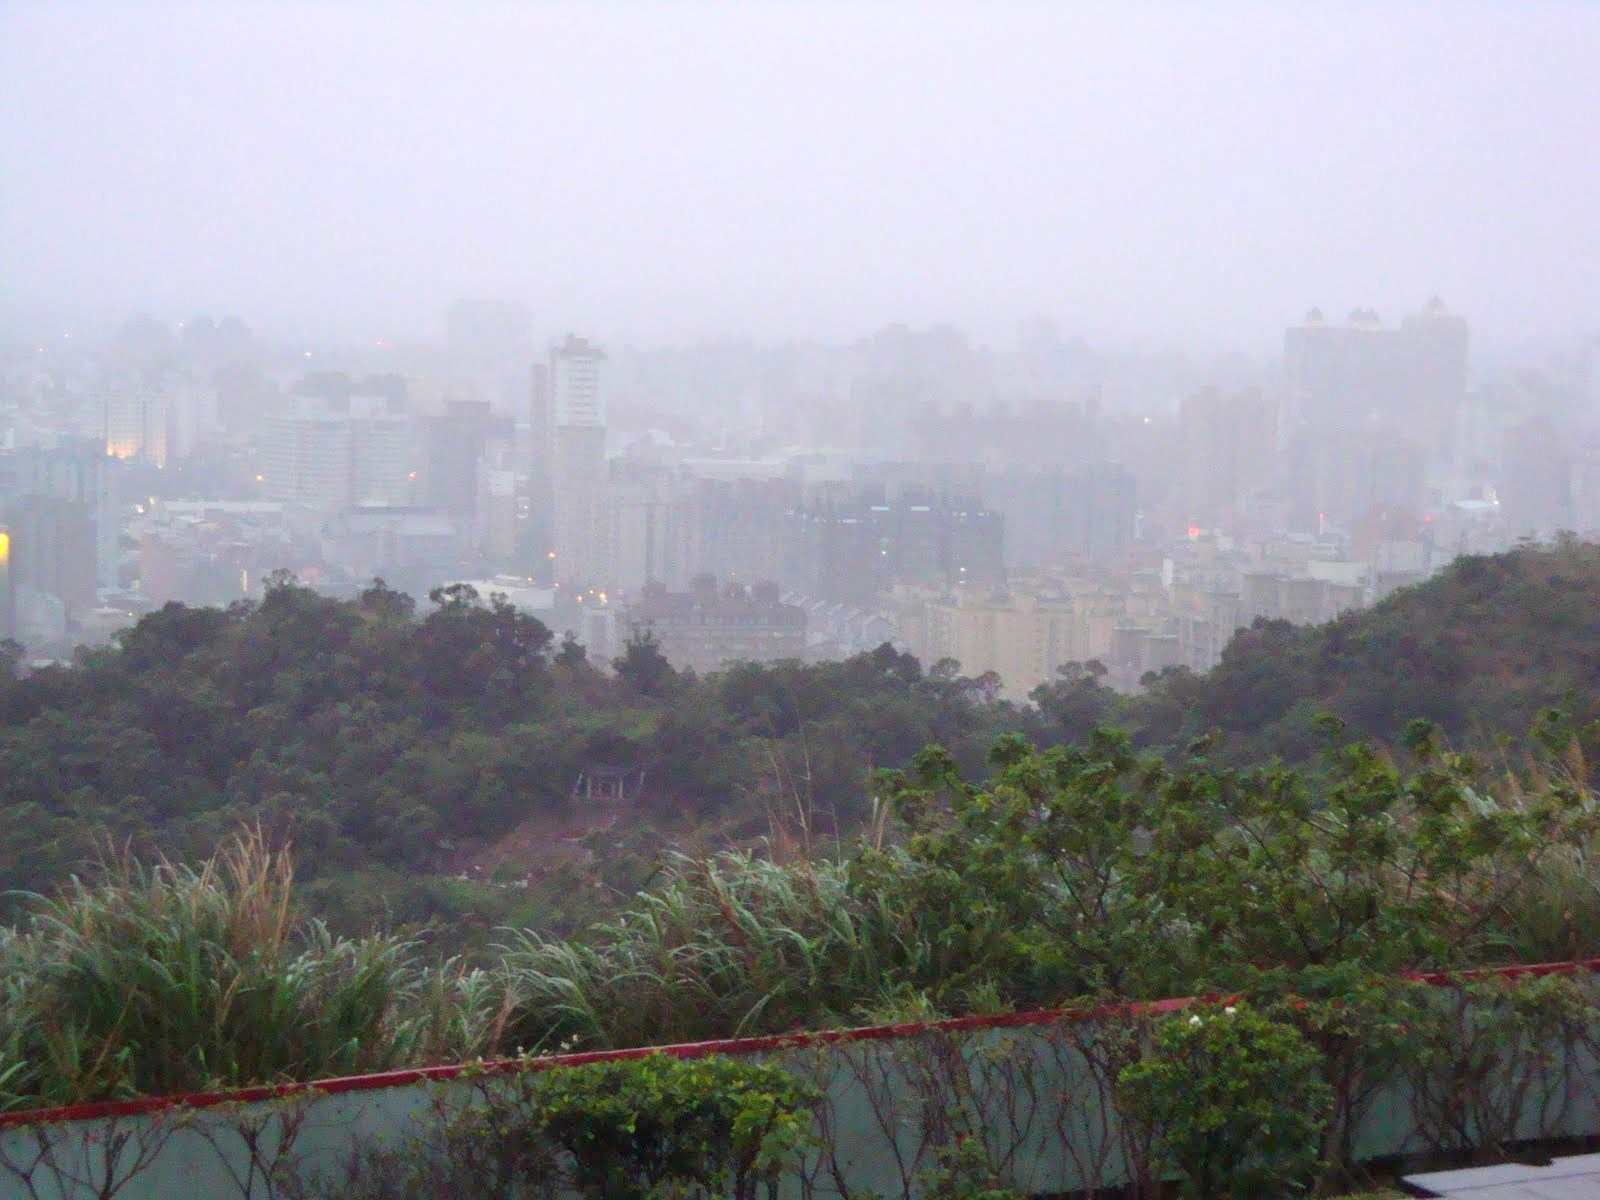
\includegraphics[height=2in]{notes/media/air_pollution.jpg}
  \end{center}
\end{frame}

\begin{frame}
  \frametitle{Набір даних}

  Загальний опис датасету:

  \begin{enumerate}
    \item Кількість рядків: 5\,882\,208
    \item Кількість стовпців: 25

    \begin{itemize}
      \item Числові: 19
      \item Факторні: 4
      \item Дата: 1
      \item Інші: 1
    \end{itemize}
  \end{enumerate}
\end{frame}

\begin{frame}
  \frametitle{Питання EDA}

  \begin{enumerate}
    \item Чи впливає швидкість вітру на концентрацію частинок PM2.5 і PM10?
    \item Чи існує кореляція між рівнем забруднення повітря і типом головного забруднювача
    в різних районах?
    \item Як зміни в концентрації озону  впливають на загальний рівень забруднення повітря?
    \item Які регіони мають найвищий середній рівень забруднення повітря протягом року?
    \item Як змінюється якість повітря протягом доби в різних районах?
  \end{enumerate}
\end{frame}

\begin{frame}
  \frametitle{Питання EDA}

  \begin{enumerate}
    \setcounter{enumi}{5}

    \item Як змінюється концентрація PM2.5 і PM10 в залежності від швидкості вітру і напрямку вітру
    в різних регіонах?
    \item Як змінився загальний рівень забруднення по регіонам після початку реформи?
    \item Чи існує залежність між початком реформ та показниками забруднення?
    \item Як змінюється якість повітря залежно від станції виміру у містах?
  \end{enumerate}
\end{frame}

\begin{frame}
  \section{Підготовка даних}

  \frametitle{Зміст}
  \tableofcontents[currentsection]
\end{frame}

\begin{frame}
  \frametitle{``Очищення'' даних}

  \begin{enumerate}
    \item Звели дати до одного формату.
    \item Замінили кодові значення (``$ \ $'', ``$-$'', ``ND'', -1, -999, 990) на NA.
    \item Перетворили текстові колонки на категорійні.
    \item Видалили стовпці, які не знадобляться для аналізу.
    \item Видалили стовпці, у яких більше $50\%$ пропущених даних.
    \item Додали стовпець \textit{after\_reform}, що визначає, чи вимір
    якості повітря був здійснений після реформи (\textit{17 грудня 2017 року})
  \end{enumerate}
\end{frame}

\begin{frame}
  \frametitle{``Очищення'' даних}

  Був отриманий набір даних, що складається з таких змінних:

  \begin{itemize}
    \item Числові - 11
    \item Факторні - 3
    \item Дата - 1
    \item Логічні - 1
  \end{itemize}
\end{frame}

\begin{frame}
  \frametitle{Зменшення датасету}

  \begin{enumerate}
    \item Для пришвидшення обчислень та побудови графіків в певних випадках будемо використовувати
    окремий набір даних, в якому виміри починаються з 2023 року.
    \item Таким чином цей набір даних має 1\,232\,994 рядків.
    \item Надалі будемо зазначати на якому наборі даних був виконаний аналіз. Зменшений
    датасет назвемо \textit{trimmed}, а весь очищений набір даних -- \textit{tidy}.
  \end{enumerate}

\end{frame}

\begin{frame}
  \section{Характеристика даних}

  \frametitle{Зміст}
  \tableofcontents[currentsection]
\end{frame}

\begin{frame}
  \frametitle{Пропущені дані}

  Був використаний \textit{tidy} набір даних.

  \begin{center}
    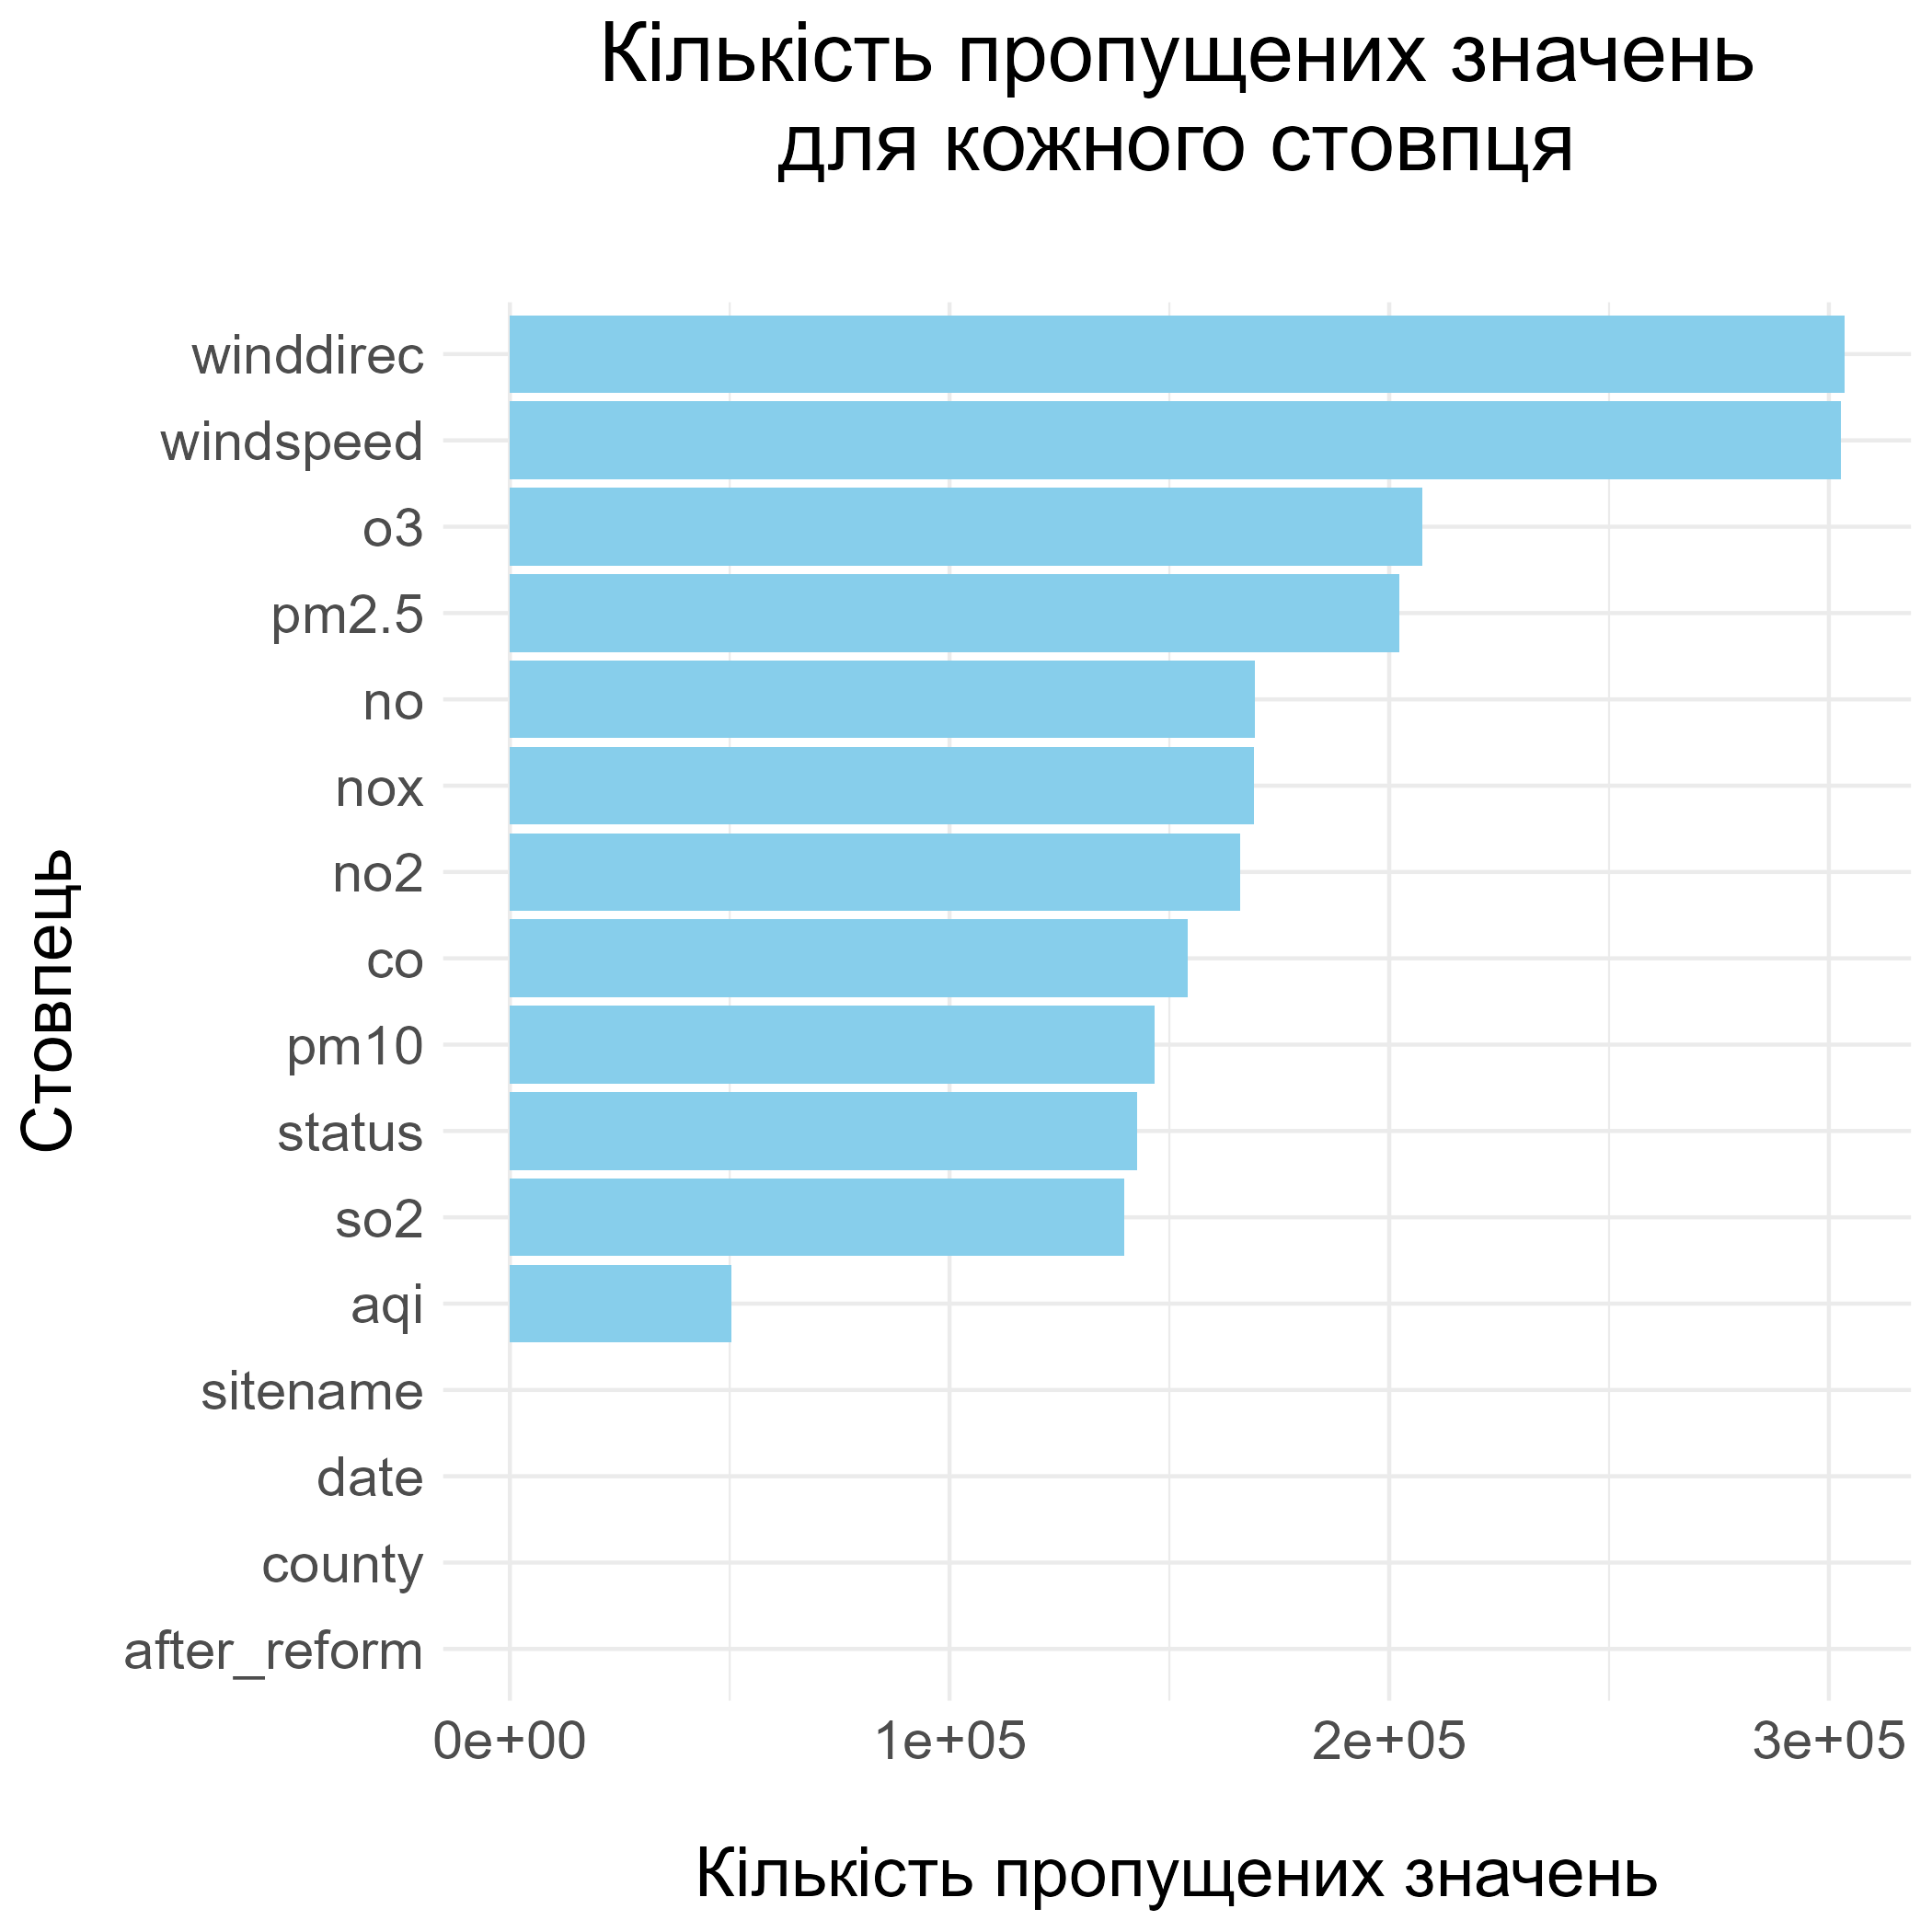
\includegraphics[height=2.8in]{plots/missed_data.png}
  \end{center}
\end{frame}

\begin{frame}
  \frametitle{Викиди}

  Був використаний \textit{trimmed} набір даних.

  Для пошуку викидів використаємо \textit{фільтр Гампеля}:

  \begin{center}
    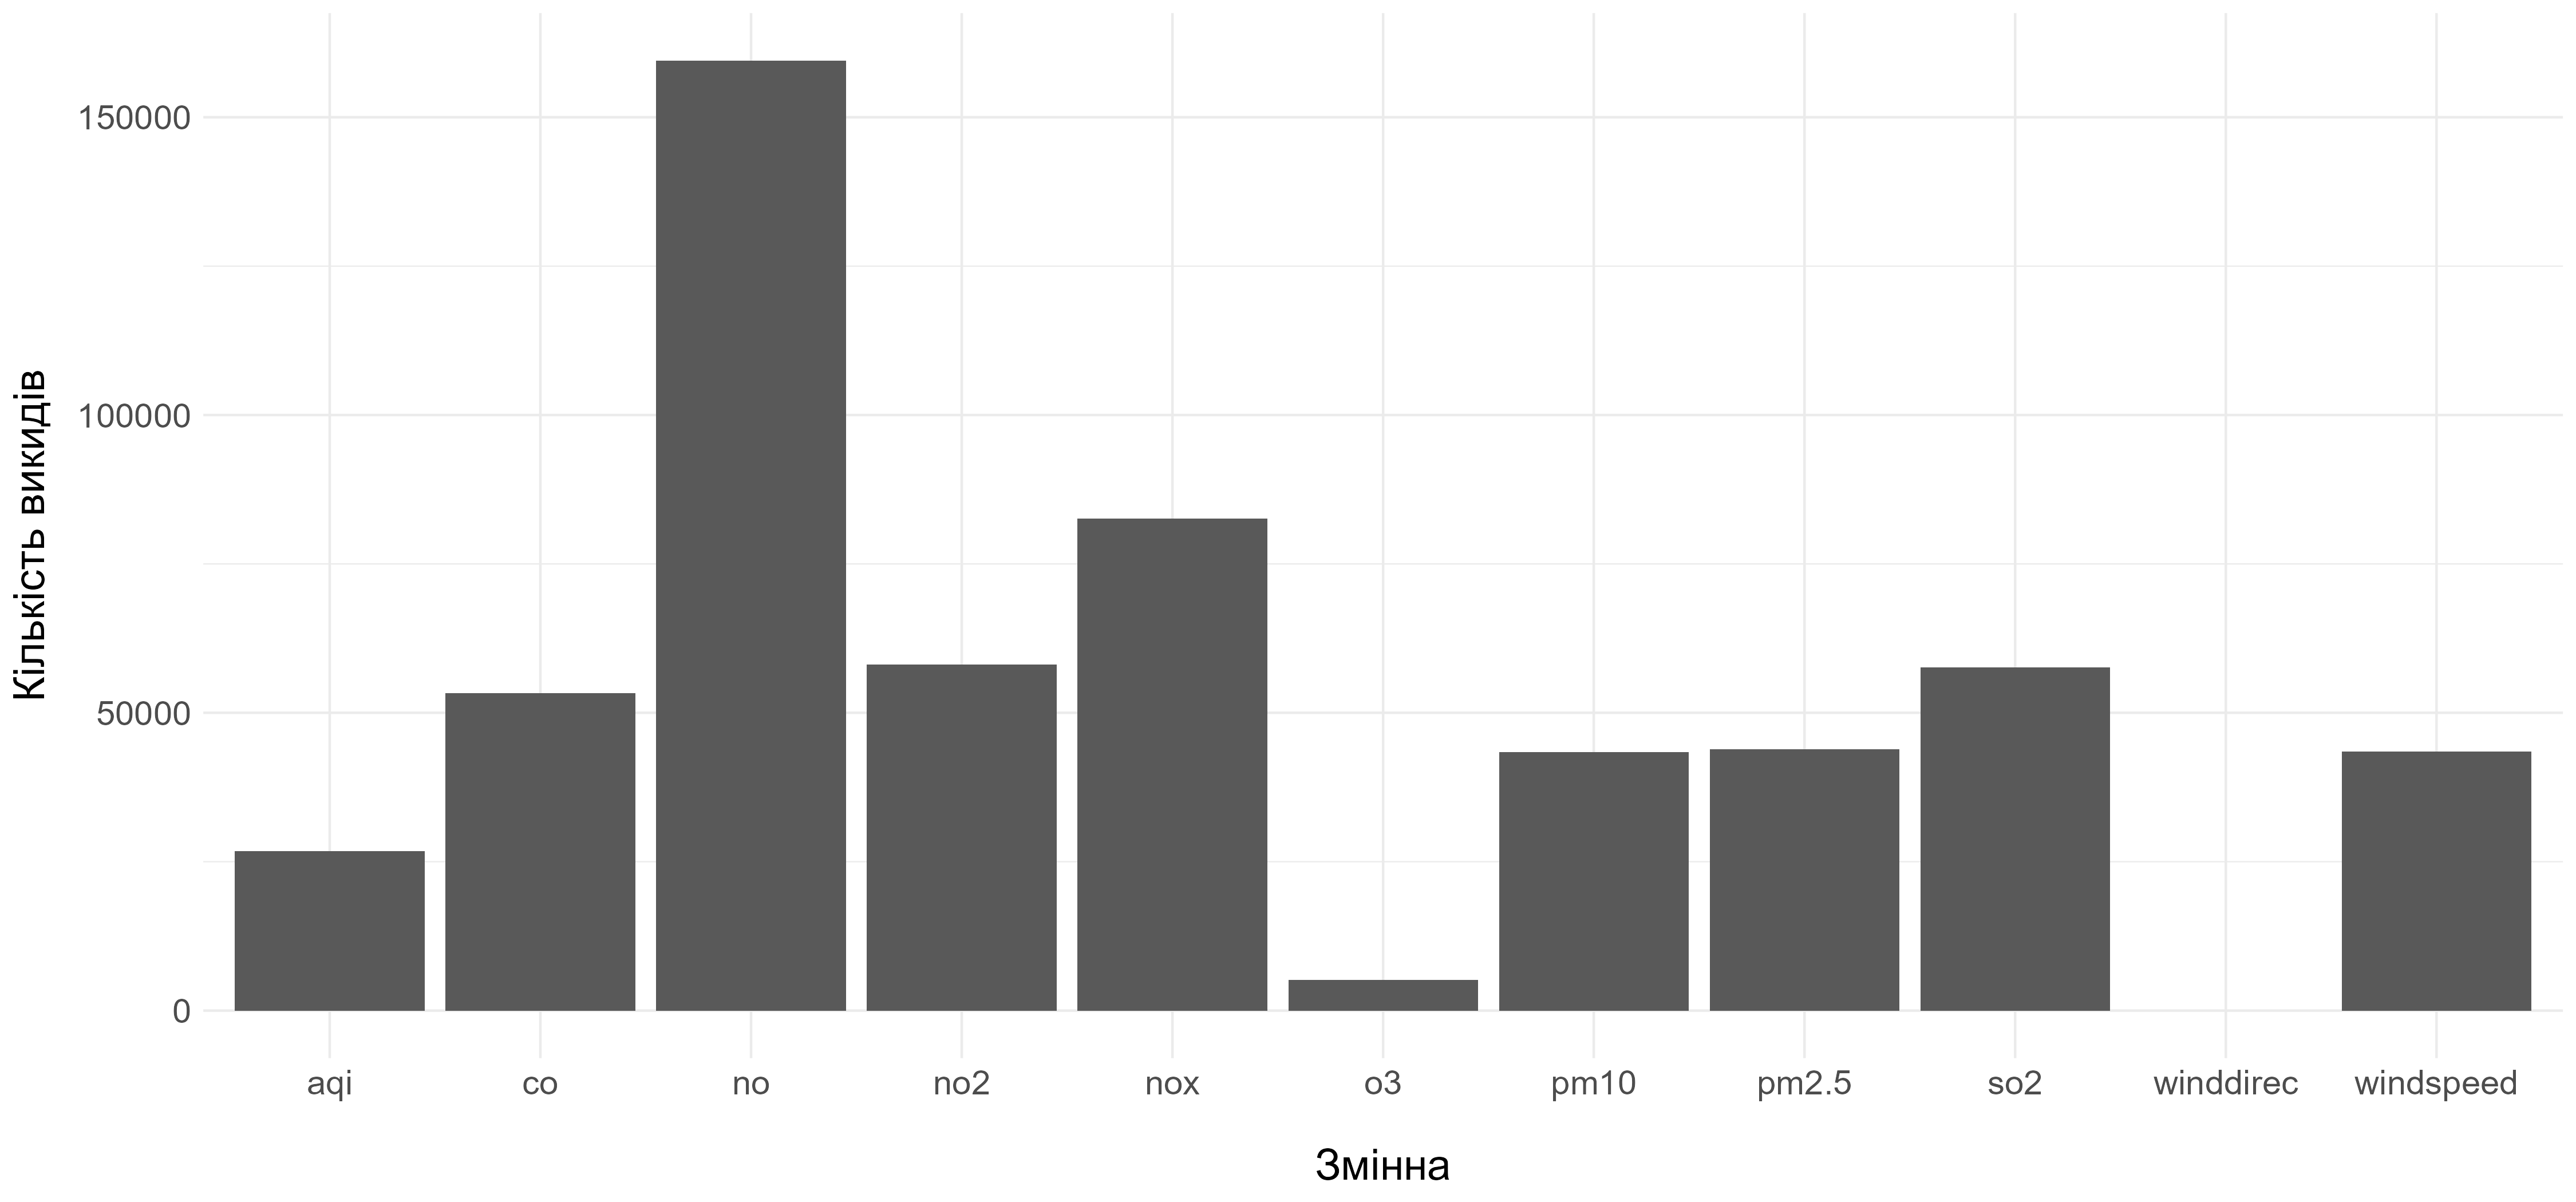
\includegraphics[height=2.5in]{plots/outliers/count-bar.png}
  \end{center}
\end{frame}

\begin{frame}
  \frametitle{Викиди}

  \begin{center}
    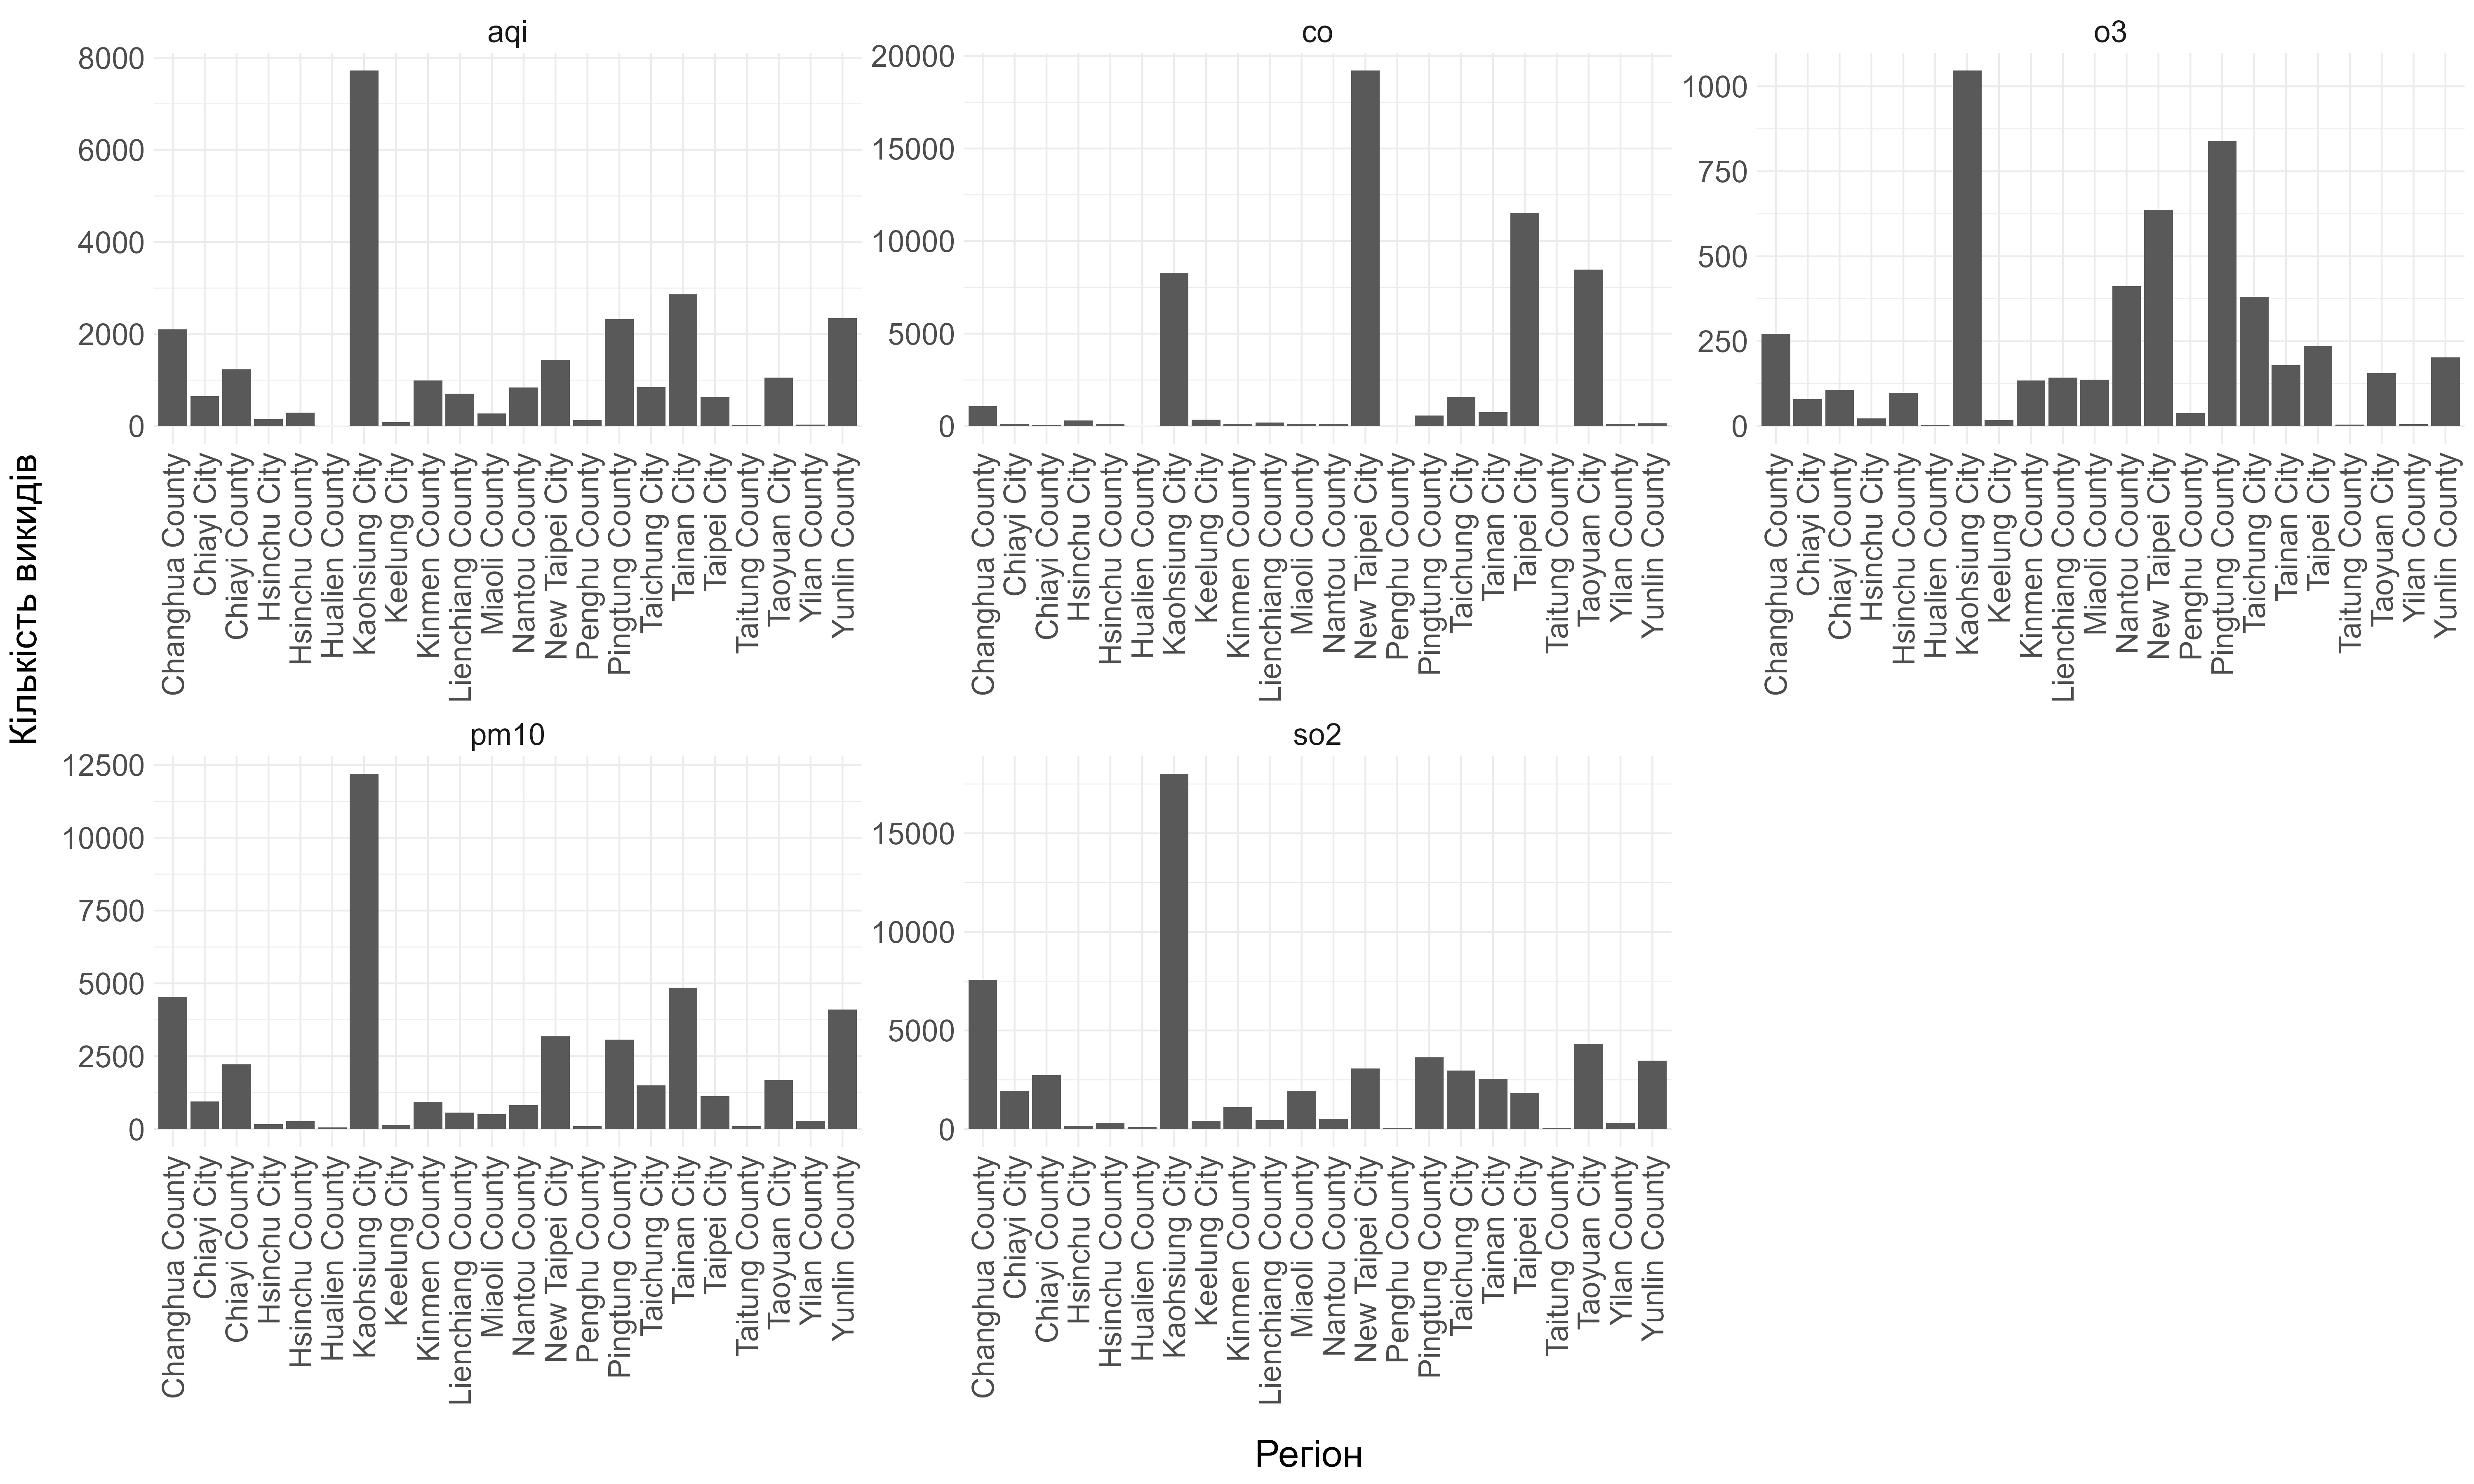
\includegraphics[height=3in]{plots/outliers/count-bar-county-p1.png}
  \end{center}
\end{frame}

\begin{frame}
  \frametitle{Викиди}

  \begin{center}
    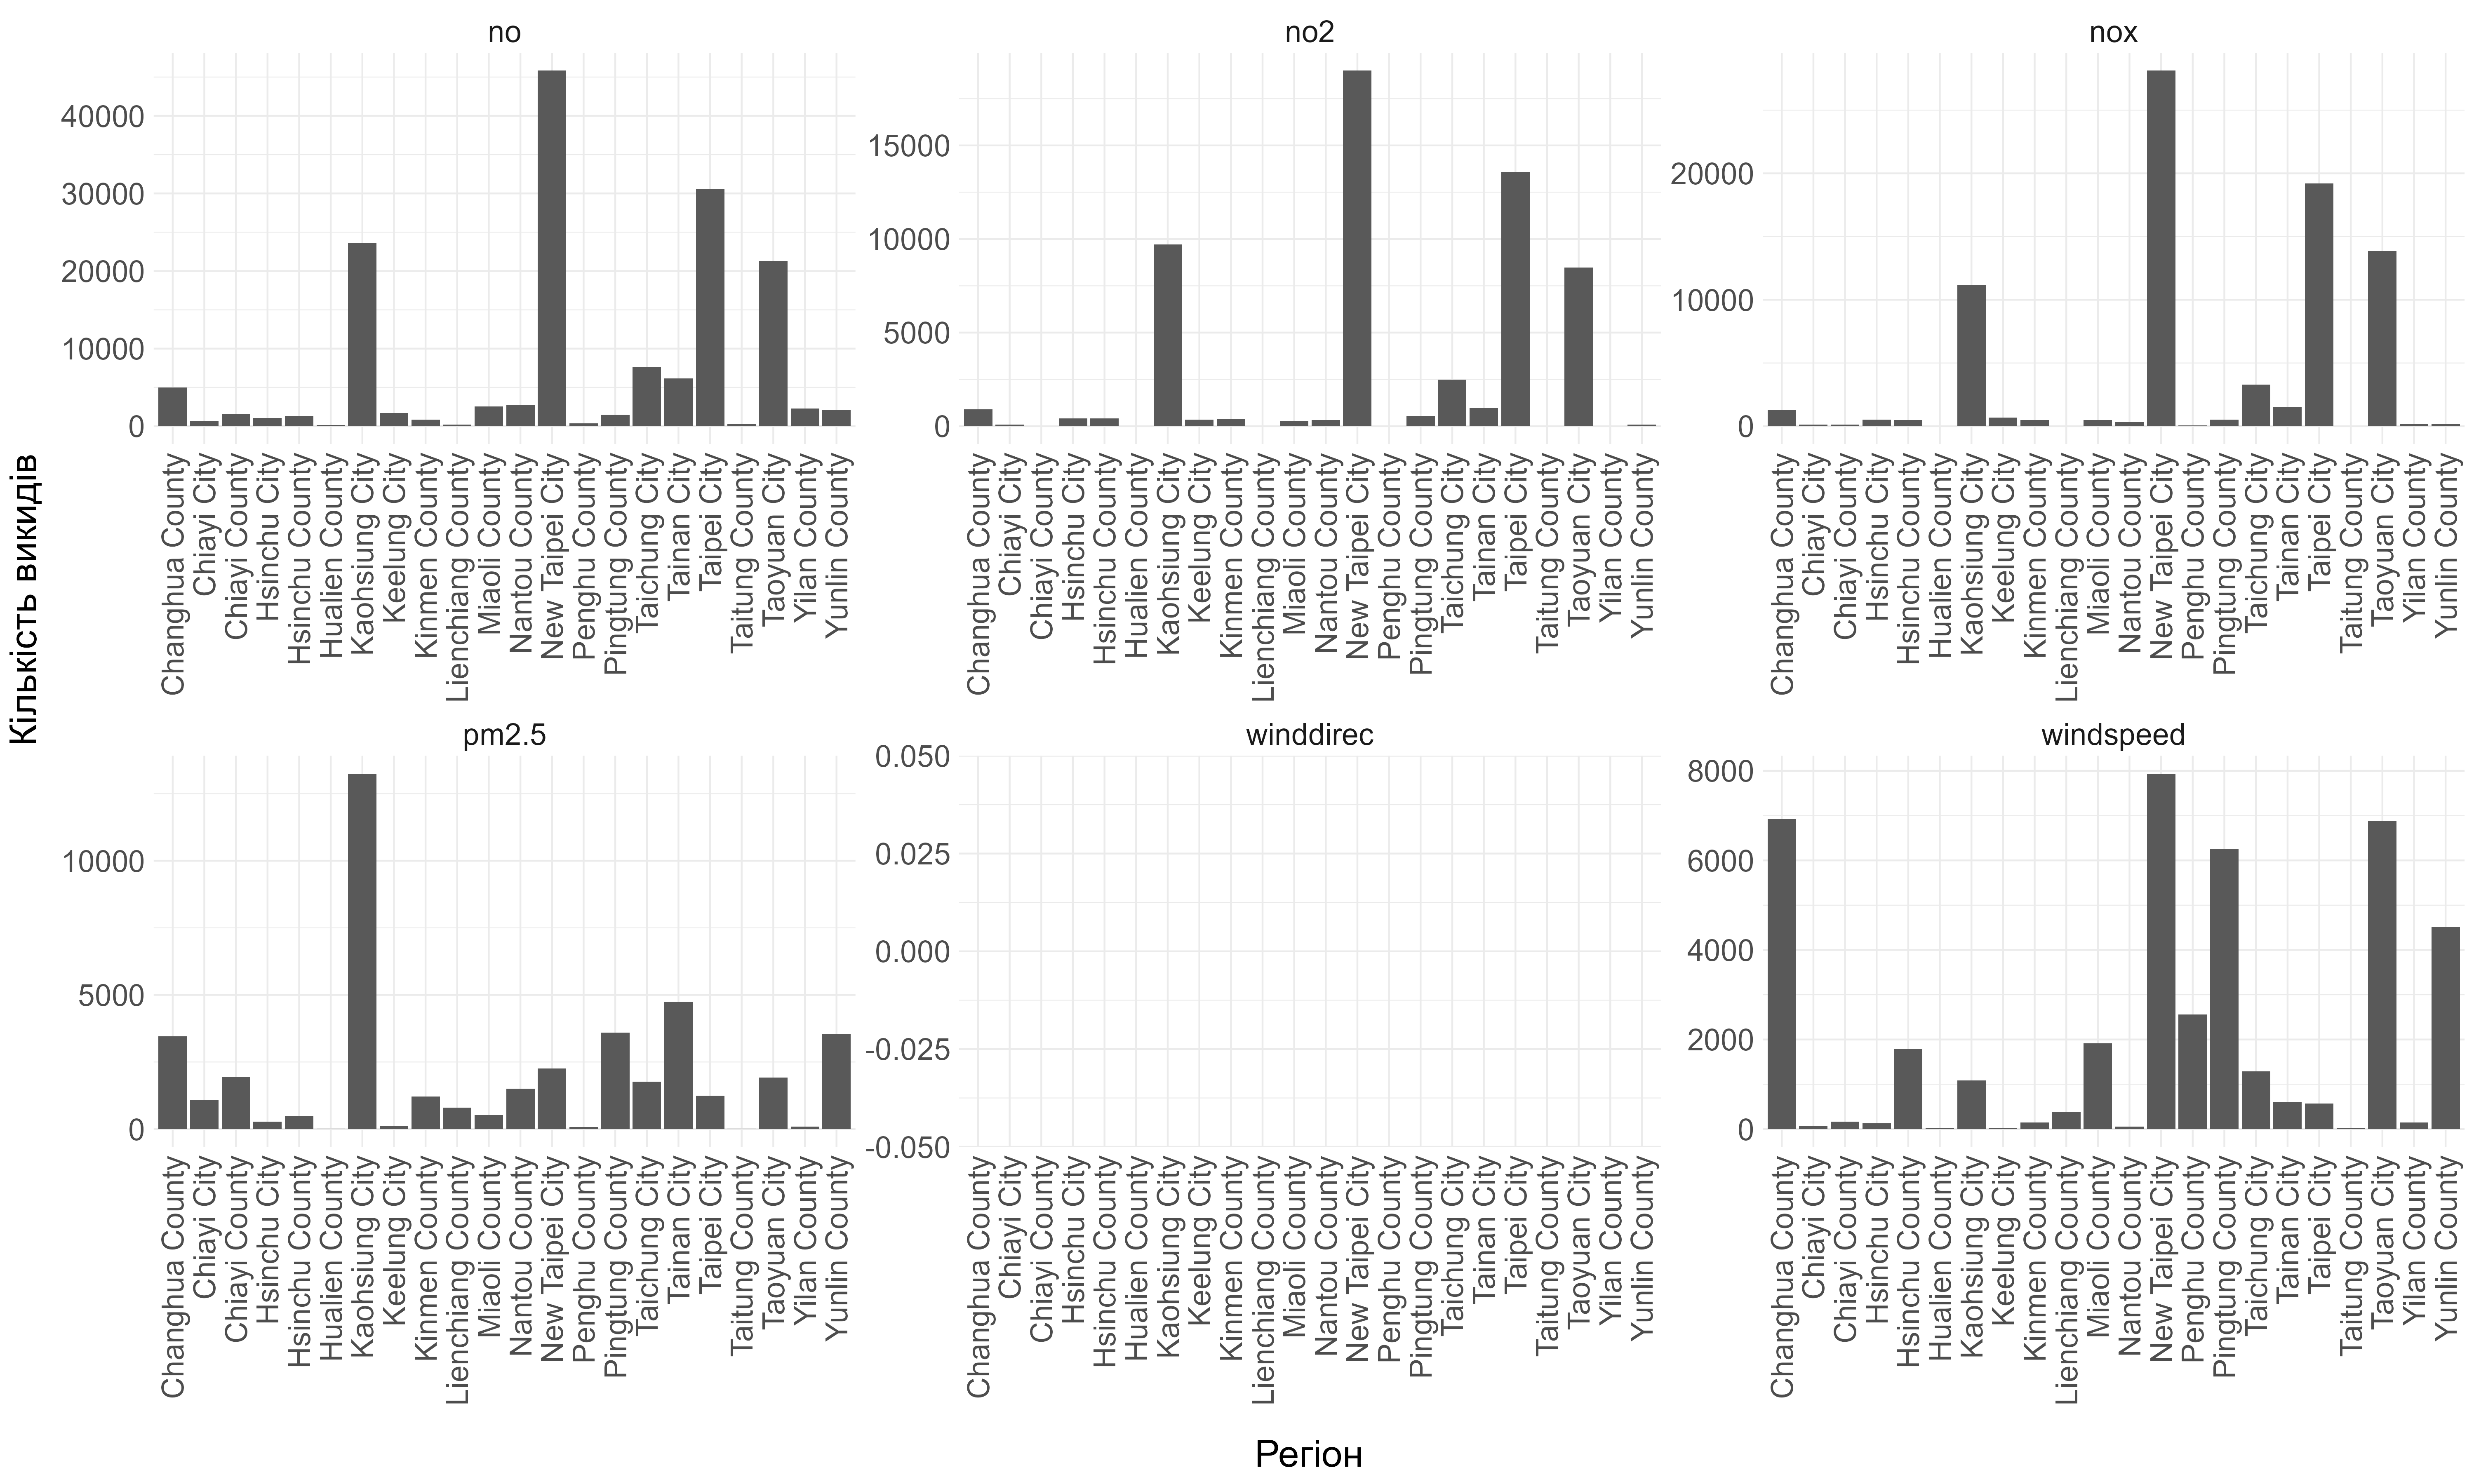
\includegraphics[height=3in]{plots/outliers/count-bar-county-p2.png}
  \end{center}
\end{frame}

\begin{frame}
  \frametitle{Викиди}

  \begin{center}
    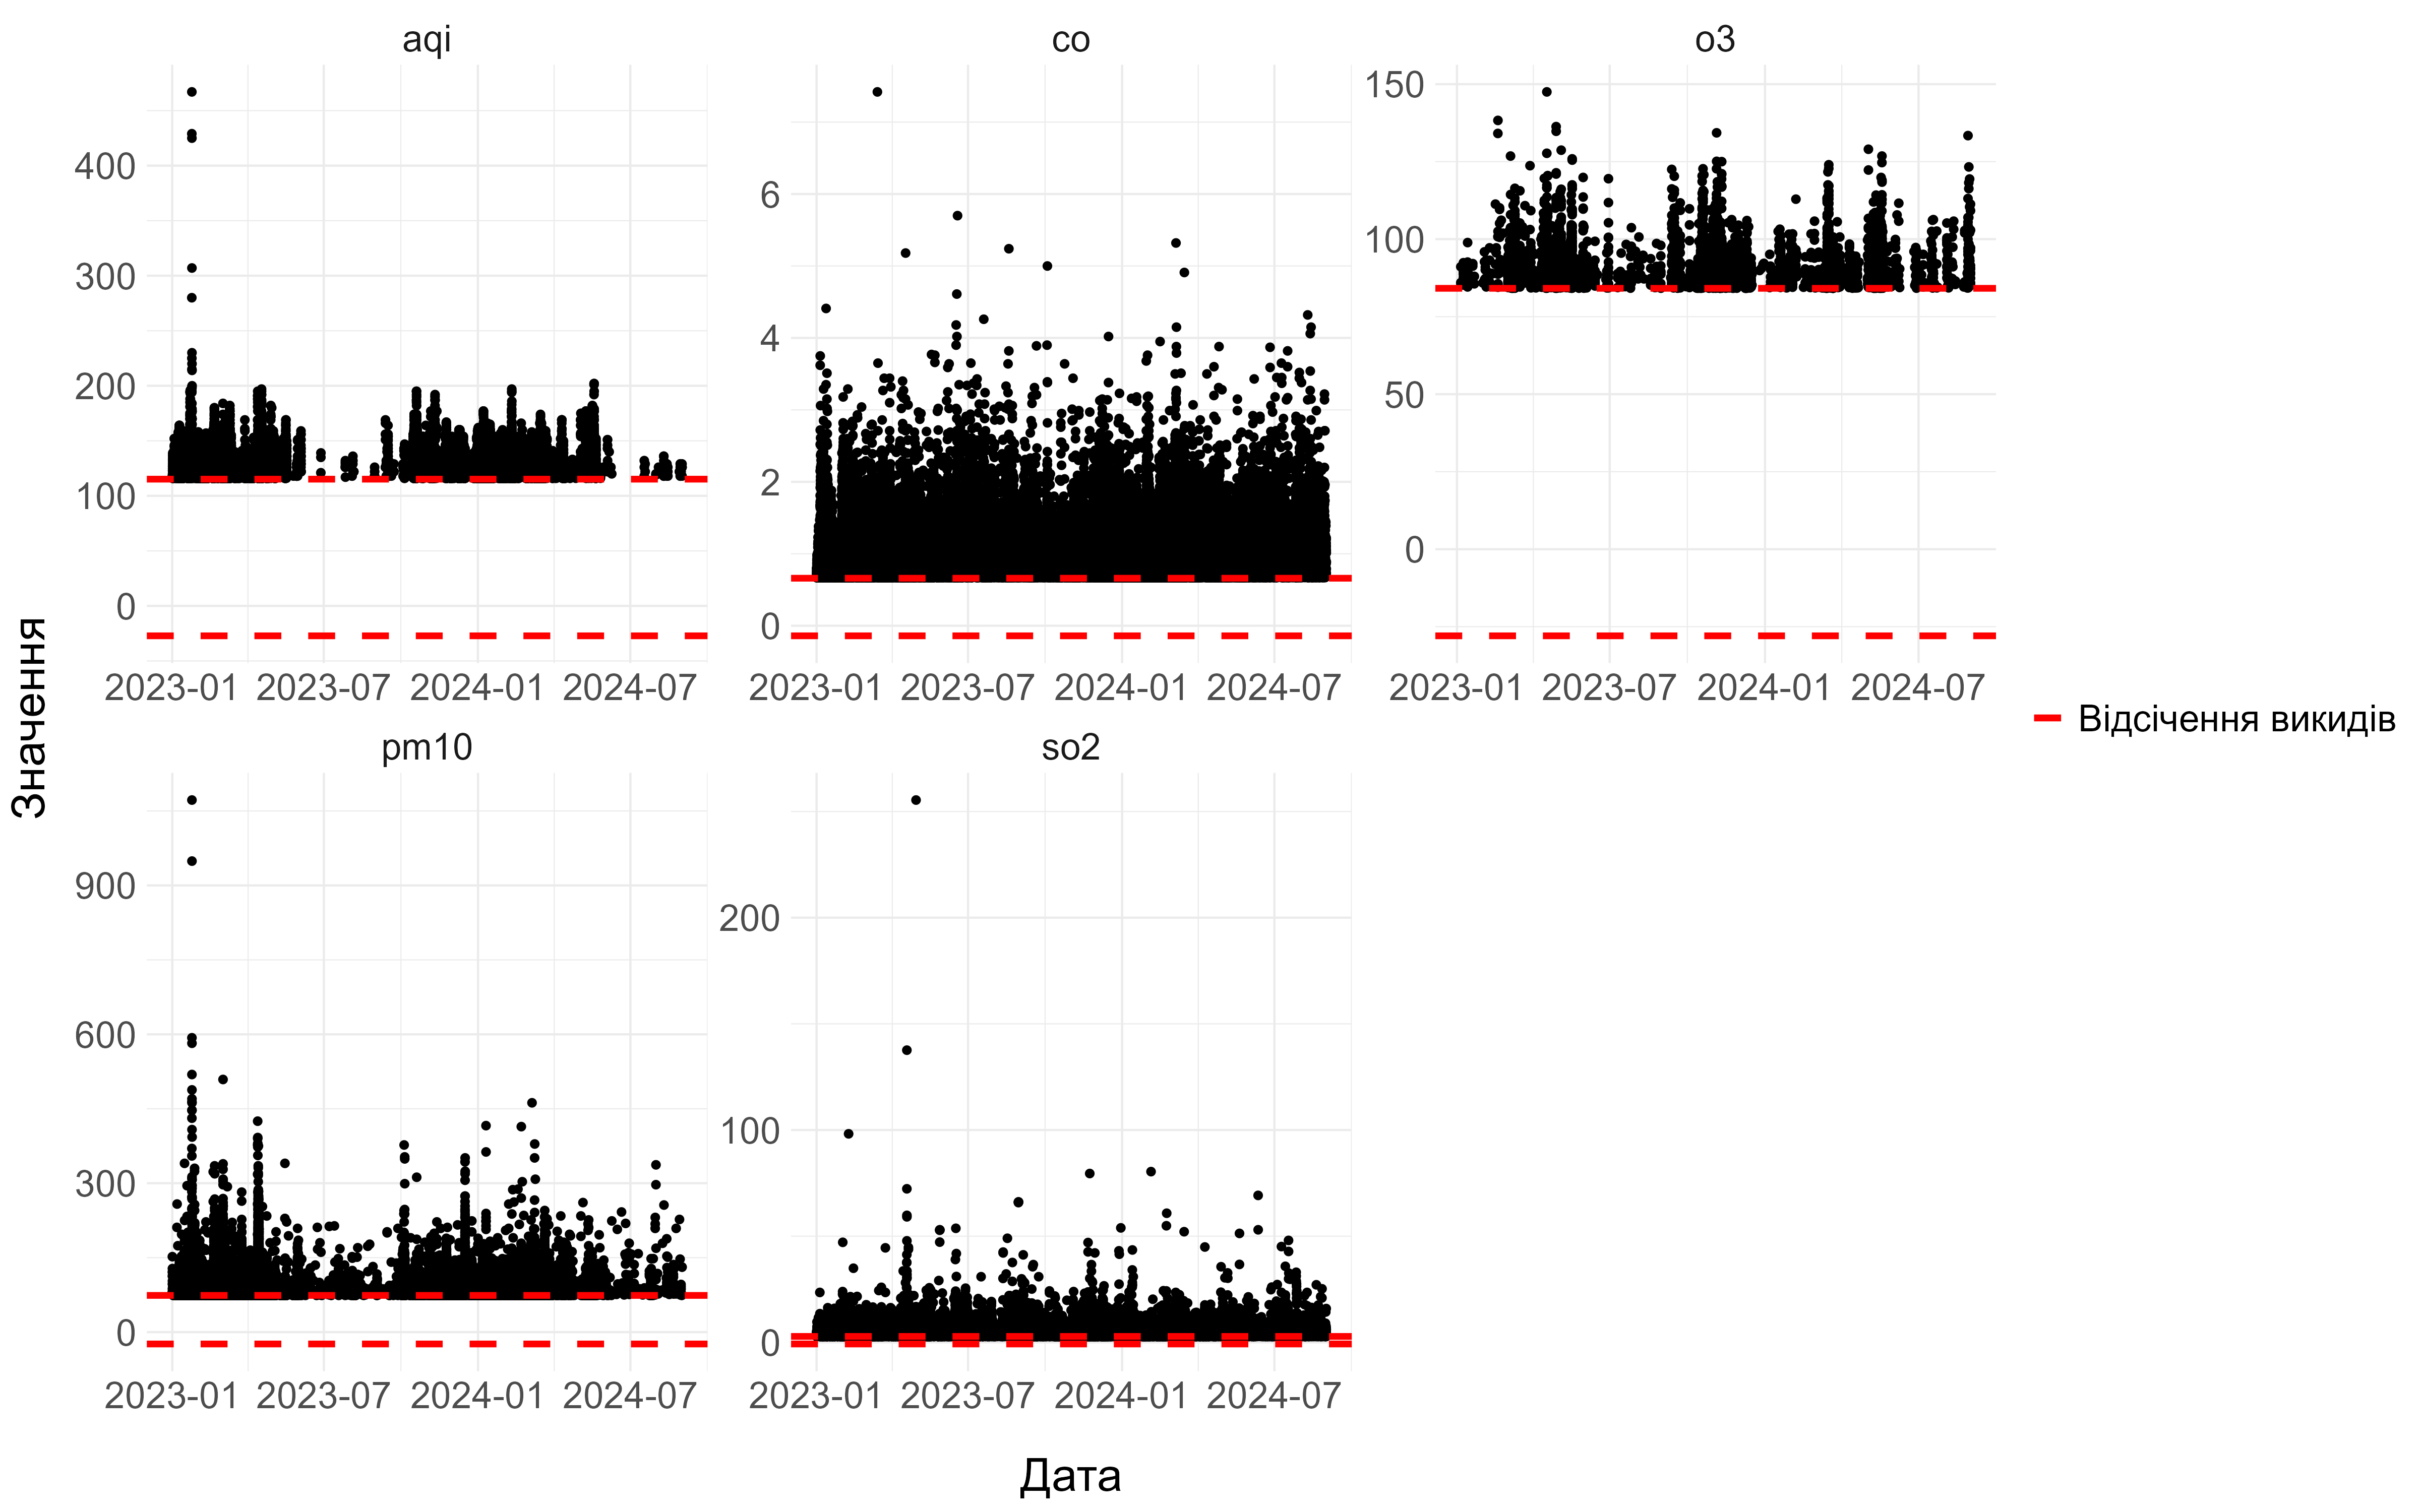
\includegraphics[height=3in]{plots/outliers/scatter-p1.png}
  \end{center}
\end{frame}

\begin{frame}
  \frametitle{Викиди}

  \begin{center}
    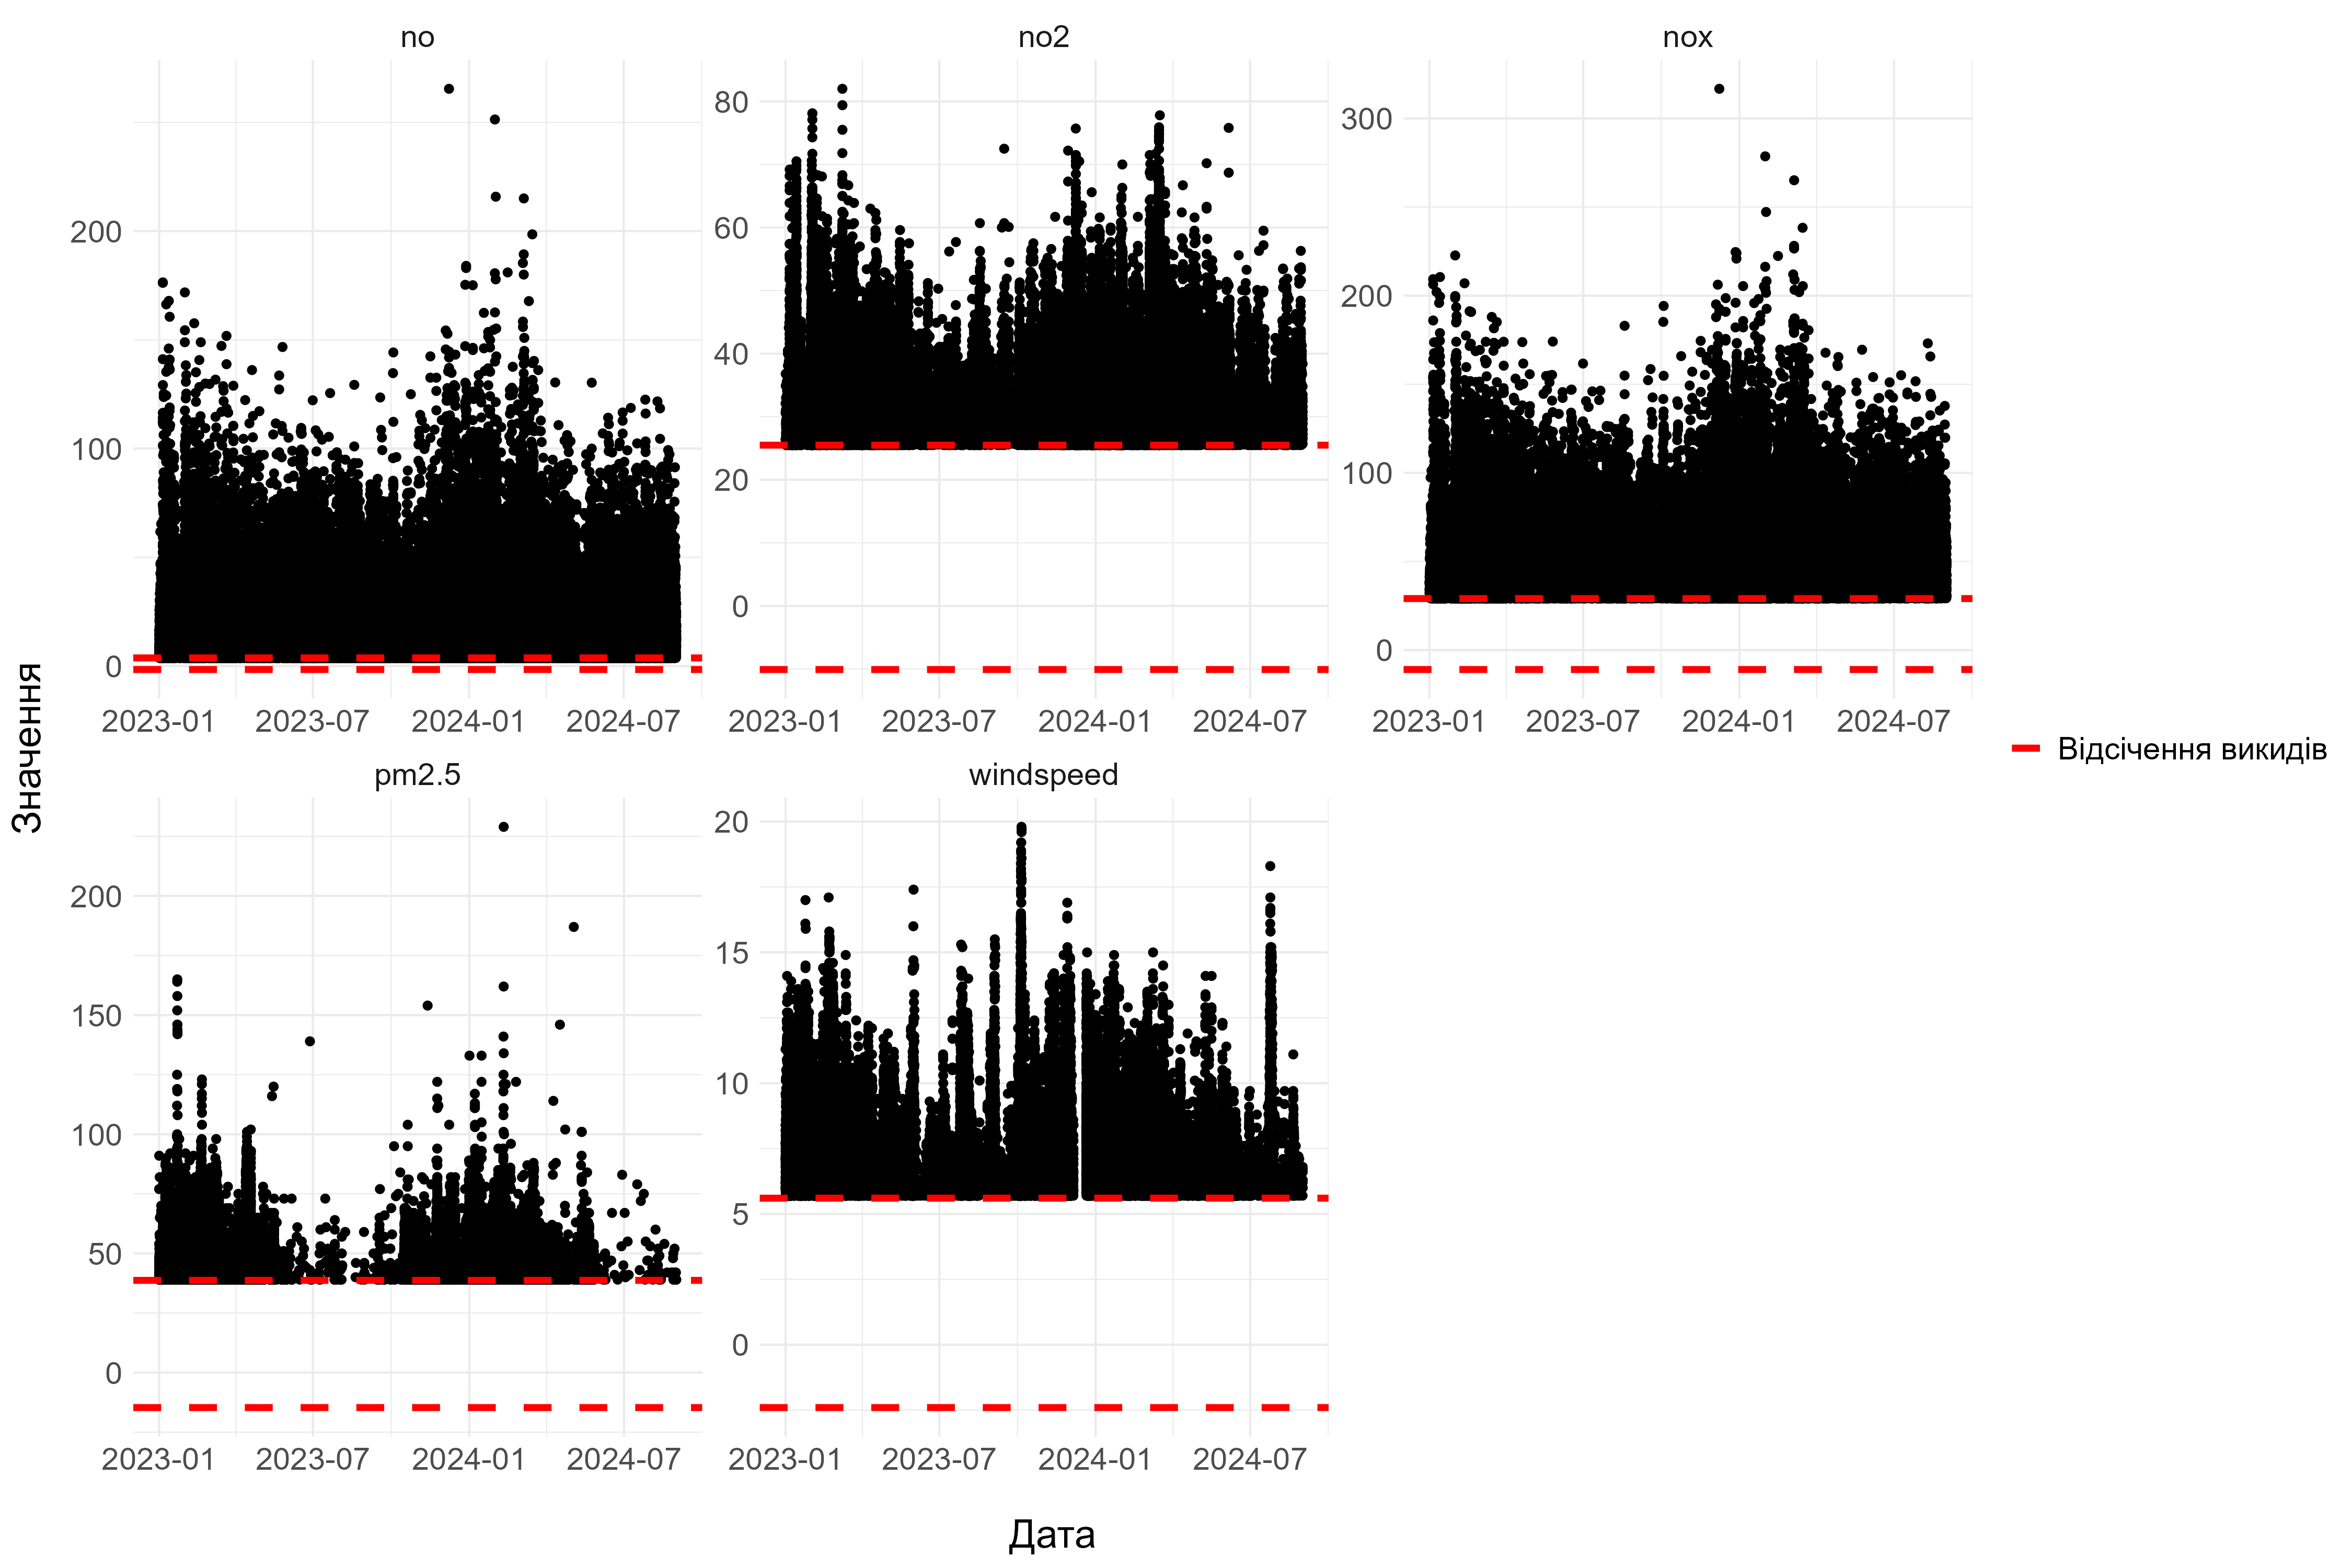
\includegraphics[height=3in]{plots/outliers/scatter-p2.png}
  \end{center}
\end{frame}

\begin{frame}
  \frametitle{Викиди}

  \begin{enumerate}
    \item На діаграмі розсіювання можна помітити значення, які набагато більші за
    інші викиди. Можна припустити, що вони є помилками датників, які вимірювали якість
    повітря.
    \item Було прийнято рішення не змінювати значення, або видаляти викиди.
    Натомість будемо використовувати міри, які більш стійкі до викидів.
  \end{enumerate}
\end{frame}

\begin{frame}
  \frametitle{Розподіли змінних}

  Для побудови QQ-графіків, випадковим чином виберемо з датасету 10\,000 рядків.

  \begin{center}
    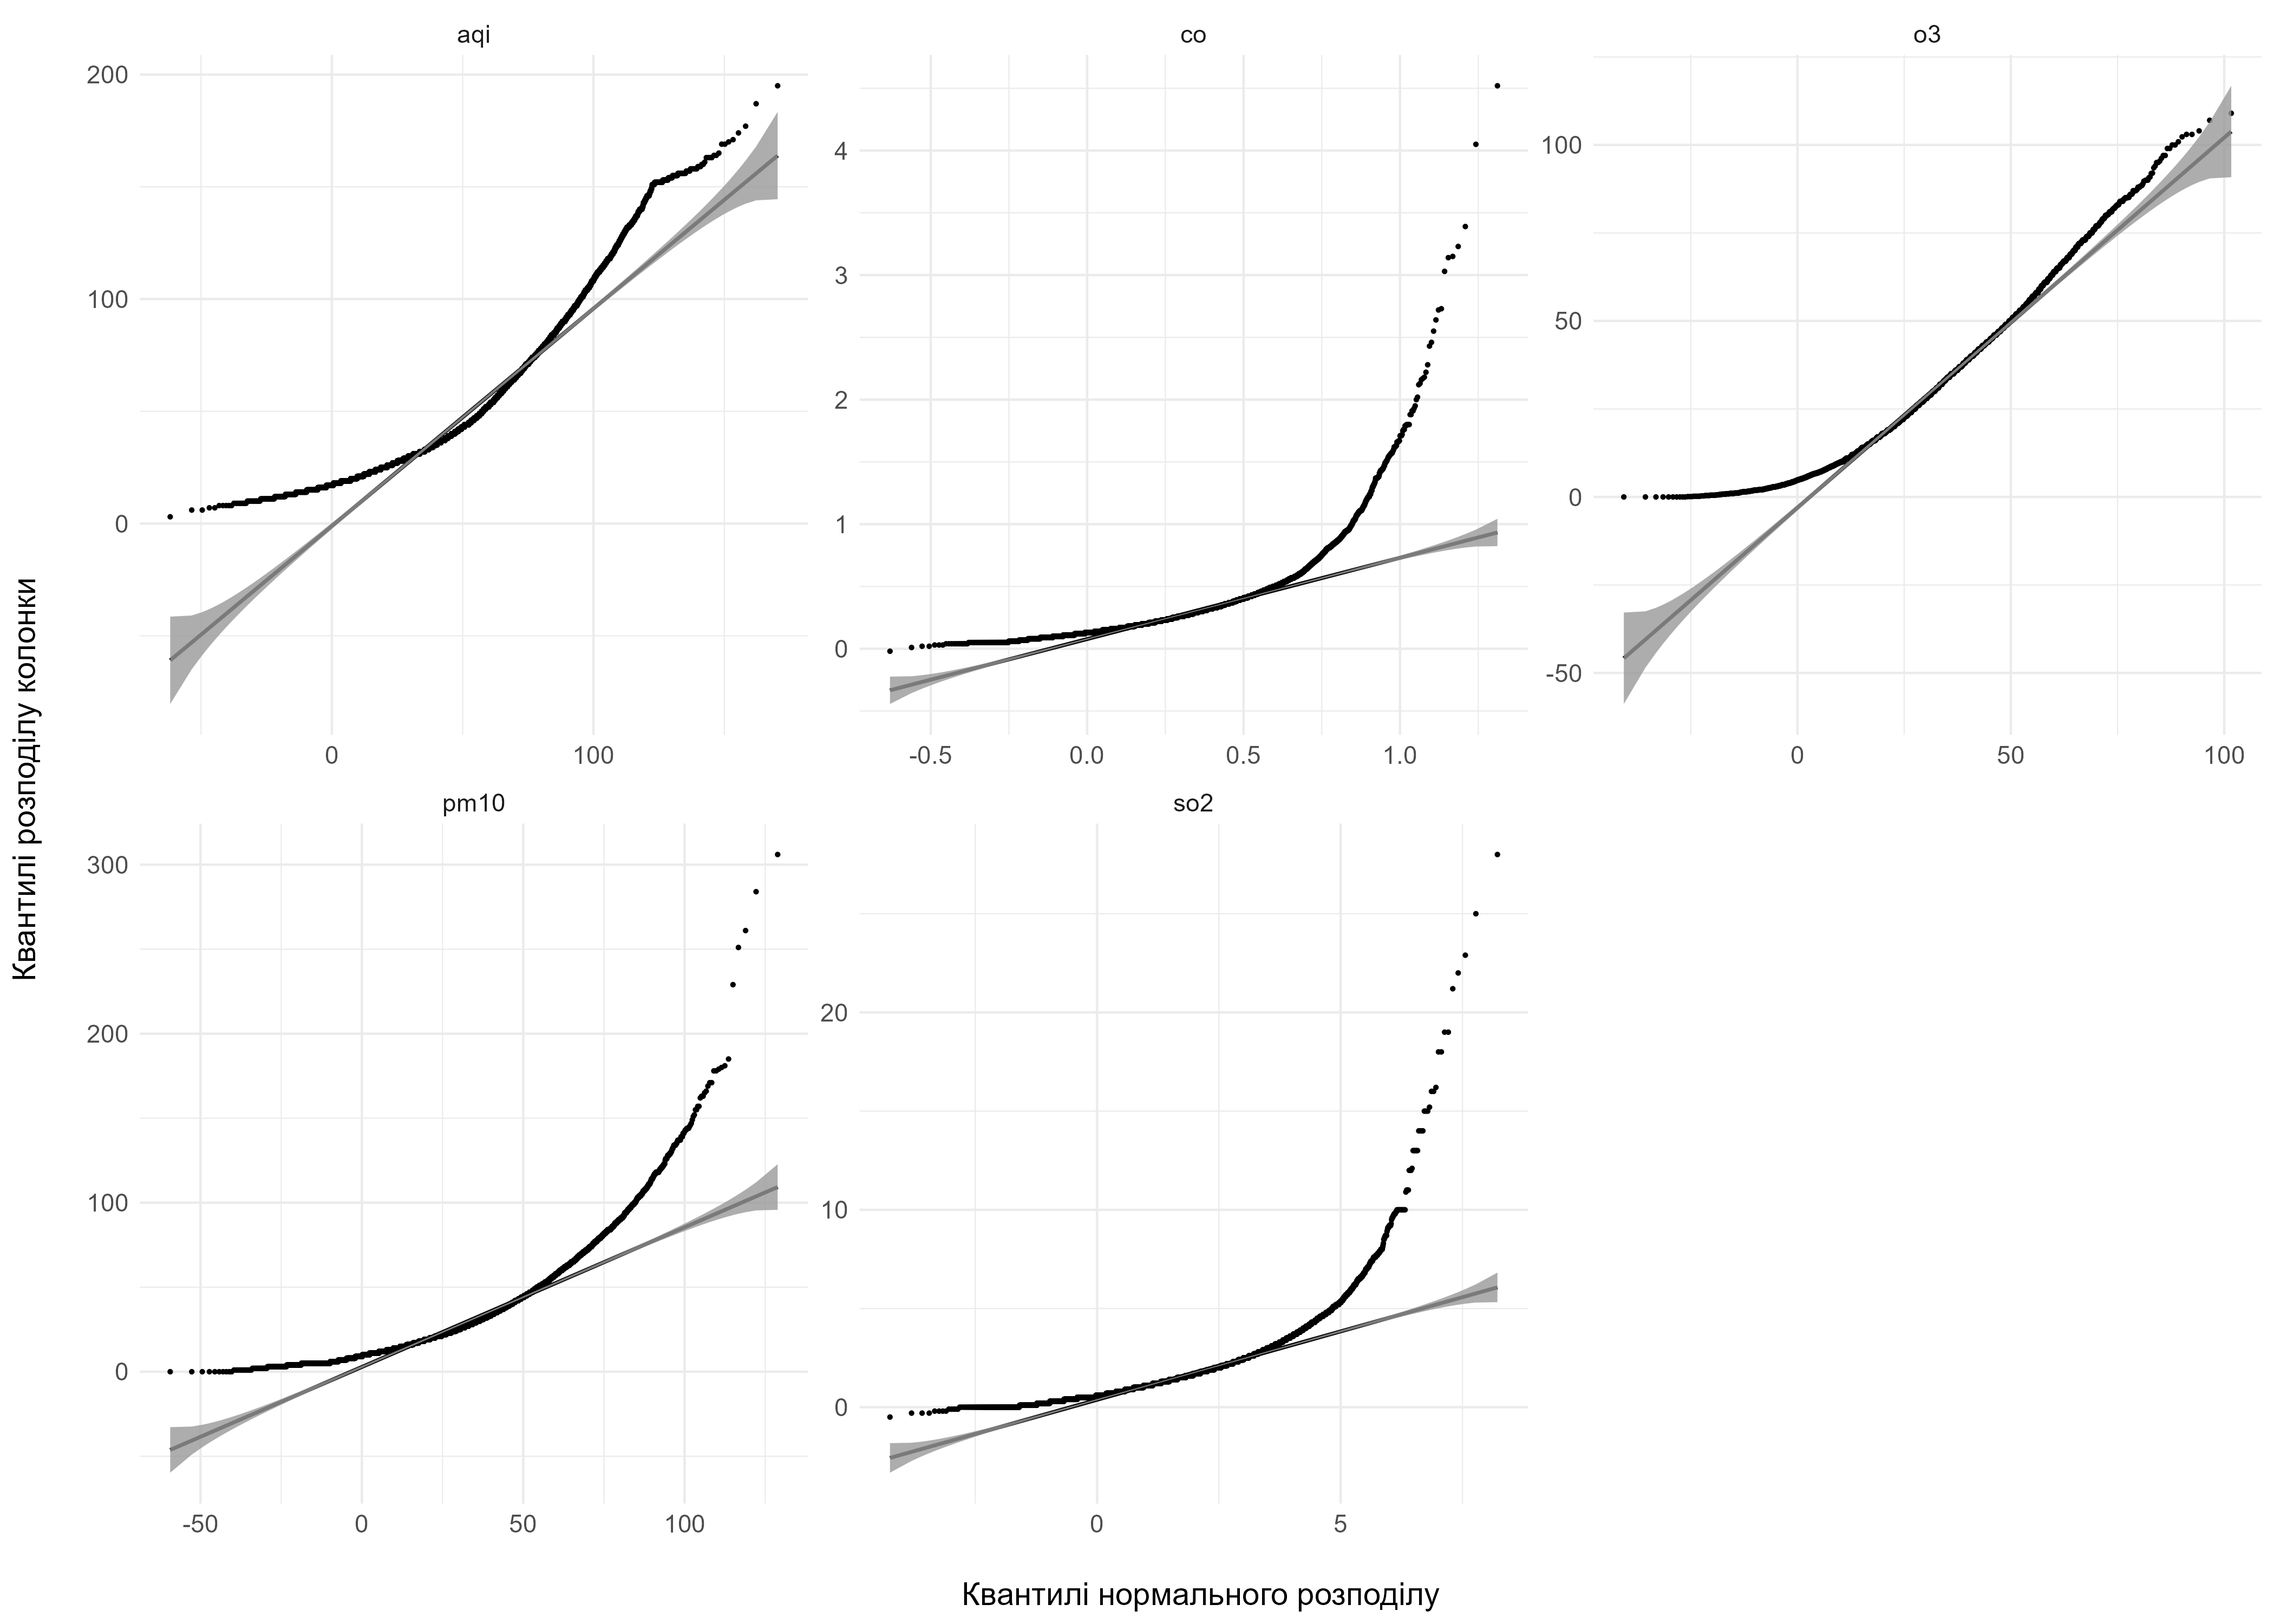
\includegraphics[height=2.5in]{plots/qq_tidy/qq-p1.png}
  \end{center}
\end{frame}

\begin{frame}
  \frametitle{Розподіли змінних}

  \begin{center}
    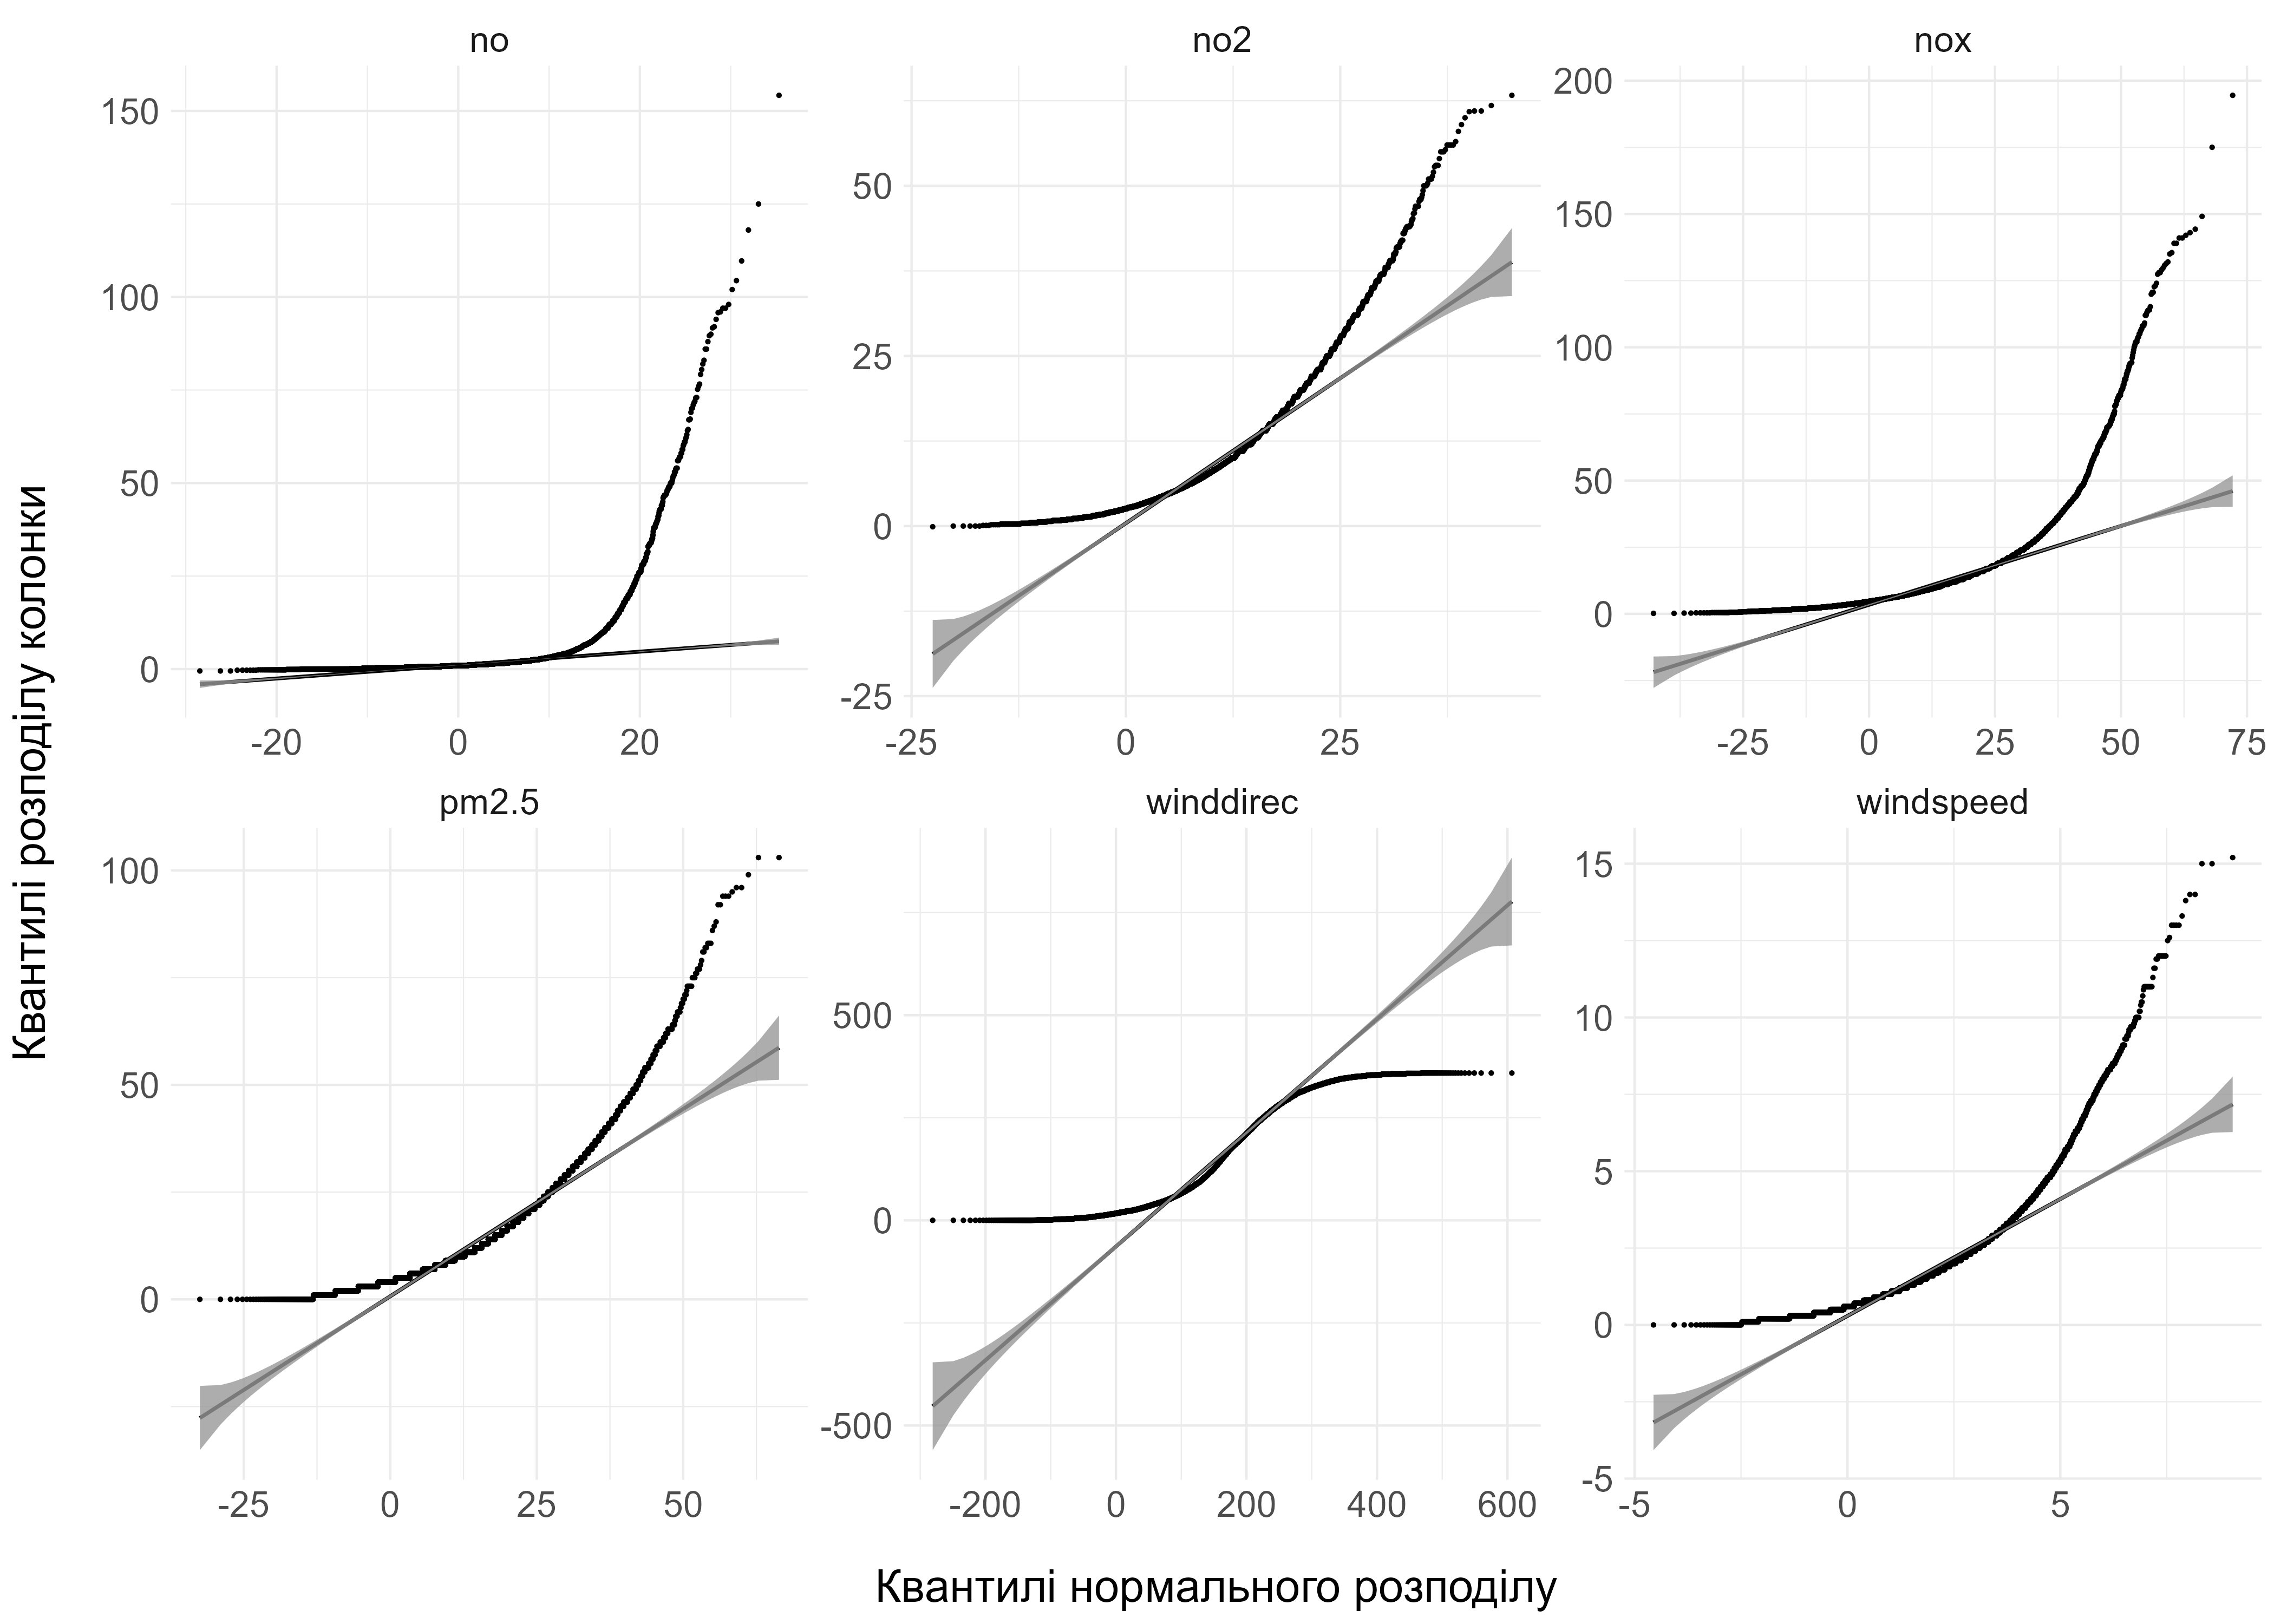
\includegraphics[height=3in]{plots/qq_tidy/qq-p2.png}
  \end{center}
\end{frame}

\begin{frame}
  \frametitle{Розподіли змінних}

  Розподіл змінних (крім \textit{winddirect} і \textit{o3}) ближче до логнормального, ніж нормального:

  \begin{center}
    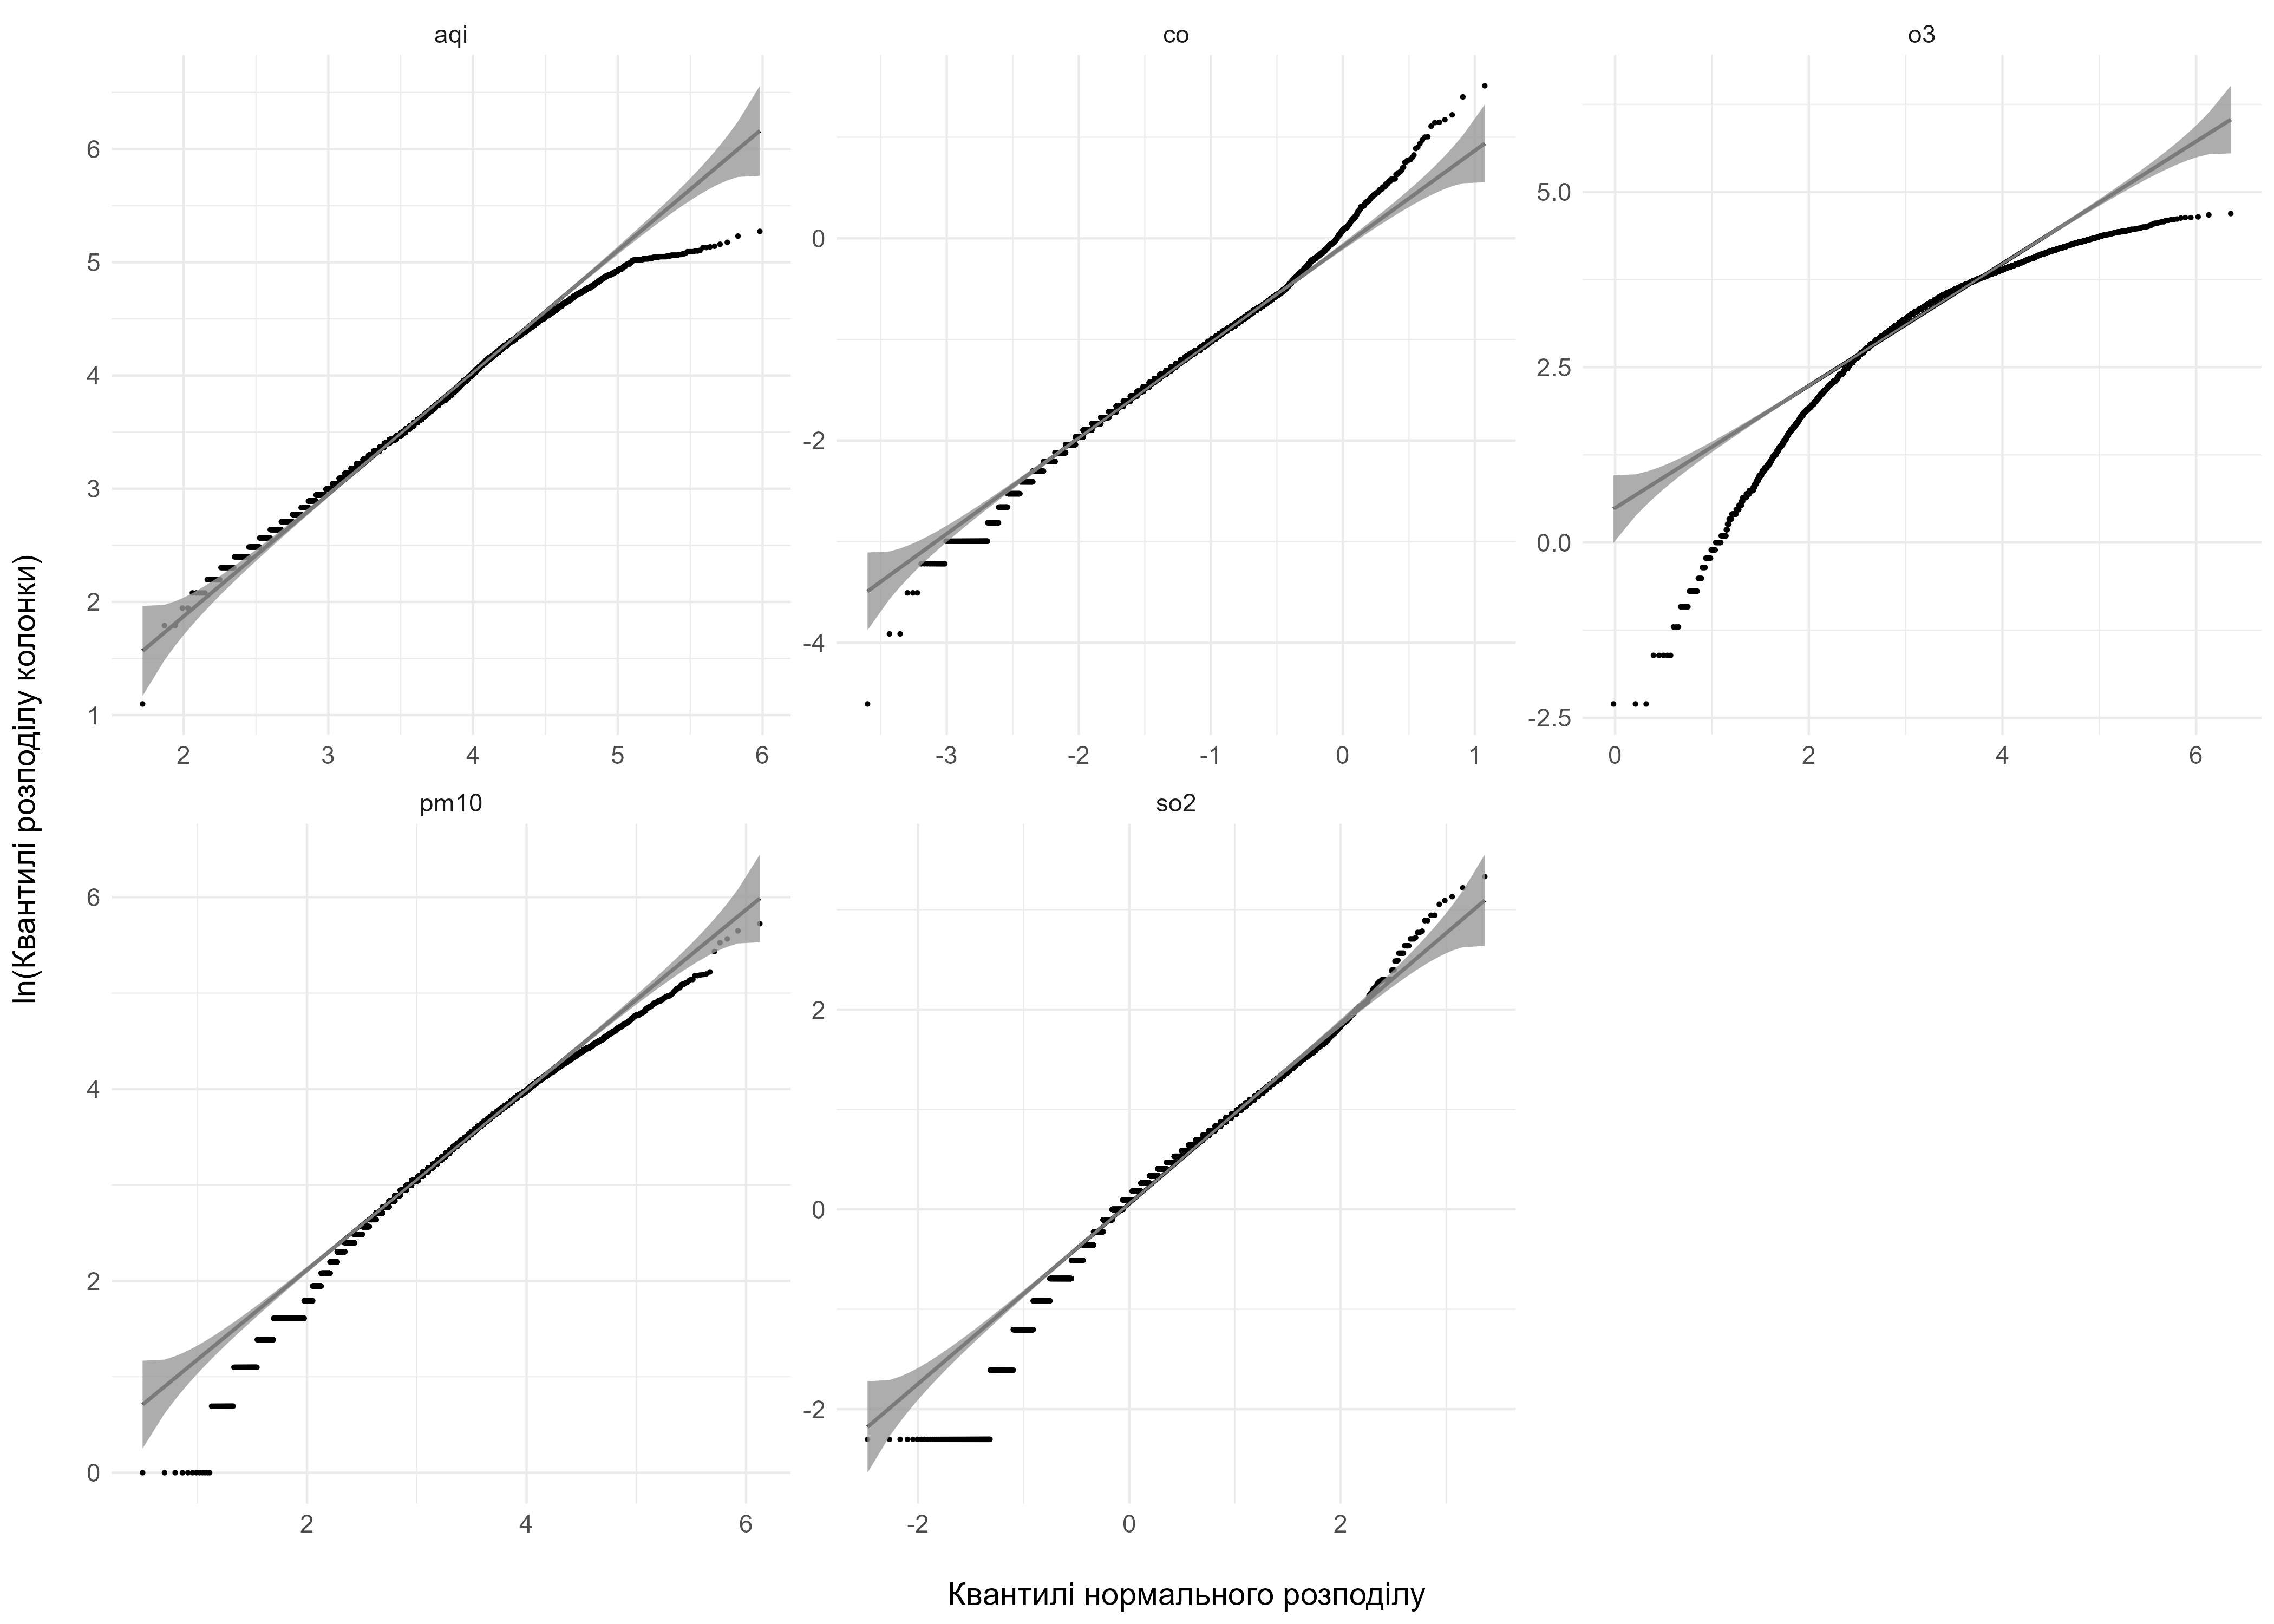
\includegraphics[height=2.5in]{plots/qq_tidy/qq-log-p1.png}
  \end{center}
\end{frame}

\begin{frame}
  \frametitle{Розподіли змінних}

  \begin{center}
    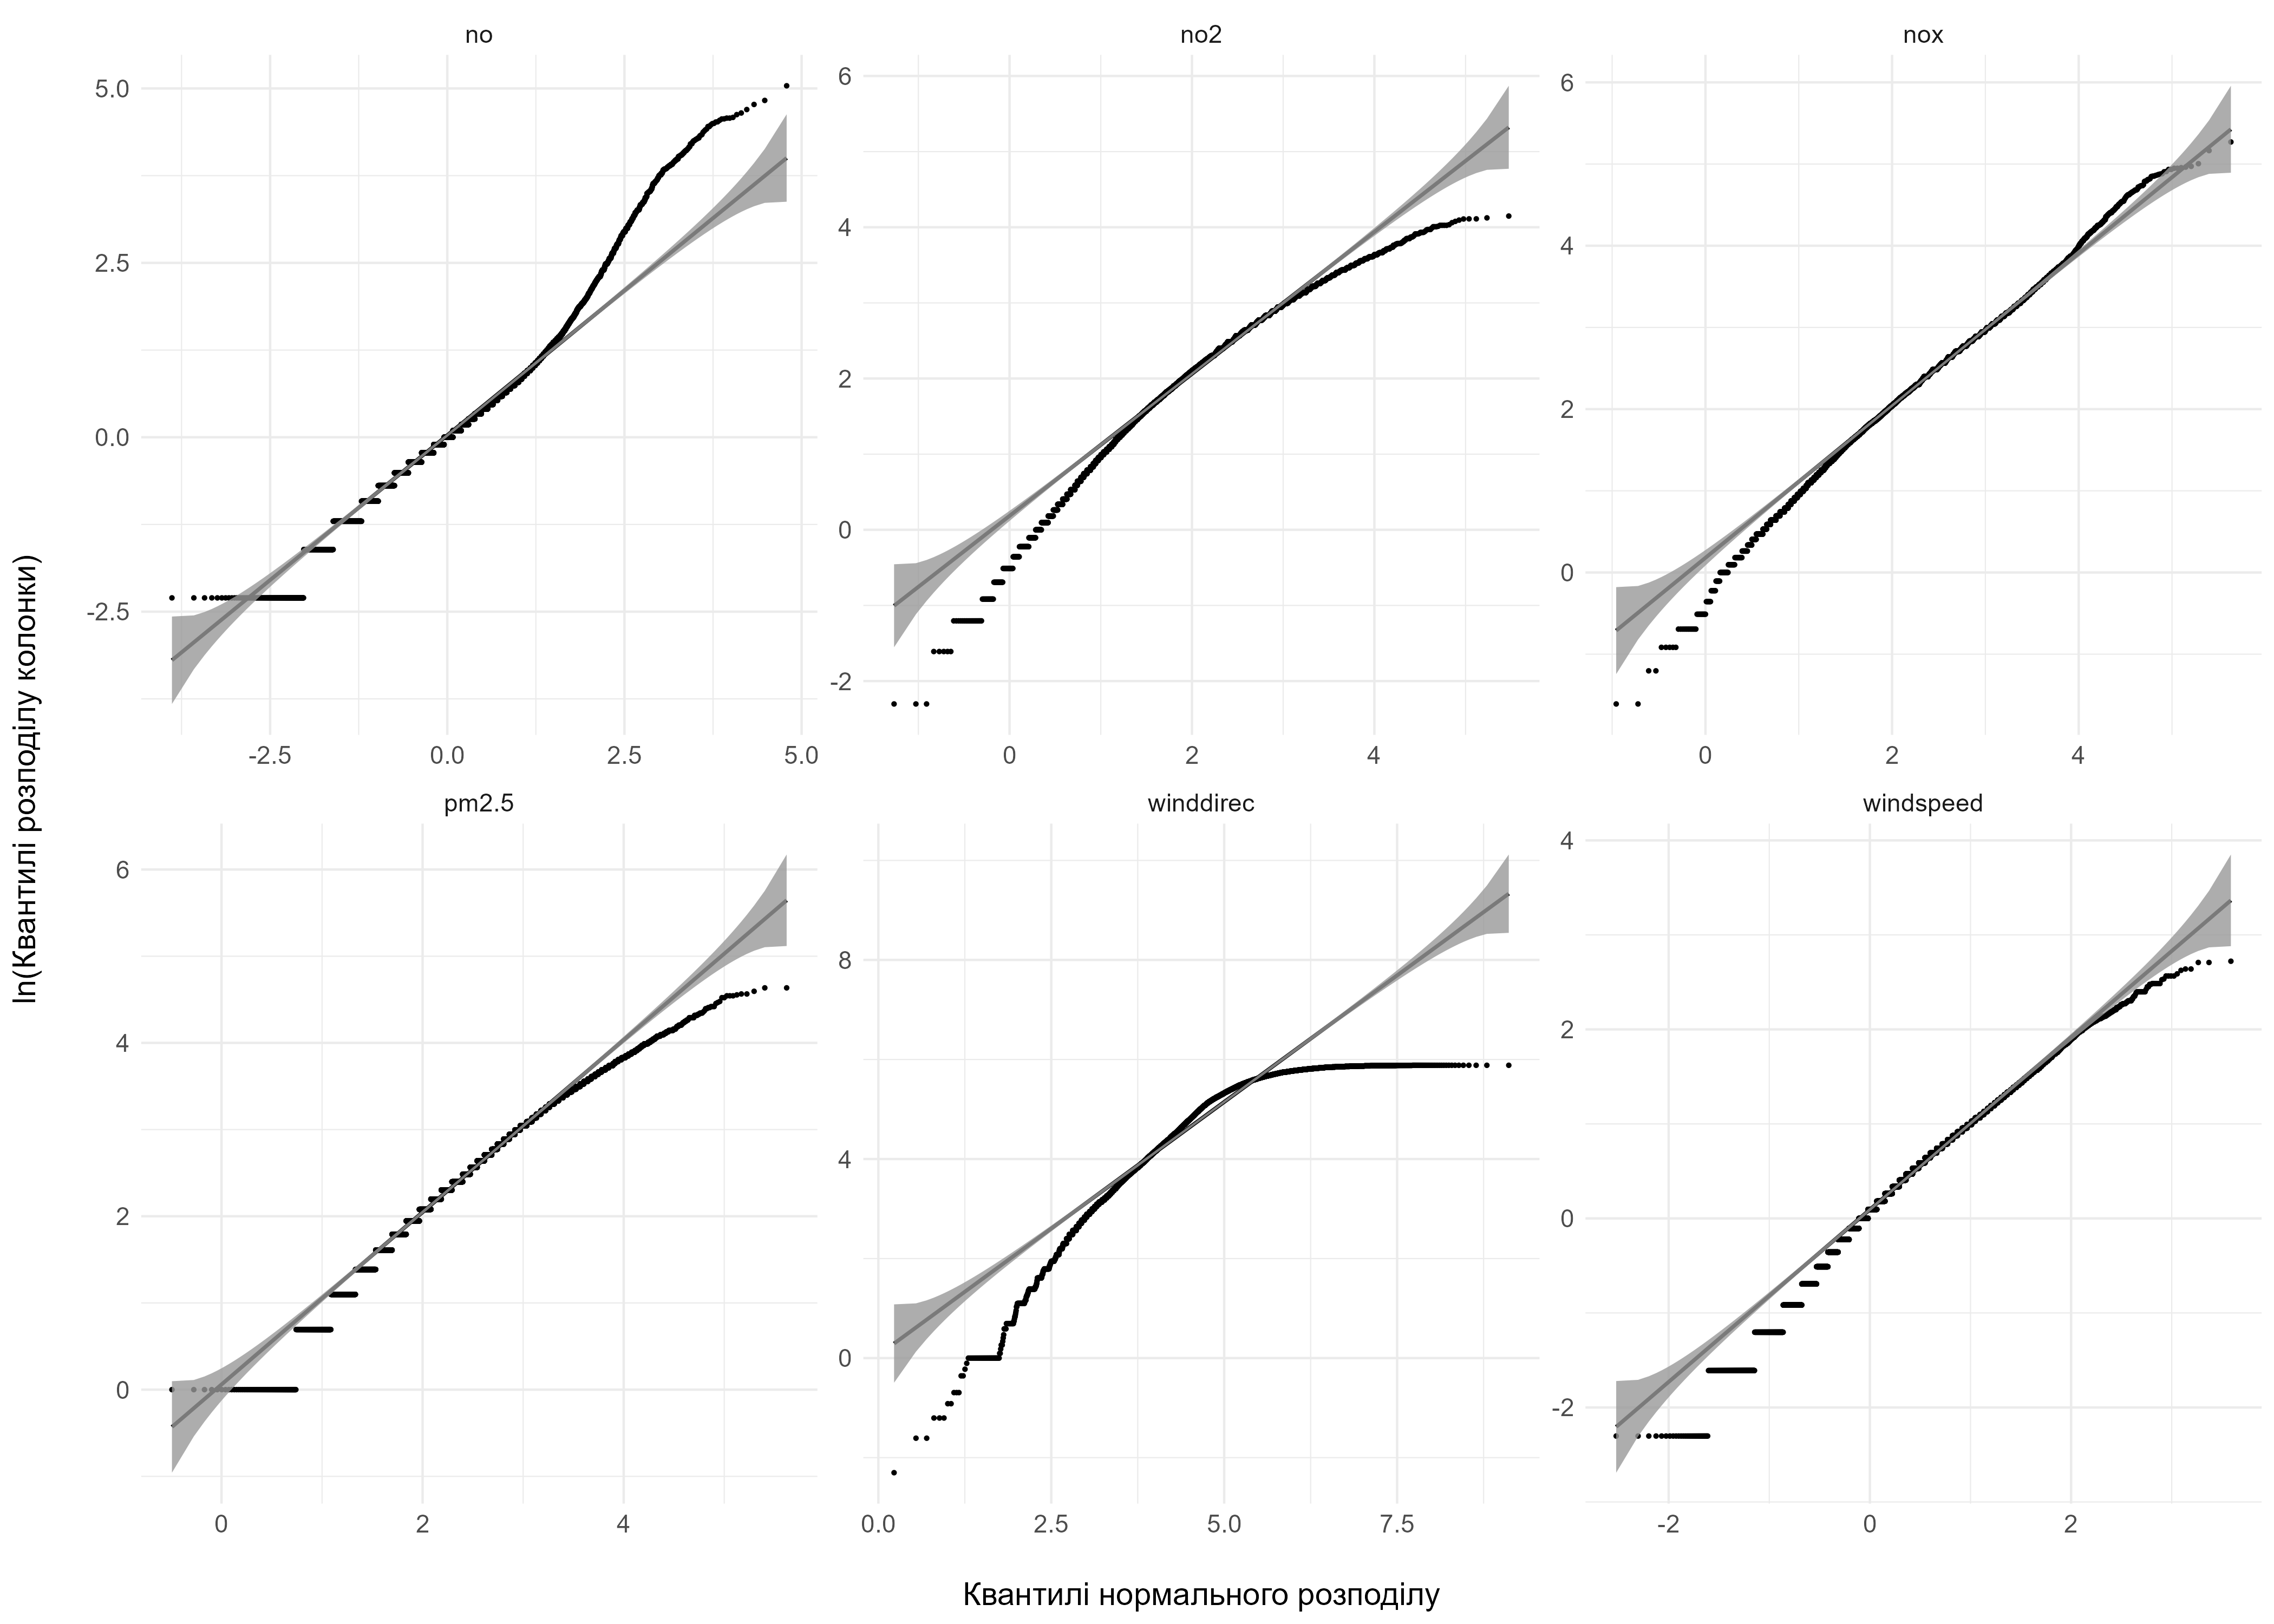
\includegraphics[height=3in]{plots/qq_tidy/qq-log-p2.png}
  \end{center}
\end{frame}

\begin{frame}
  \section{Питання EDA}

  \frametitle{Зміст}
  \tableofcontents[currentsection]
\end{frame}

%% Question 1

\begin{frame}
  \frametitle{Чи впливає швидкість вітру на концентрацію частинок PM2.5 і PM10}

  \quad \textit{Був використаний trimmed набір даних}

  \begin{tabular}{cc}
    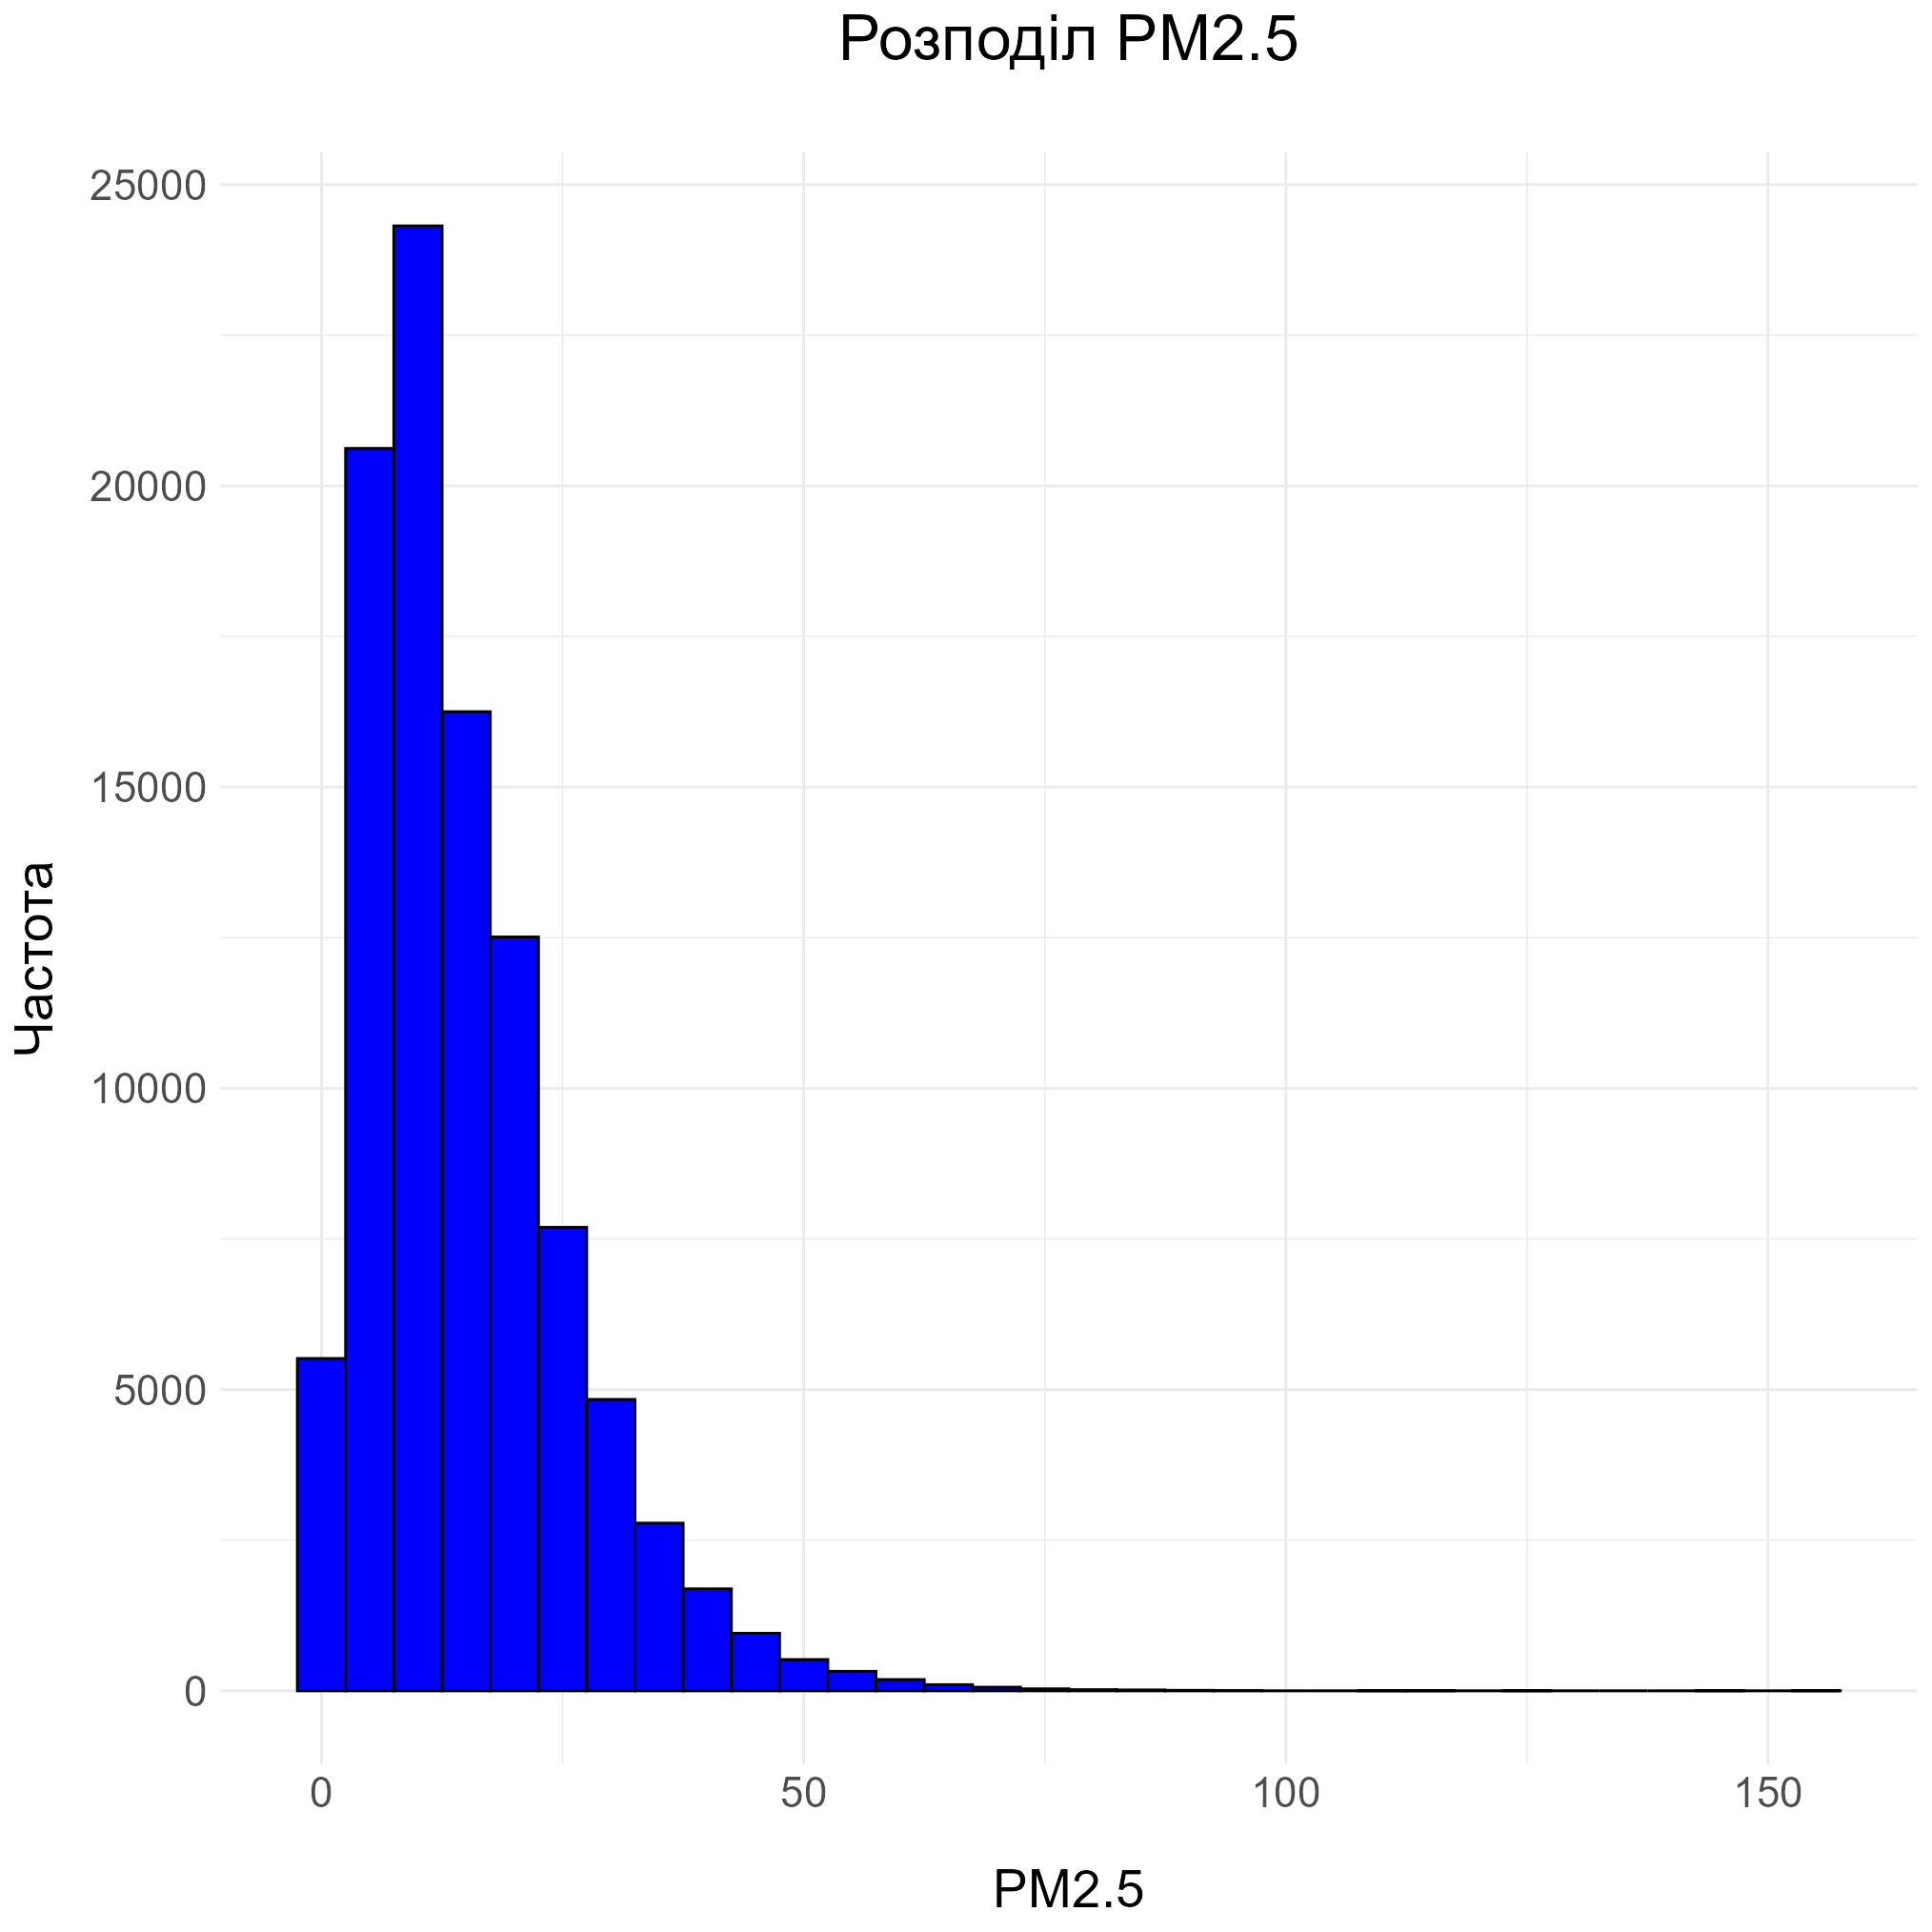
\includegraphics[height=2.2in]{plots/question1/pm2_5_gist.png} &
    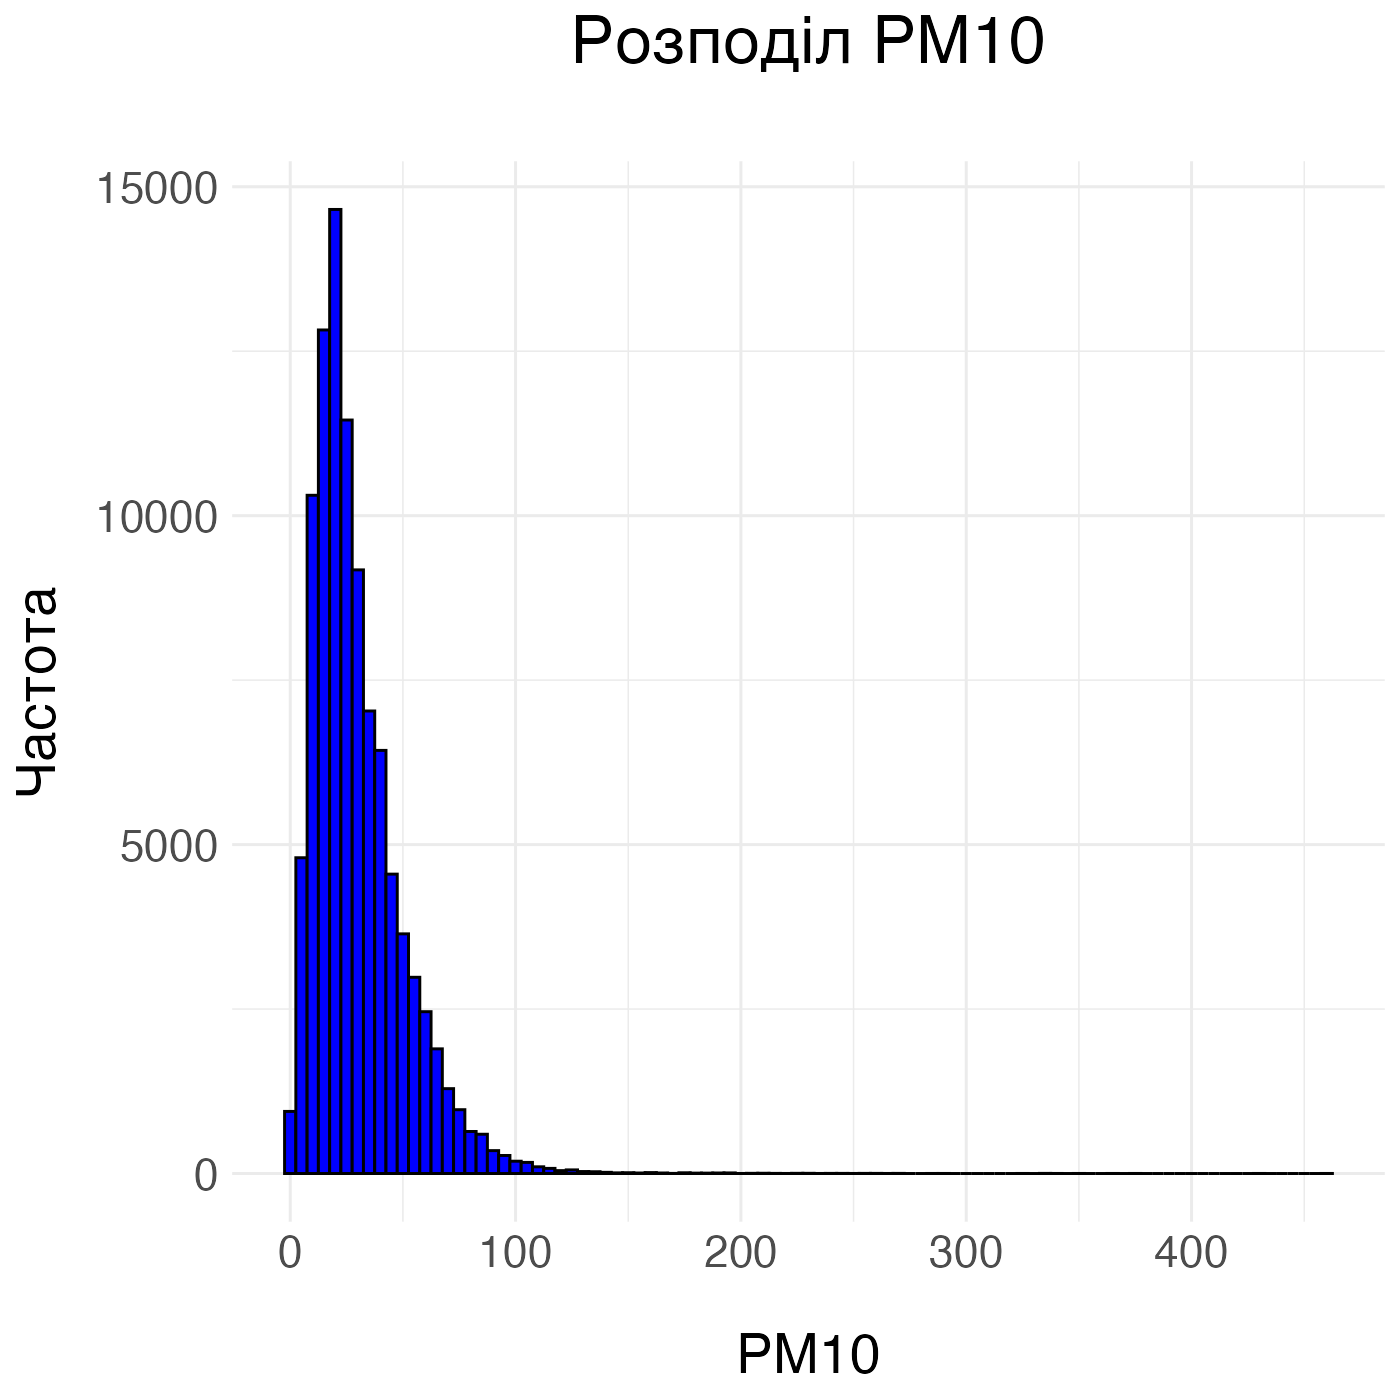
\includegraphics[height=2.2in]{plots/question1/pm10_gist.png}
  \end{tabular}
\end{frame}

\begin{frame}
  \frametitle{Чи впливає швидкість вітру на концентрацію частинок PM2.5 і PM10}

  \begin{tabular}{cc}
    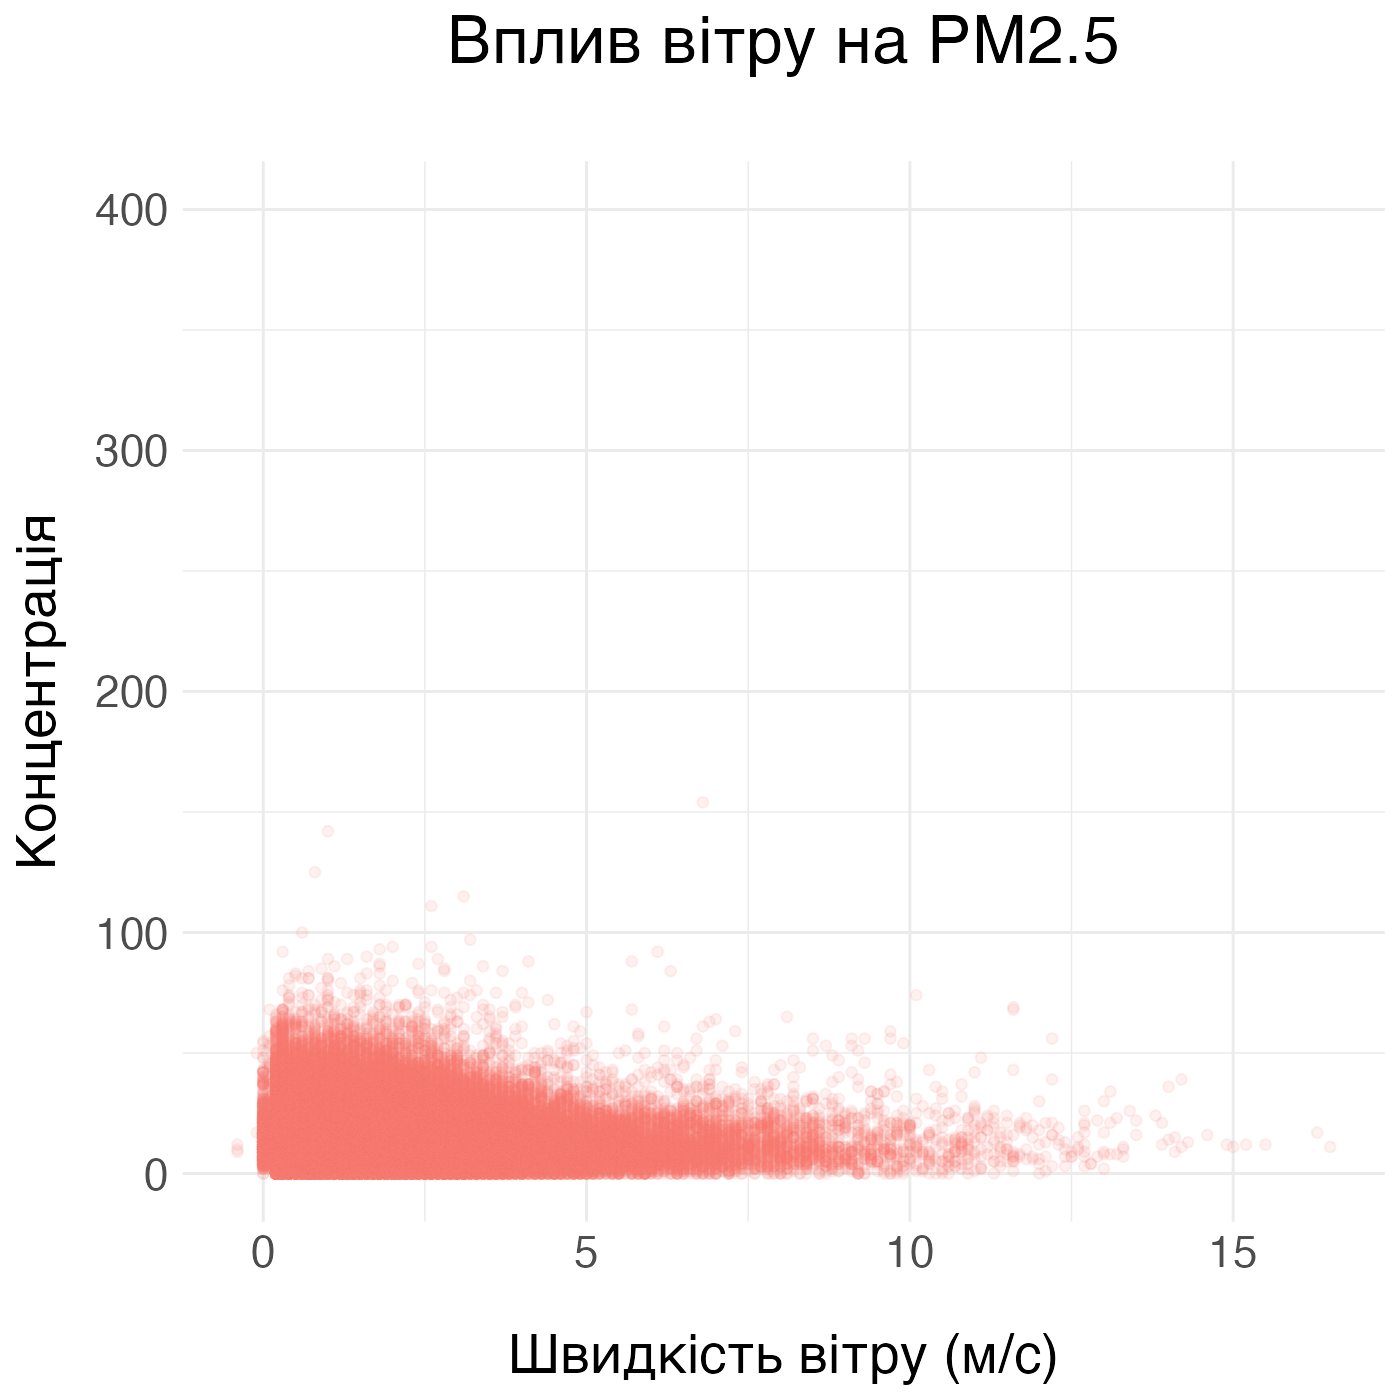
\includegraphics[height=2.2in]{plots/question1/wind_speed_vs_pm2_5.png} &
    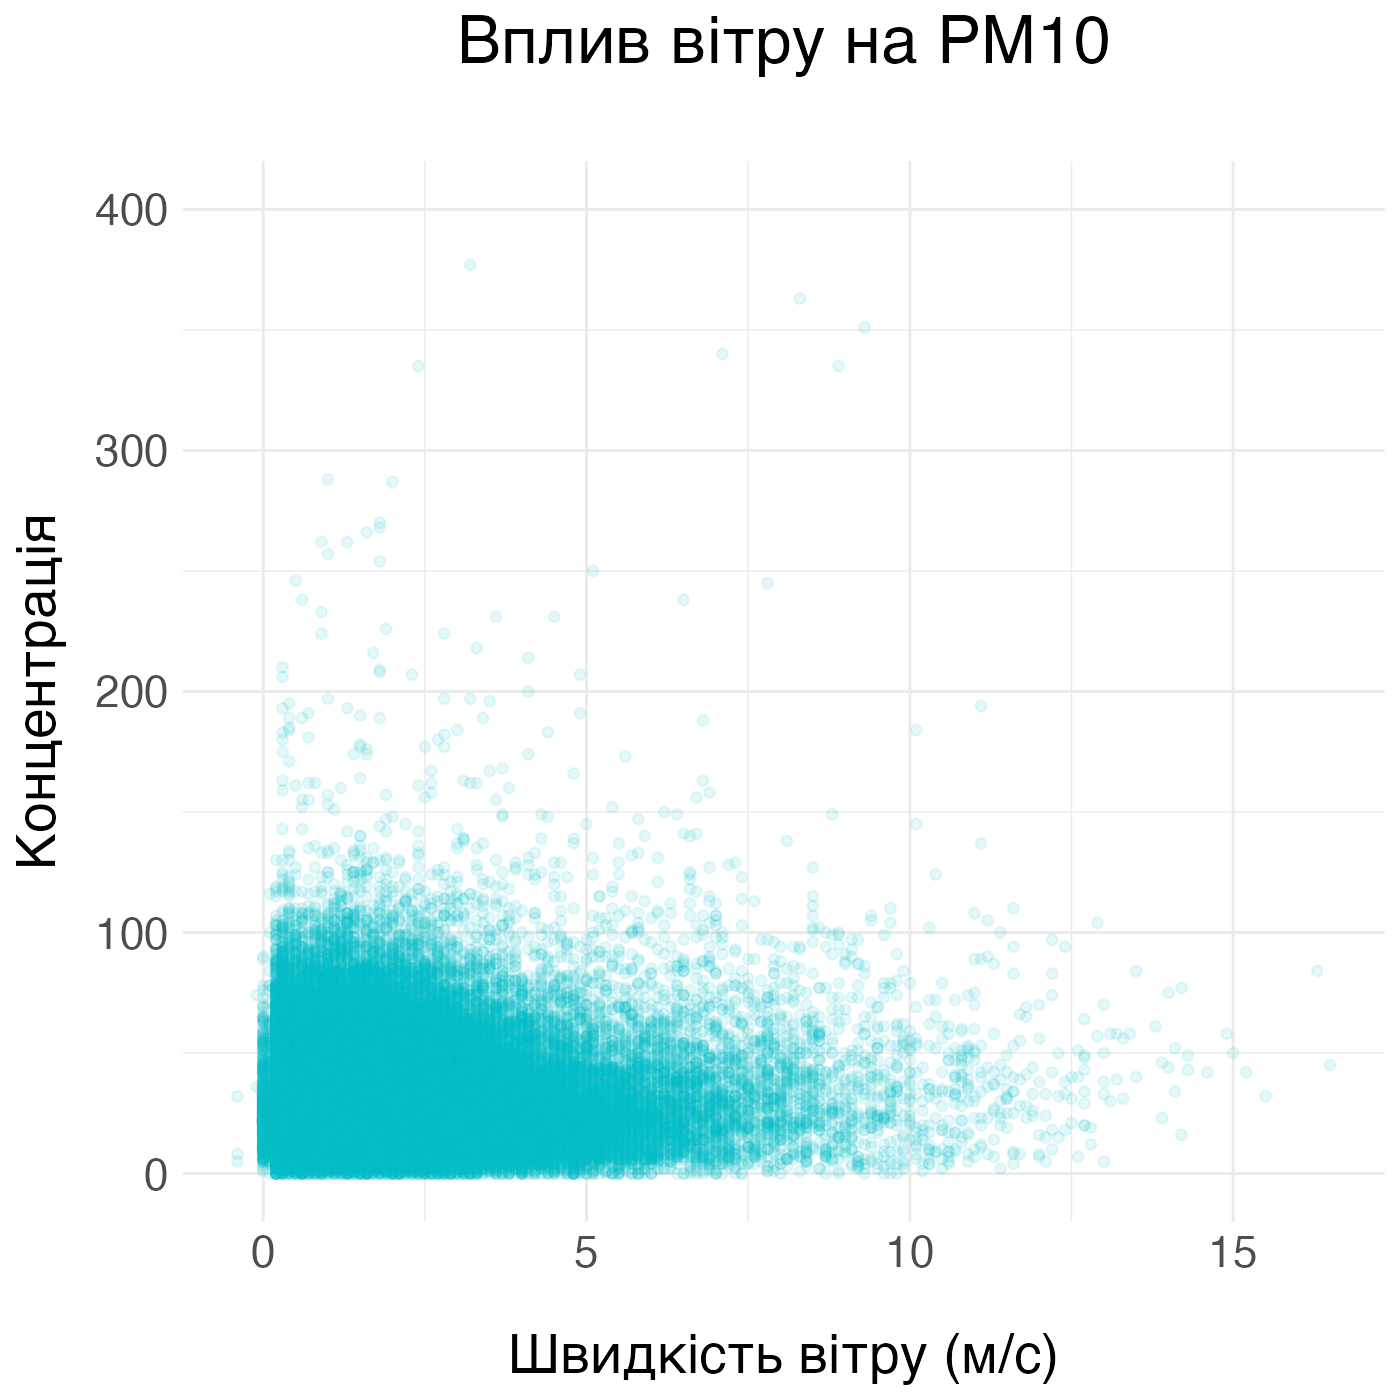
\includegraphics[height=2.2in]{plots/question1/wind_speed_vs_pm10.png}
  \end{tabular}
\end{frame}

\begin{frame}
  \frametitle{Чи впливає швидкість вітру на концентрацію частинок PM2.5 і PM10}

  \begin{tabular}{cc}
    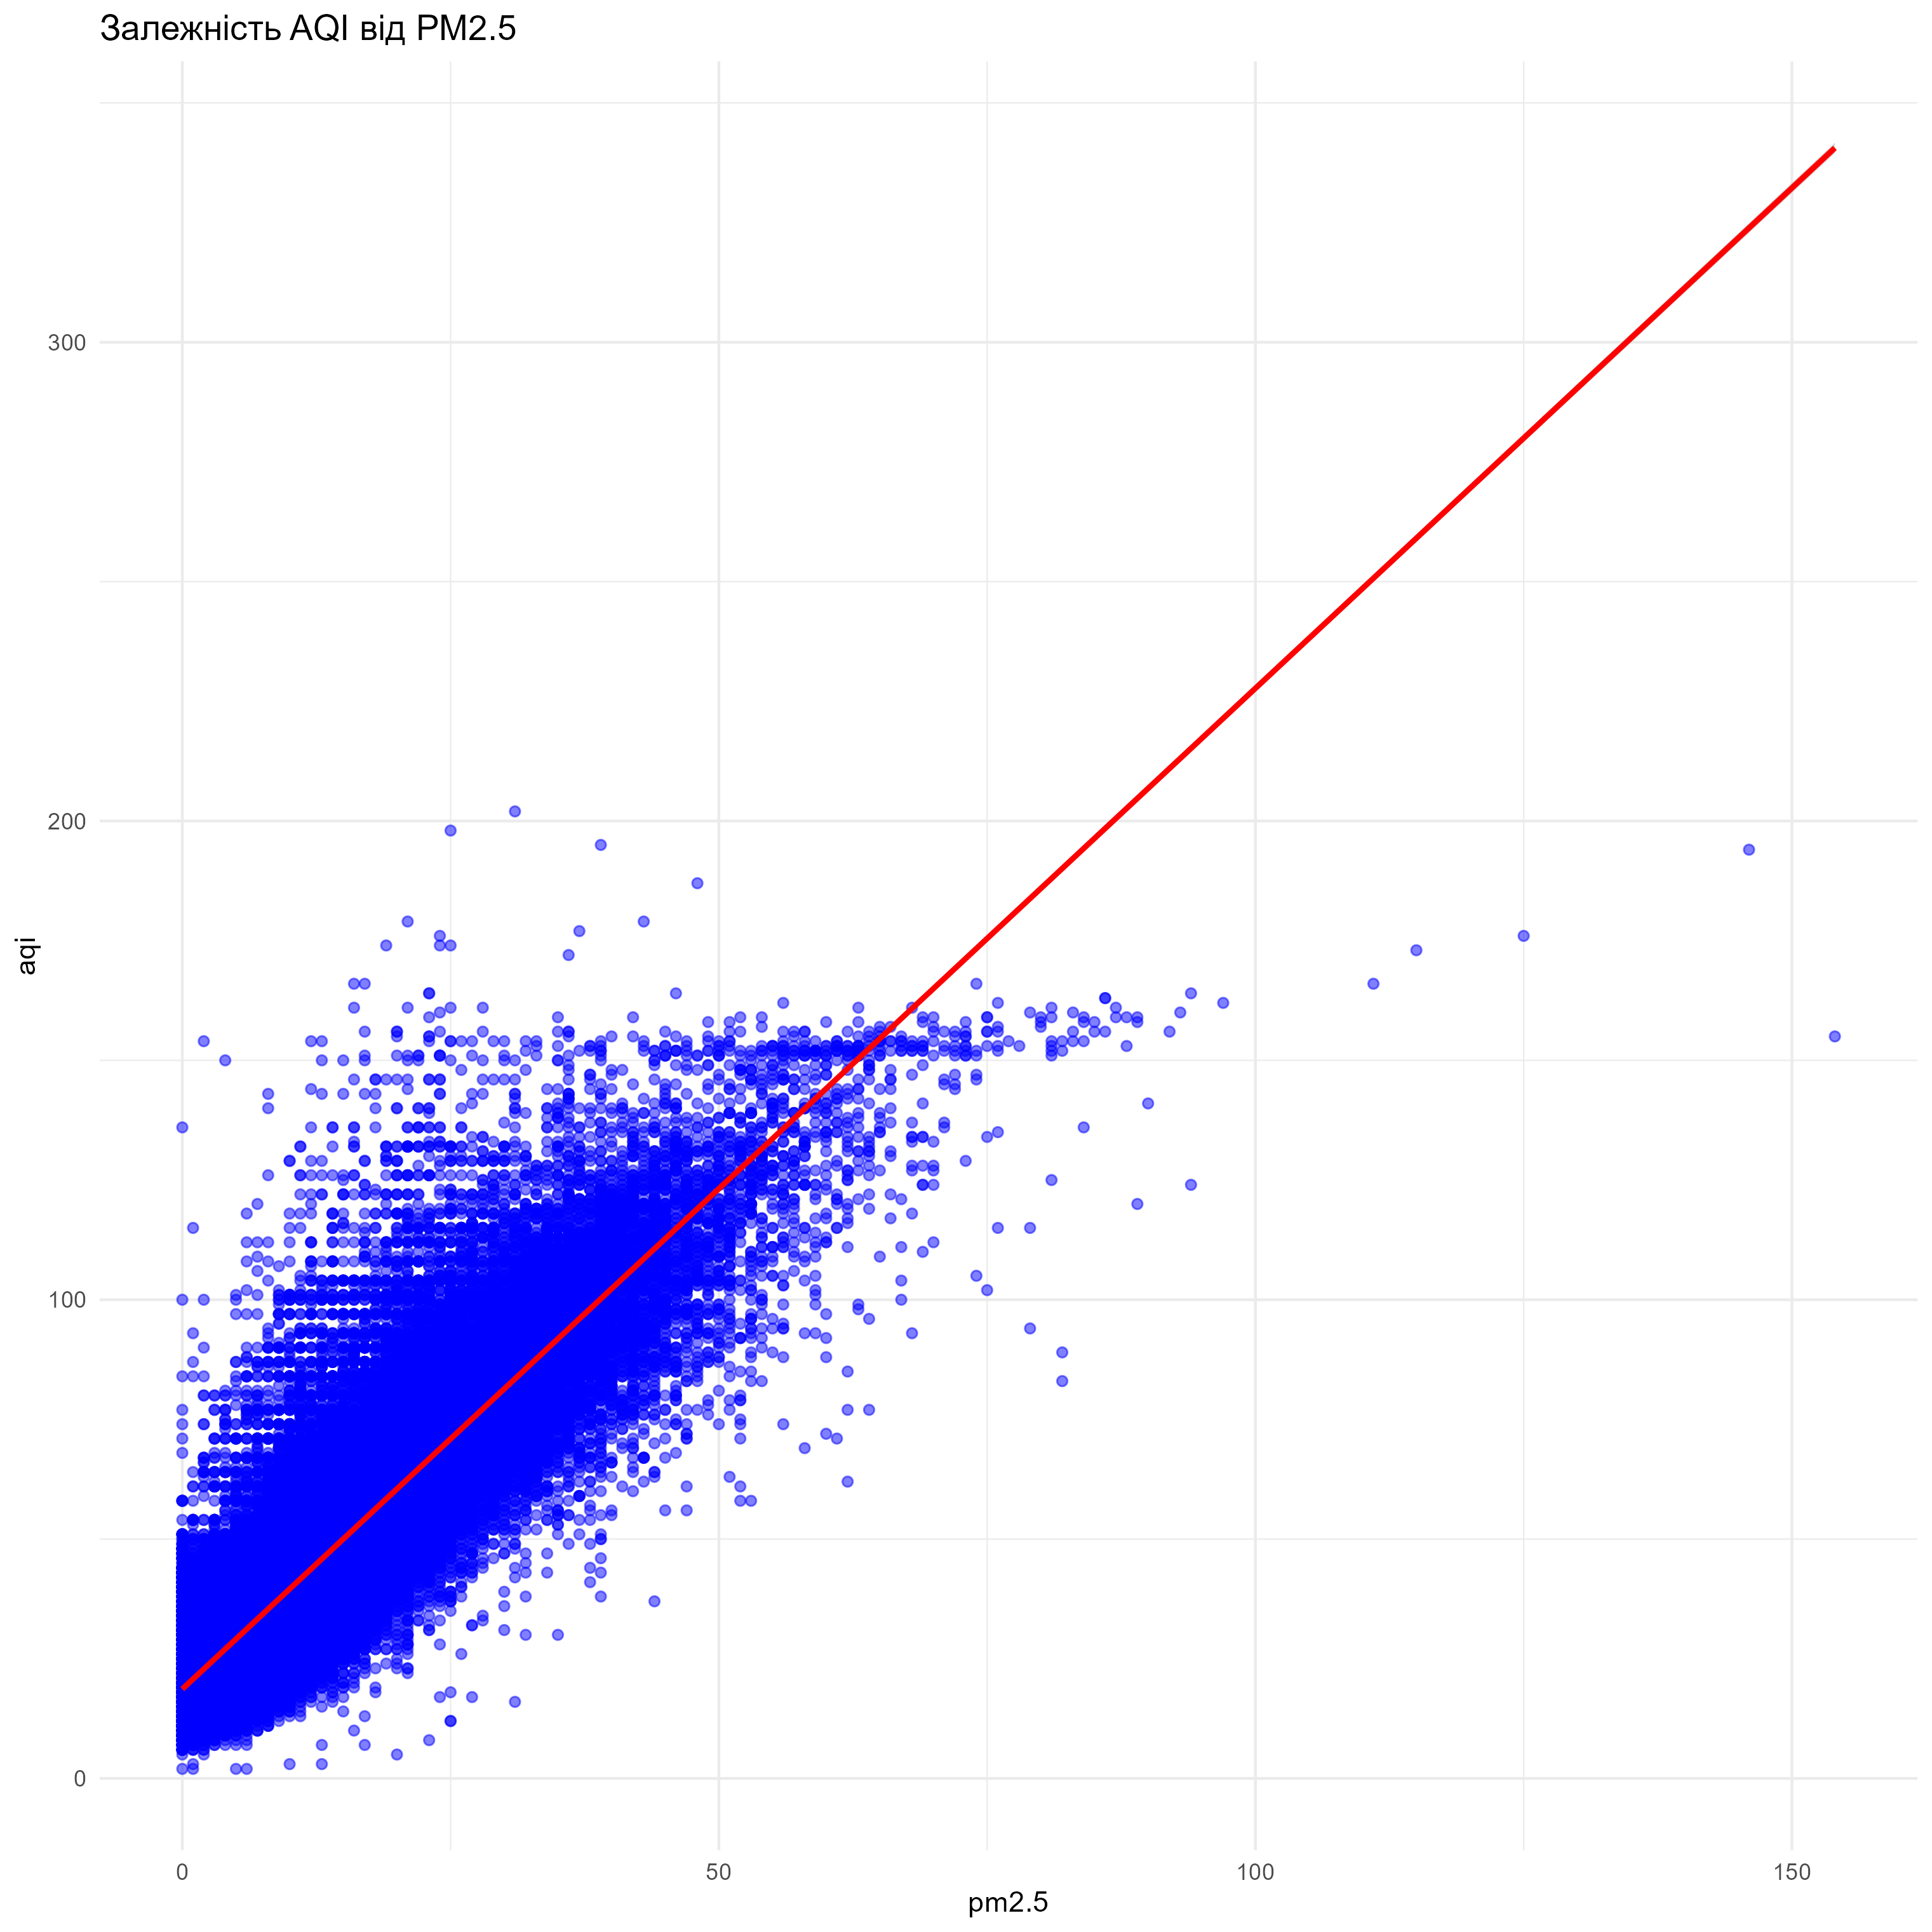
\includegraphics[height=2.2in]{plots/question1/aqi_pm2_5_diagram.png} &
    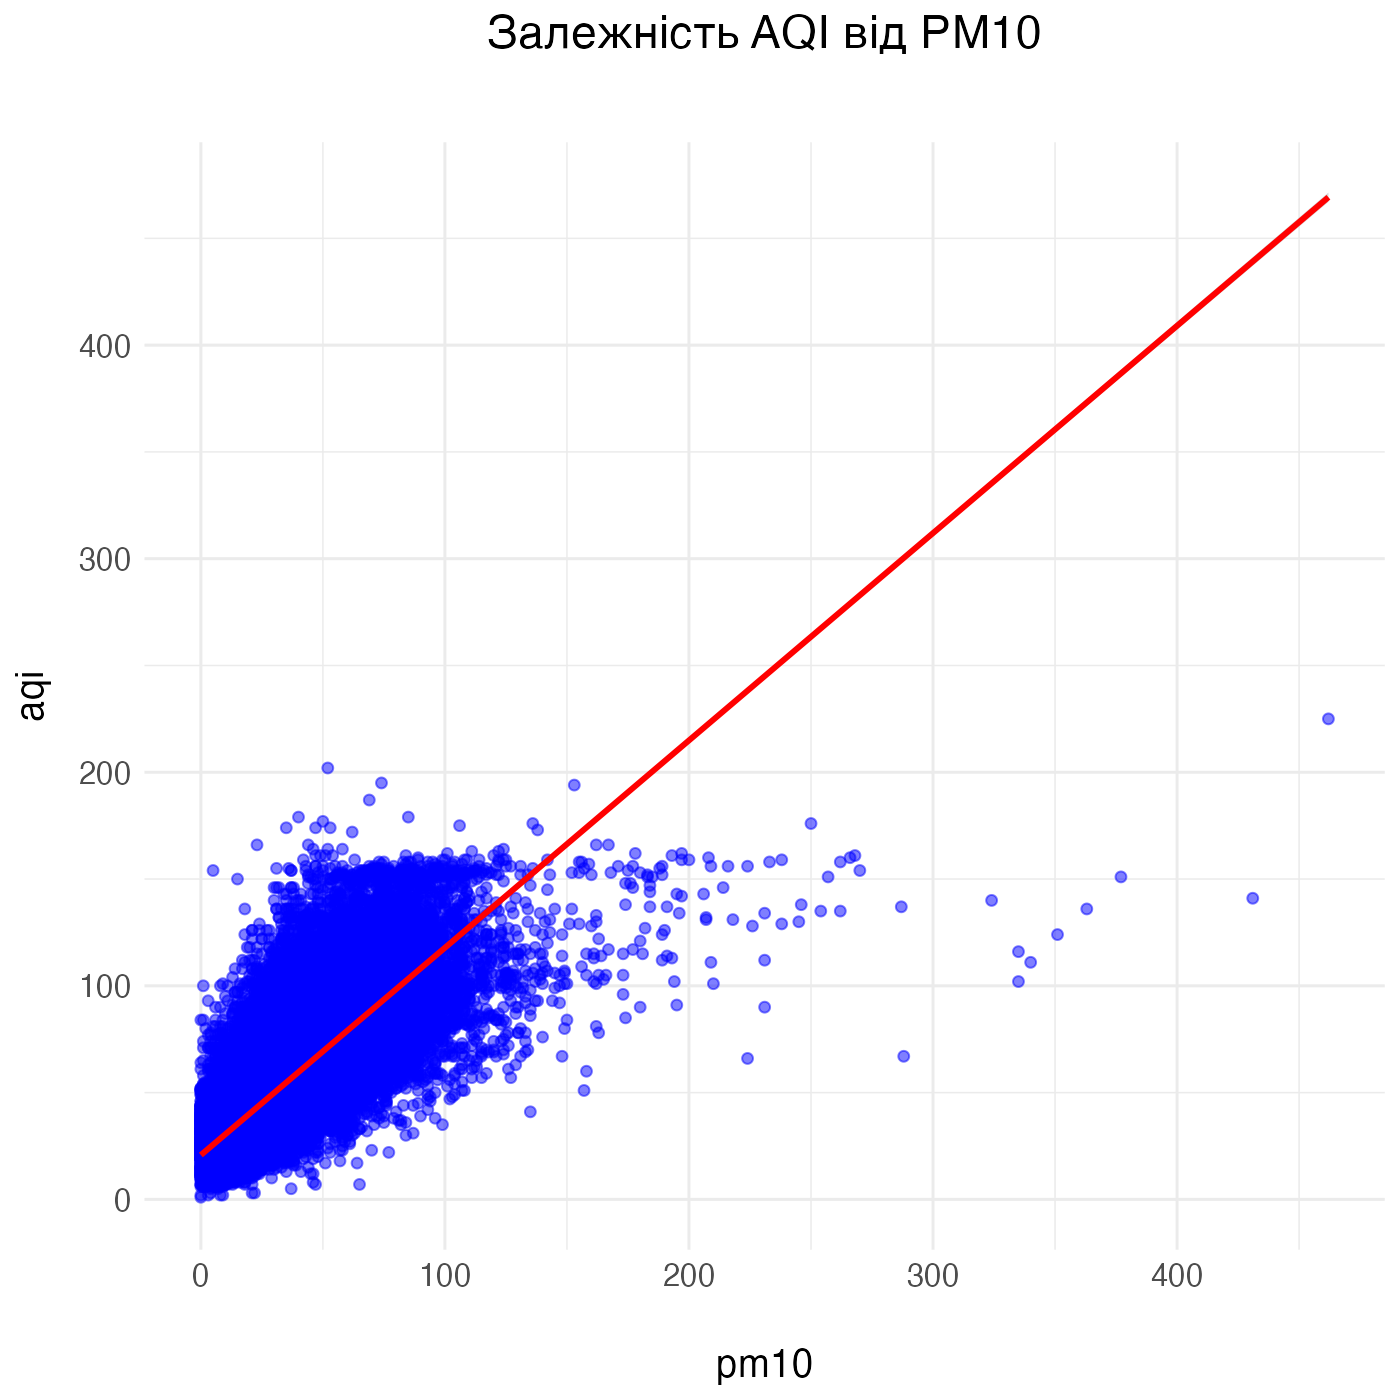
\includegraphics[height=2.2in]{plots/question1/aqi_pm10_diagram.png}
  \end{tabular}
\end{frame}

\begin{frame}
  \frametitle{Чи впливає швидкість вітру на концентрацію частинок PM2.5 і PM10}

  \begin{center}
    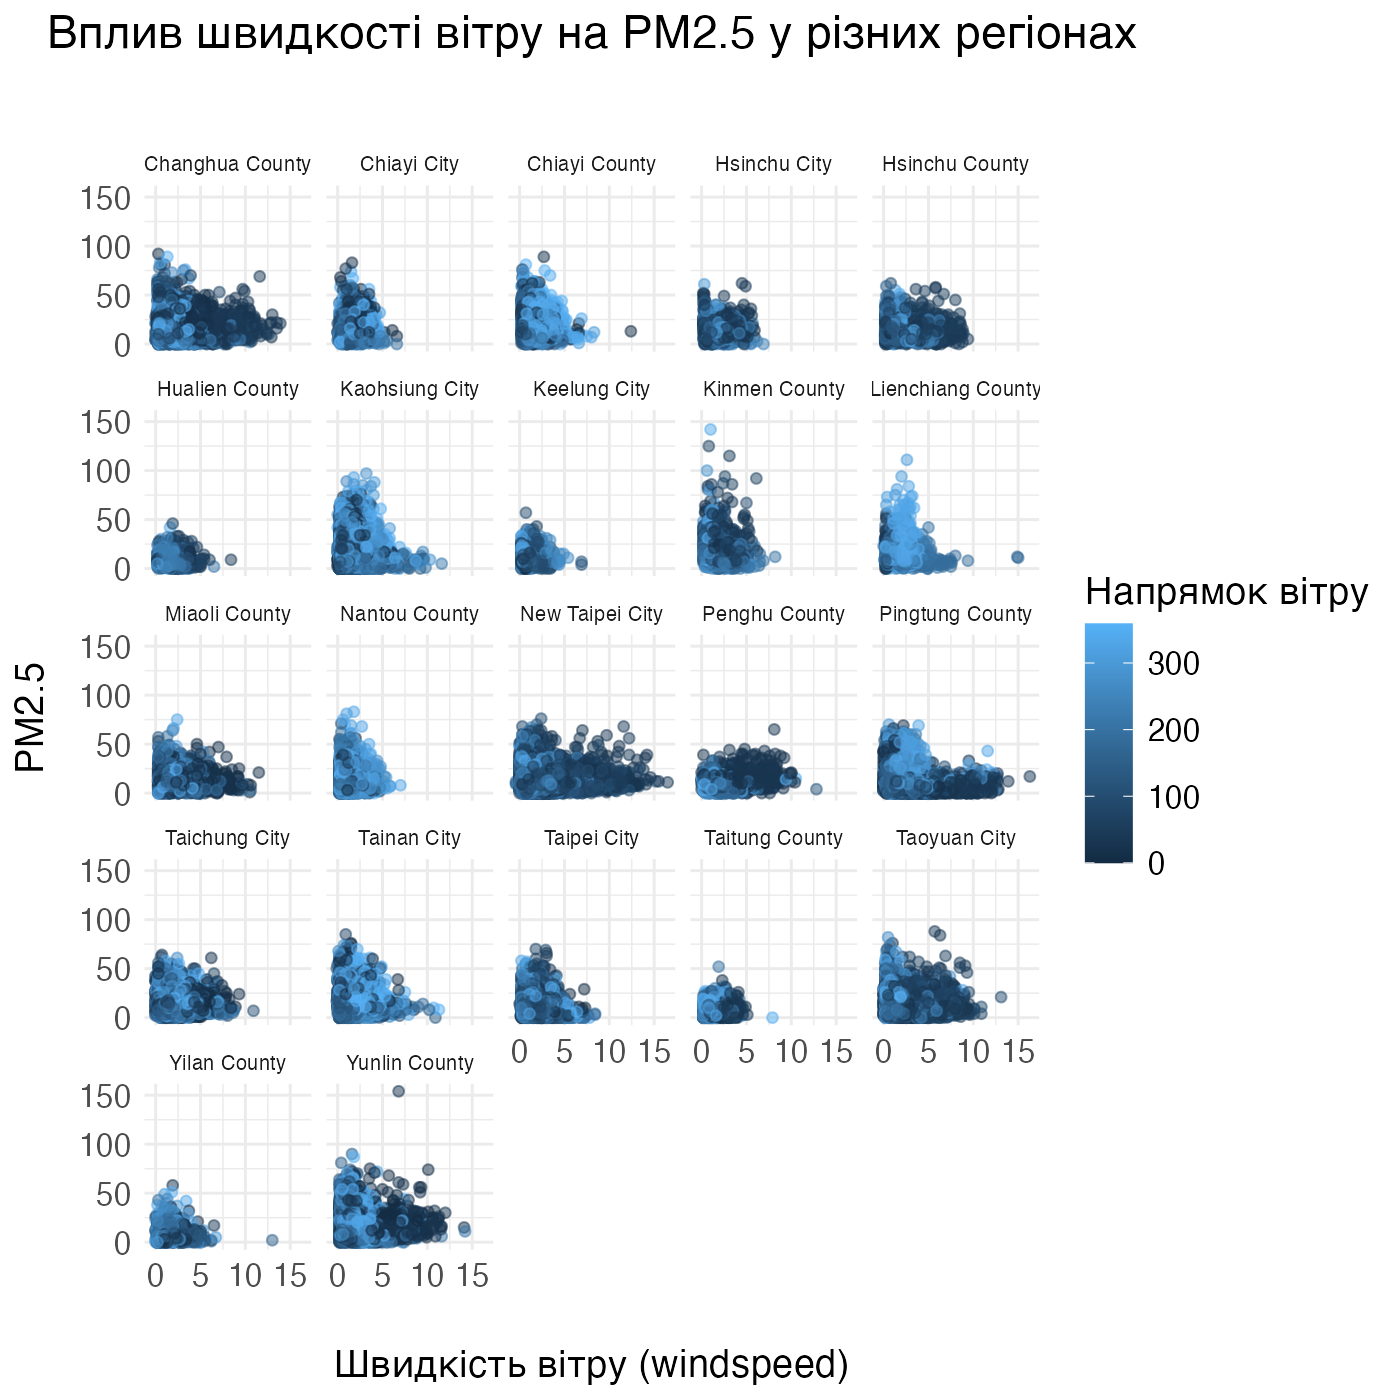
\includegraphics[height=2.8in]{plots/question1/scatter_pm2_5_region.png}
  \end{center}
\end{frame}

\begin{frame}
  \frametitle{Чи впливає швидкість вітру на концентрацію частинок PM2.5 і PM10}

  \begin{center}
    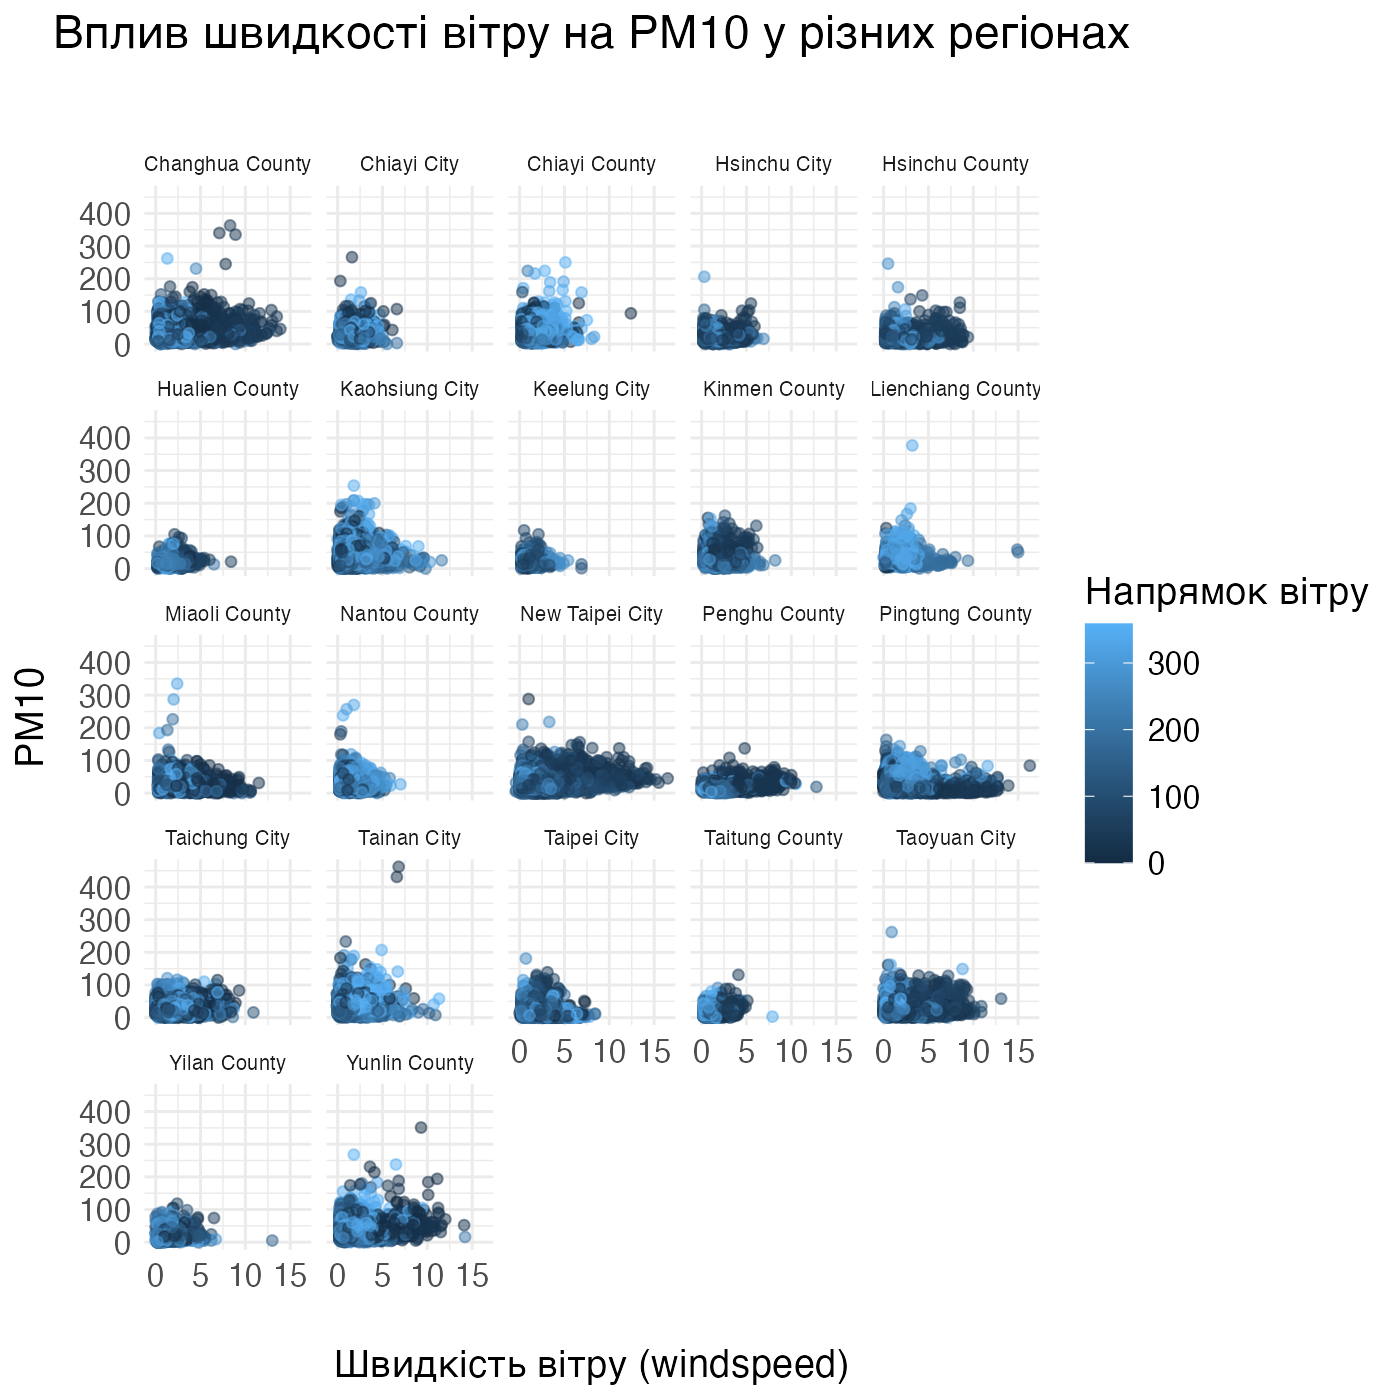
\includegraphics[height=2.8in]{plots/question1/scatter_pm10_region.png}
  \end{center}
\end{frame}

\begin{frame}
  \frametitle{Чи впливає швидкість вітру на концентрацію частинок PM2.5 і PM10}

  \begin{center}
    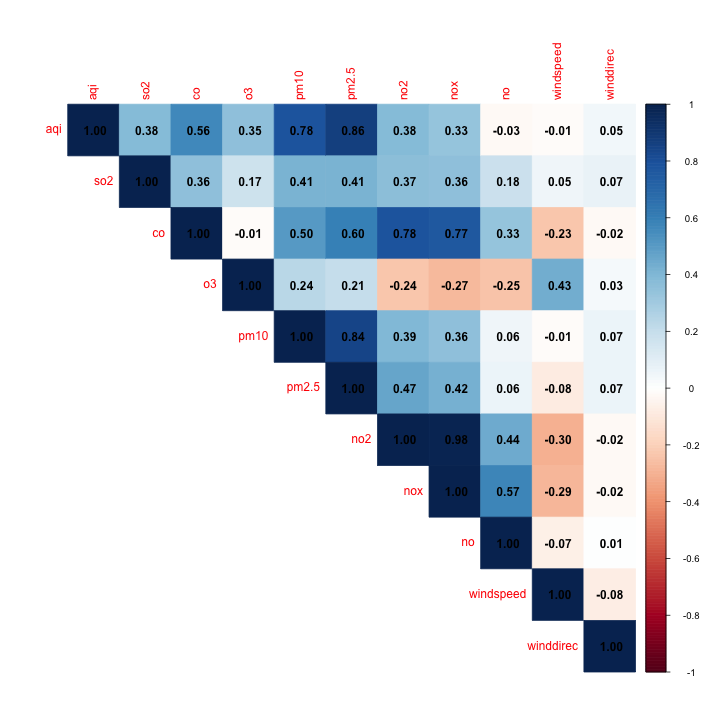
\includegraphics[height=2.8in]{plots/question1/corr_matrix_plot.png}
  \end{center}
\end{frame}

\begin{frame}
  \frametitle{Чи впливає швидкість вітру на концентрацію частинок PM2.5 і PM10}

  \begin{enumerate}
    \item Підсумовуючи можна сказати, що $PM_{2.5}$ і $ PM_{10}$ слабко негативно корелюють зі швидкістю вітру.
    \item Проте вплив вітру на газоподібні забруднювачі ($NO_2$, $NO_x$) є сильнішим. 
    Це може бути через більшу мобільність газів у порівнянні з твердими частинками.
  \end{enumerate}

\end{frame}

%% Question 2

\begin{frame}
  \frametitle{Як зміни в концентрації $O_3$ та $SO_2$ впливають на загальний рівень забруднення повітря (AQI)?}

  \textit{Був використаний trimmed набір даних}

  Аналіз викидів та розподілу всіх показників забруднення:

  \begin{center}
    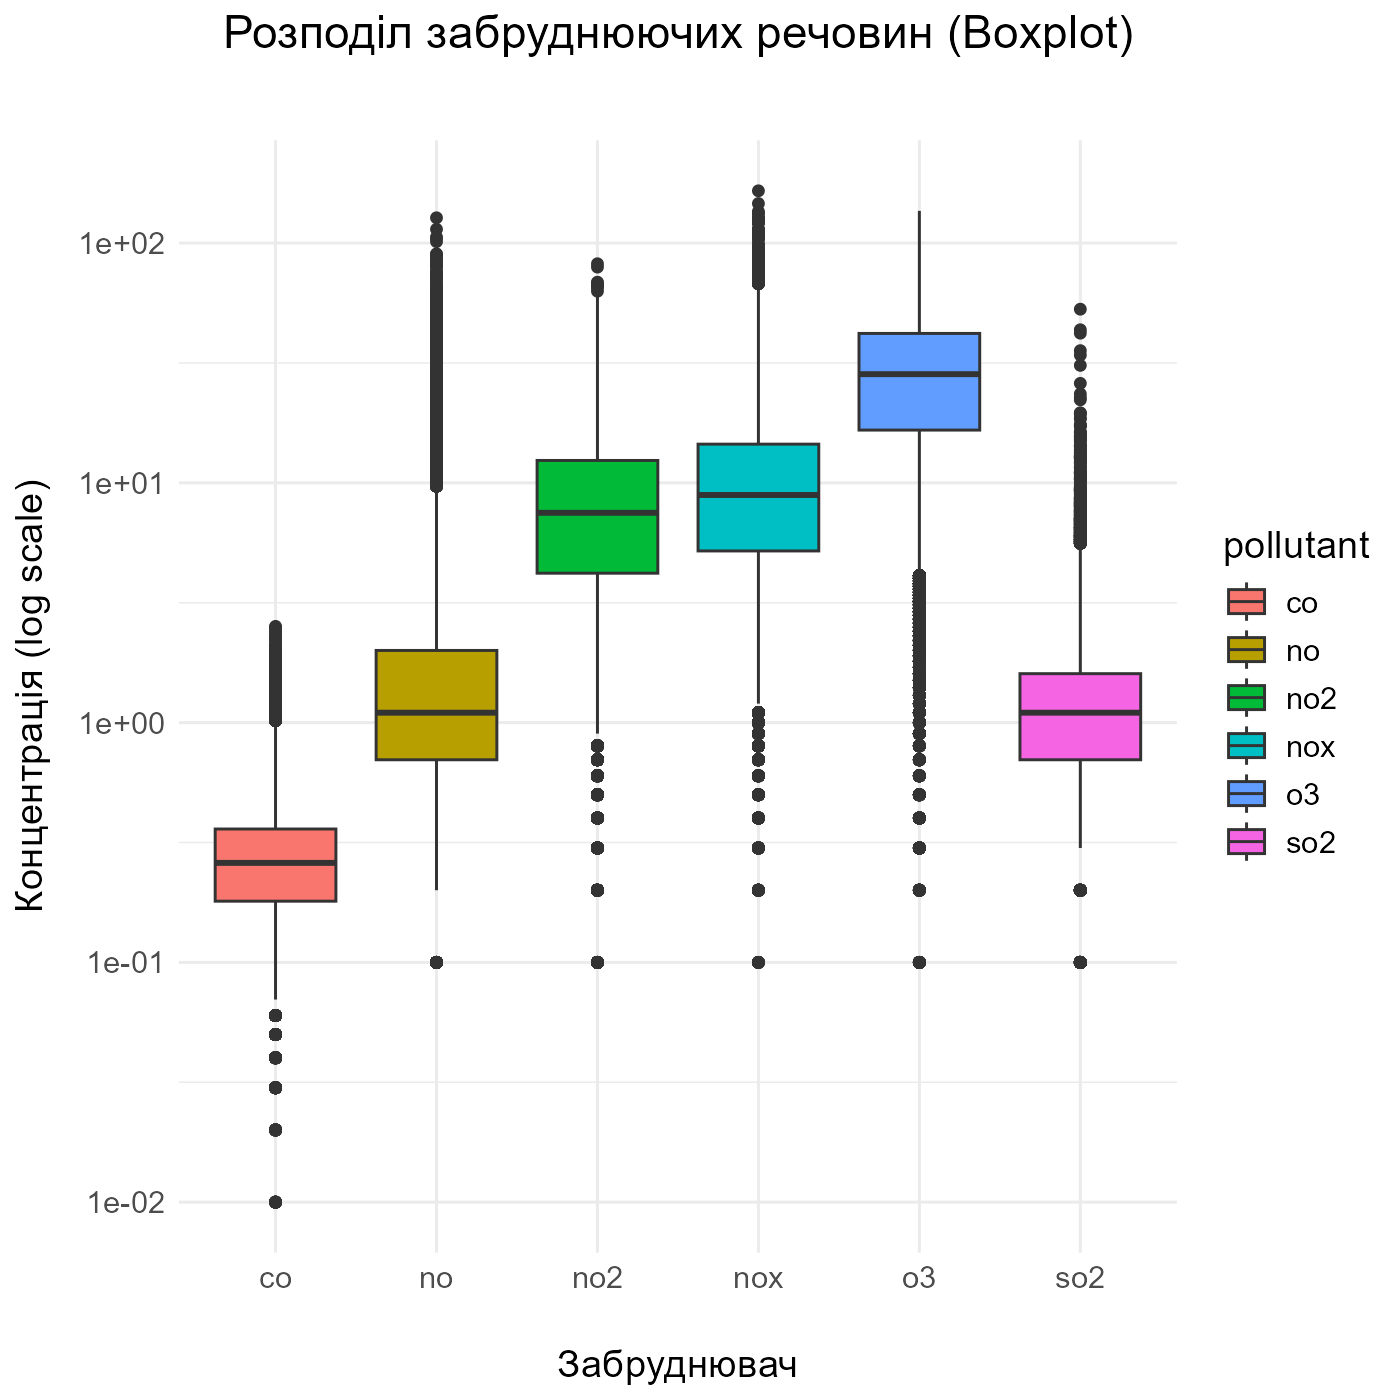
\includegraphics[height=2in]{plots/question2/boxplot_pollutants.png}
  \end{center}
\end{frame}

\begin{frame}
  \frametitle{Як зміни в концентрації $O_3$ та $SO_2$ впливають на загальний рівень забруднення повітря (AQI)?}
  
  \begin{center}
    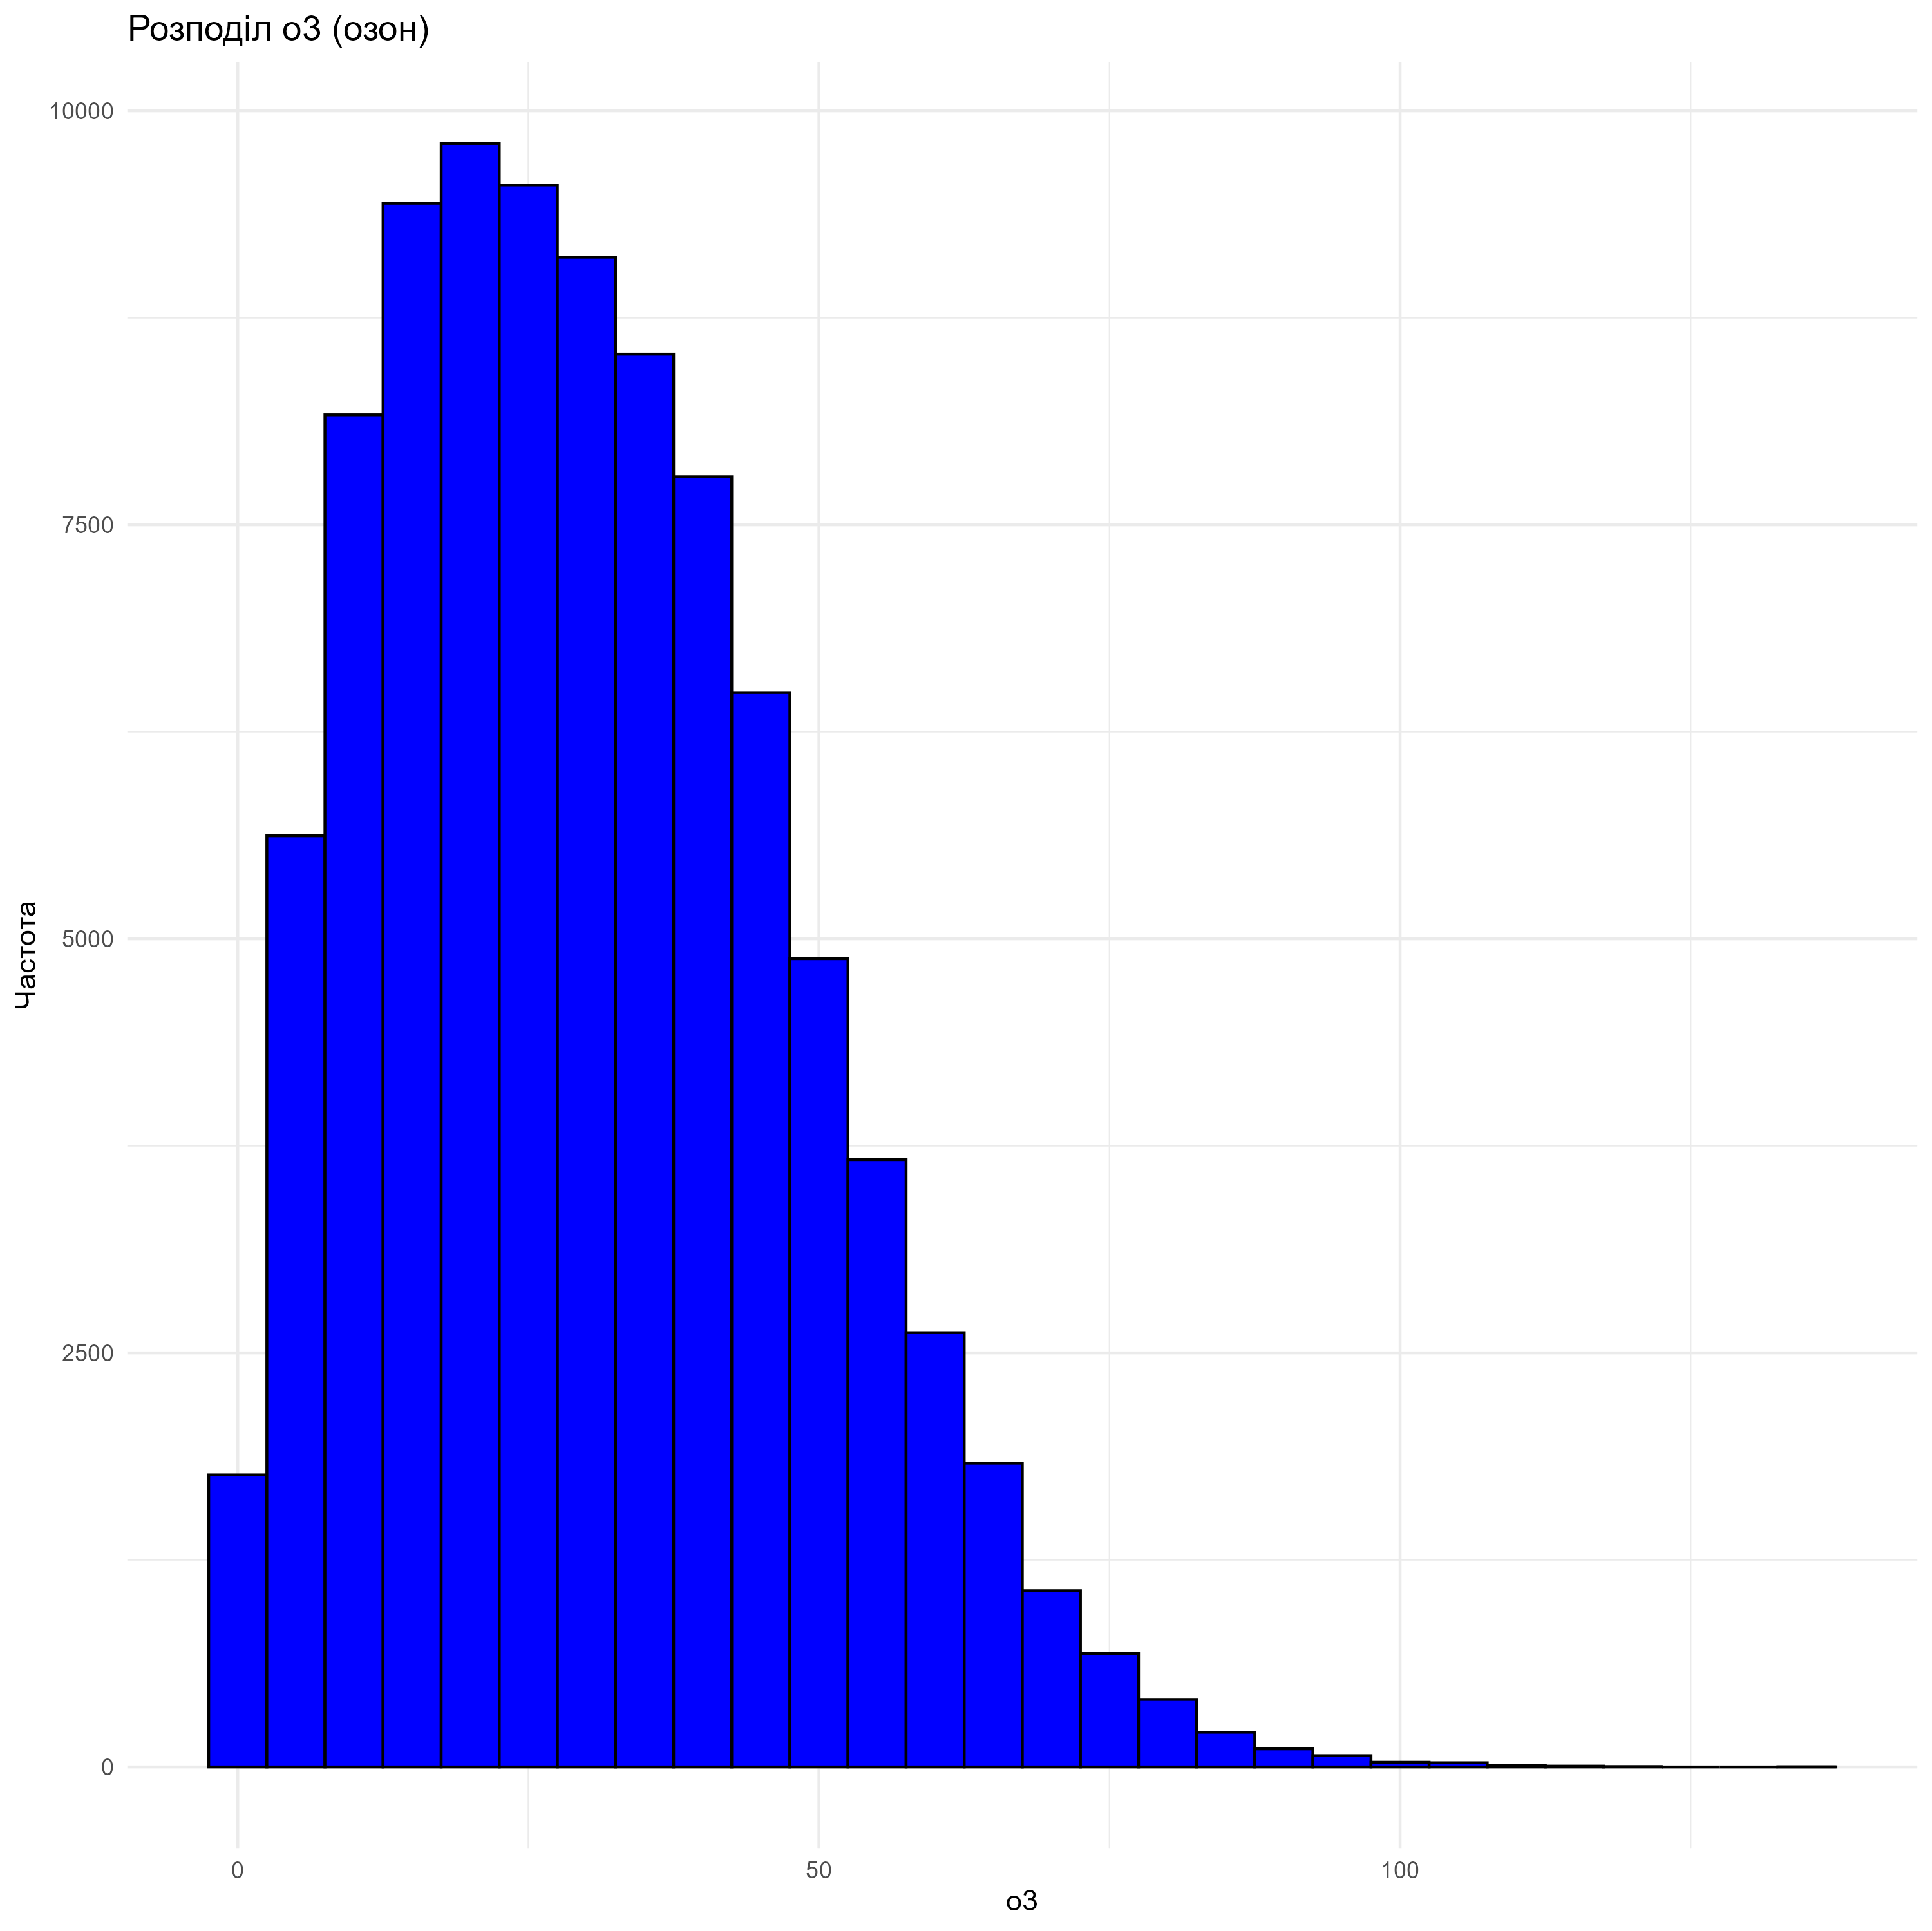
\includegraphics[height=2.8in]{plots/question2/o3_plot.png}
  \end{center}
\end{frame}

\begin{frame}
  \frametitle{Як зміни в концентрації $O_3$ та $SO_2$ впливають на загальний рівень забруднення повітря (AQI)?}

  \begin{center}
    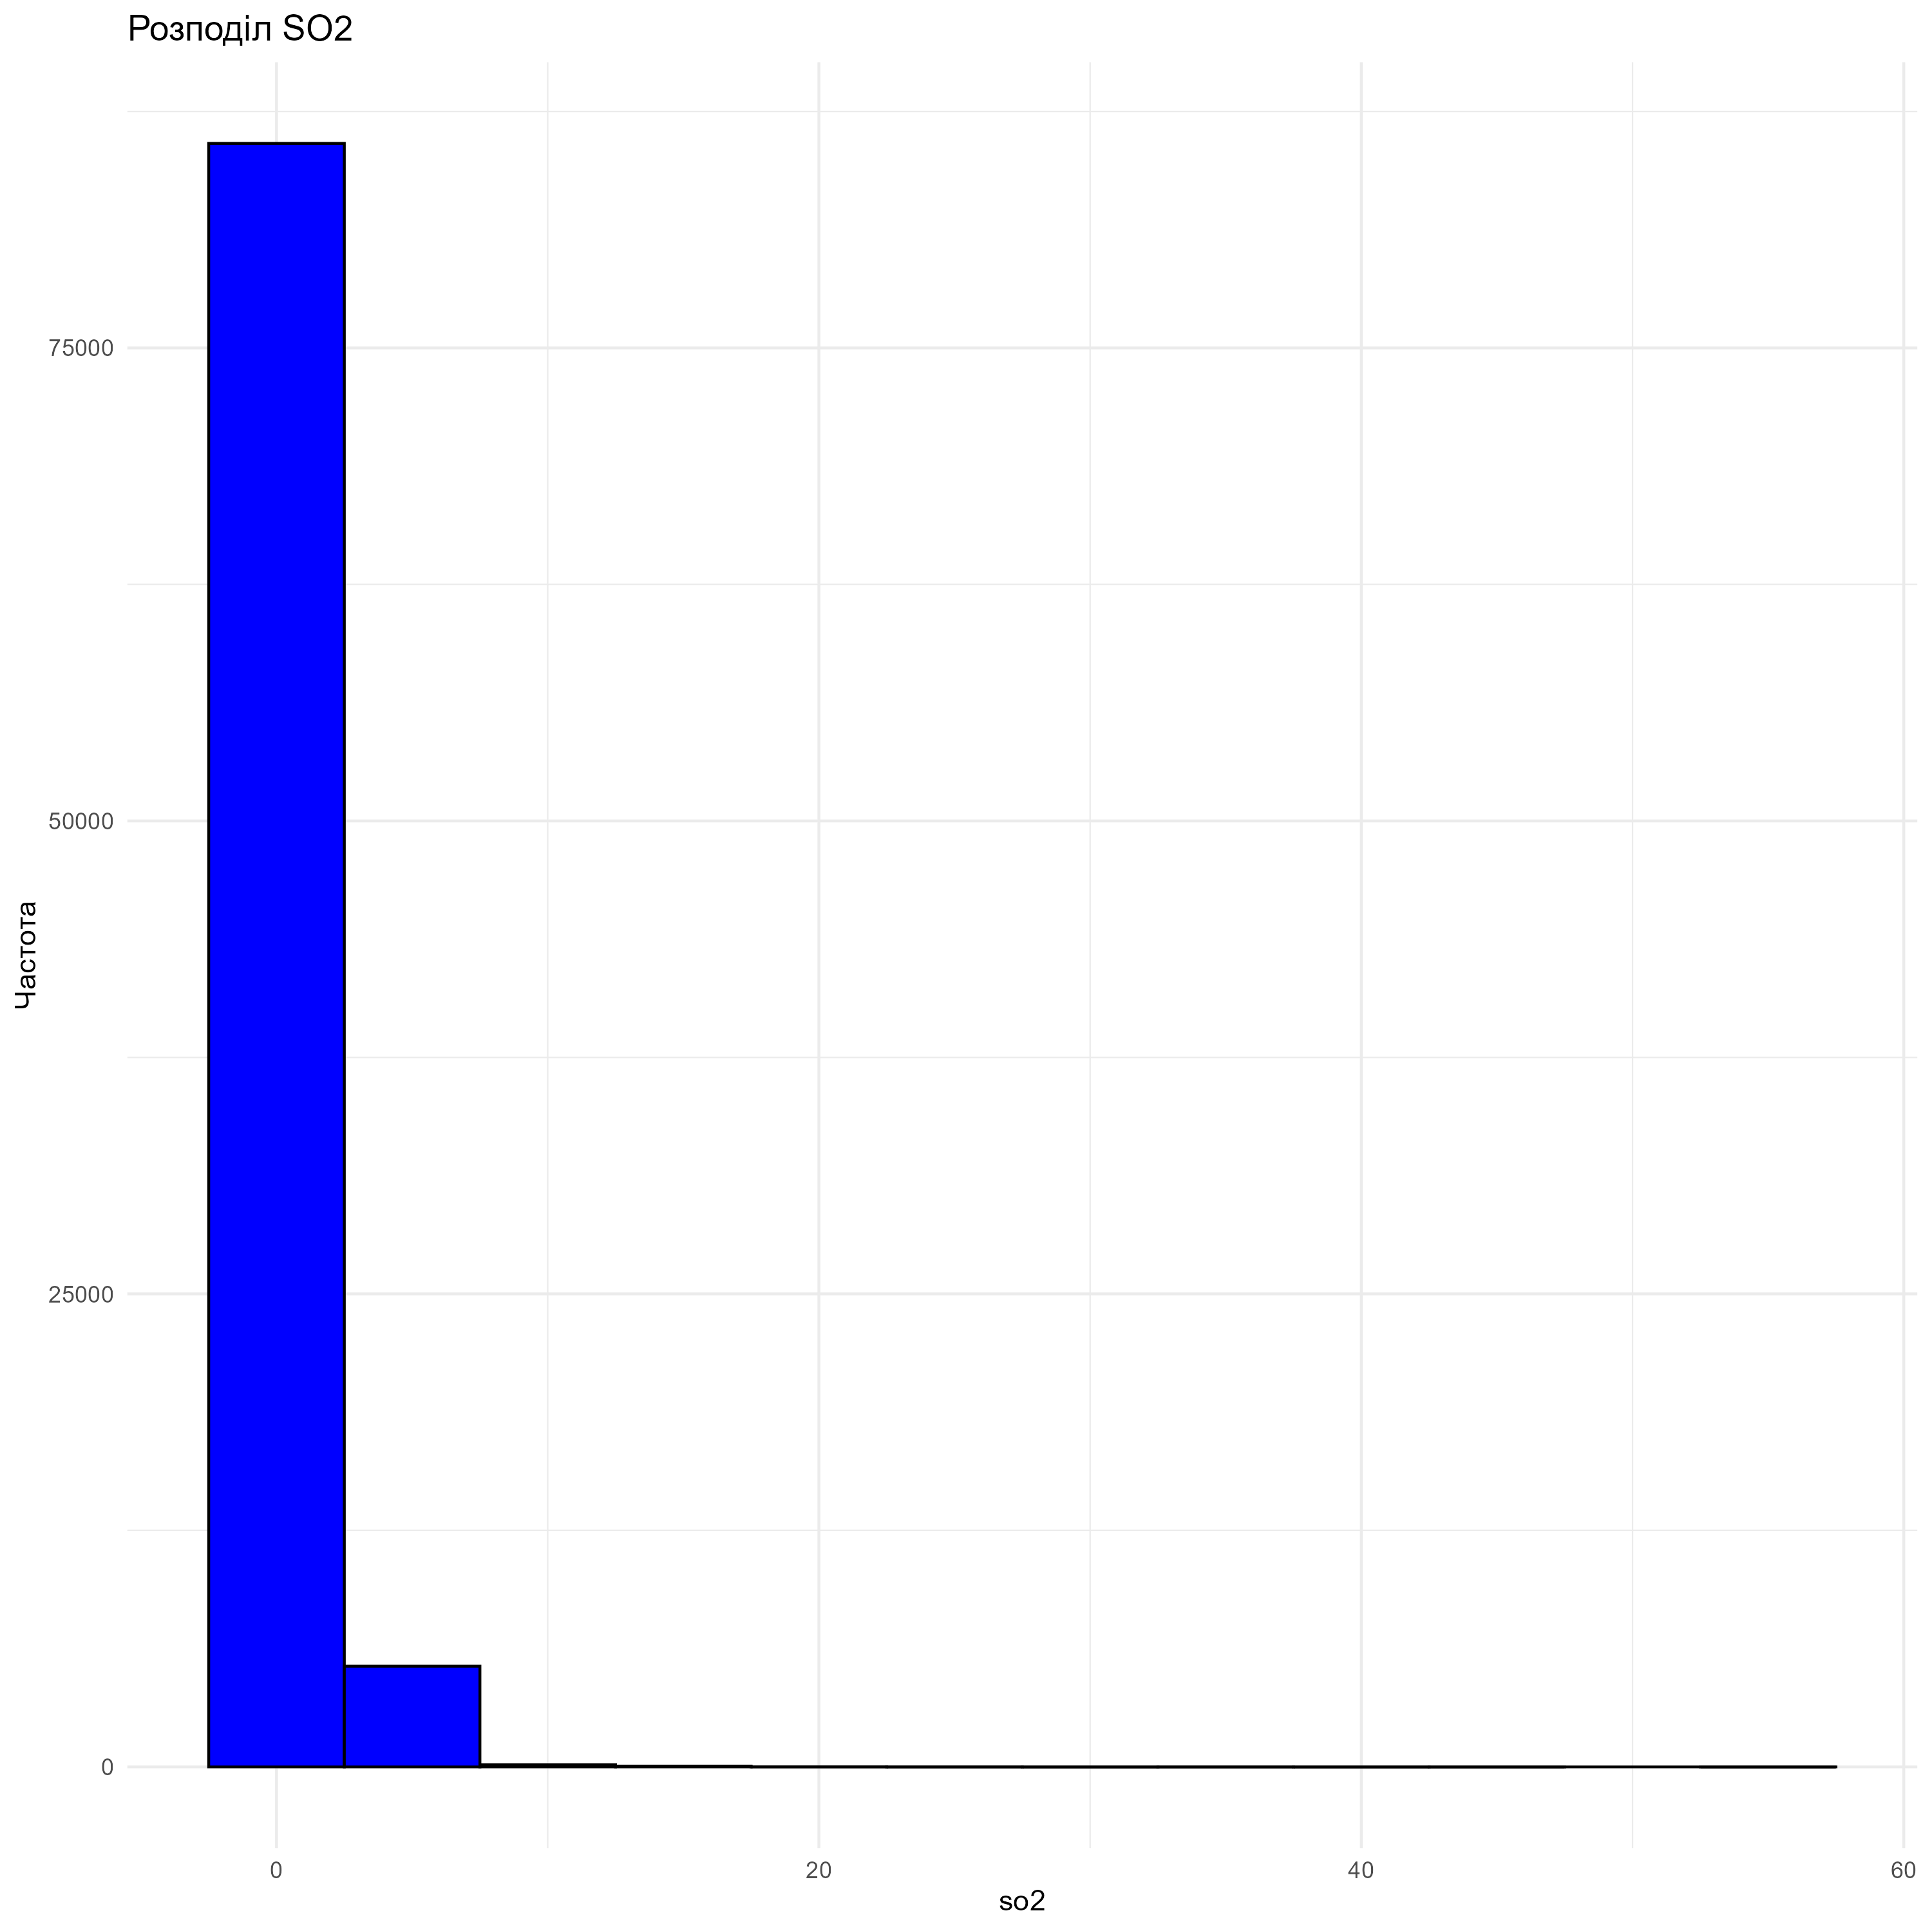
\includegraphics[height=2.8in]{plots/question2/so2_plot.png}
  \end{center}
\end{frame}

\begin{frame}
  \frametitle{Як зміни в концентрації $O_3$ та $SO_2$ впливають на загальний рівень забруднення повітря (AQI)?}

  \begin{center}
    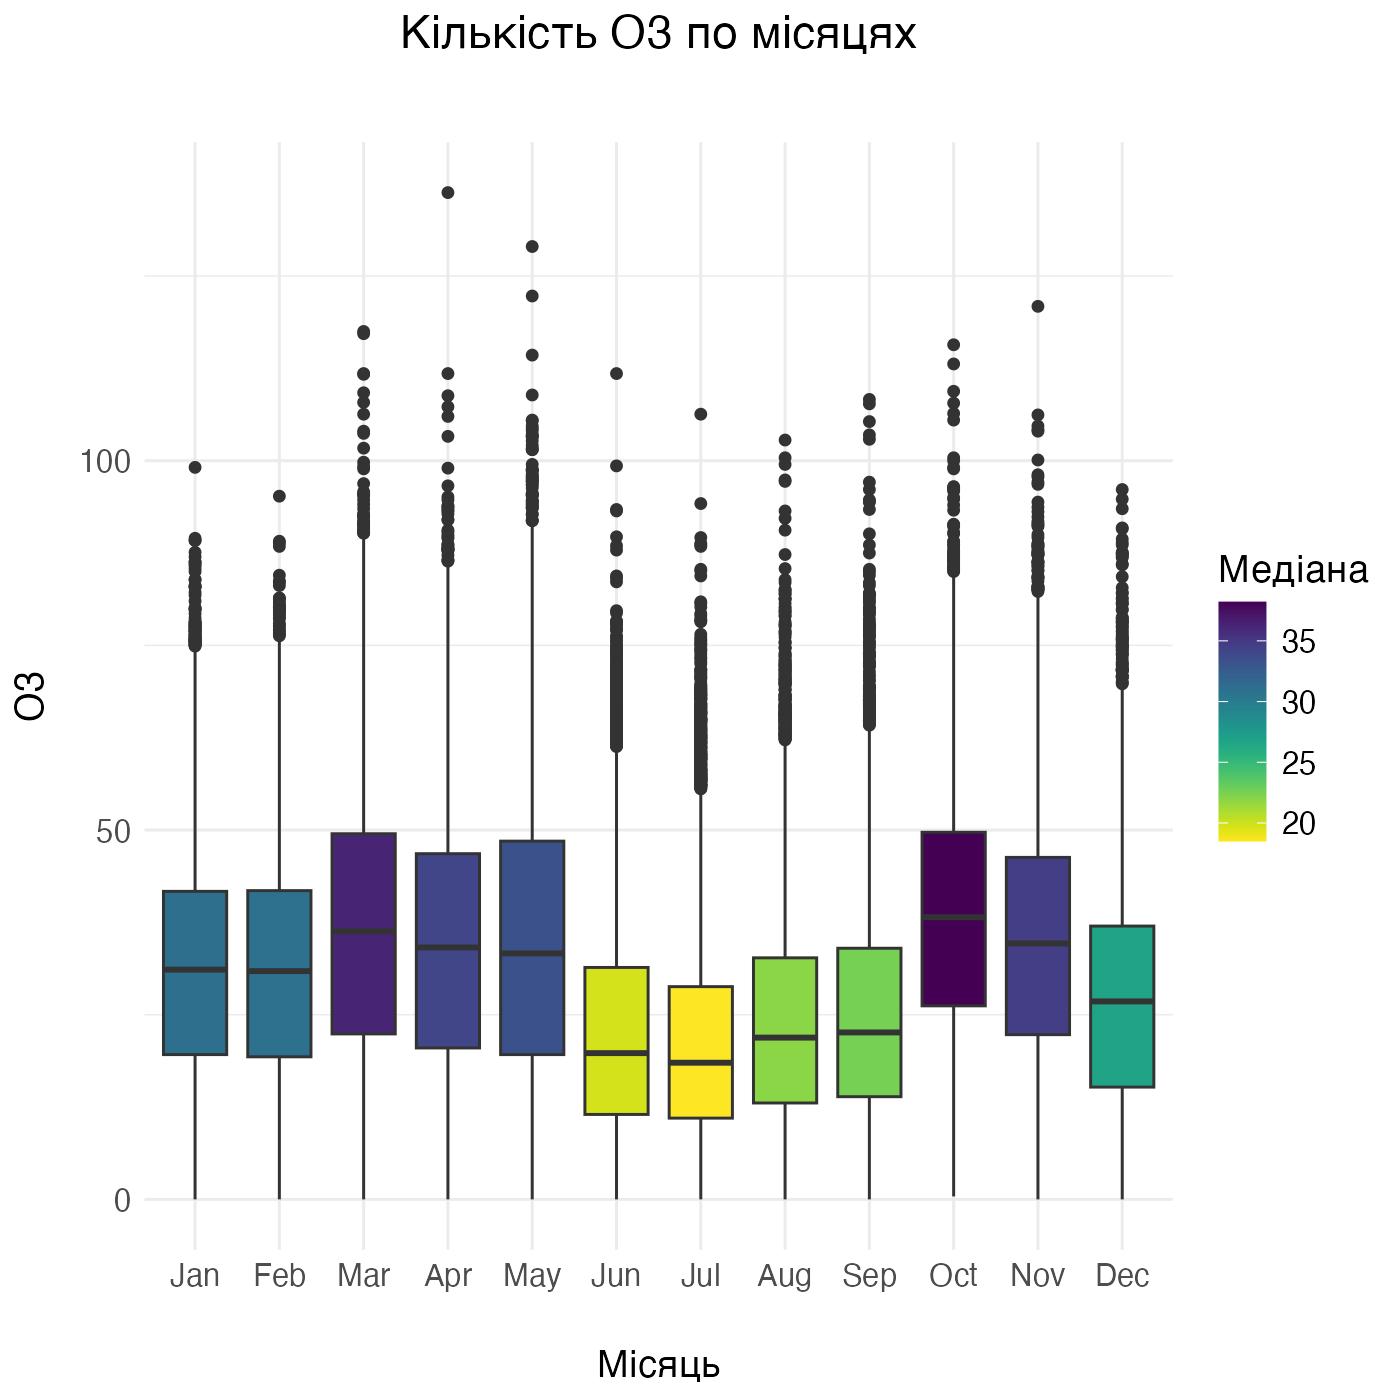
\includegraphics[height=2.8in]{plots/question2/seasonal_o3.png}
  \end{center}
\end{frame}

\begin{frame}
  \frametitle{Як зміни в концентрації $O_3$ та $SO_2$ впливають на загальний рівень забруднення повітря (AQI)?}

  \begin{center}
    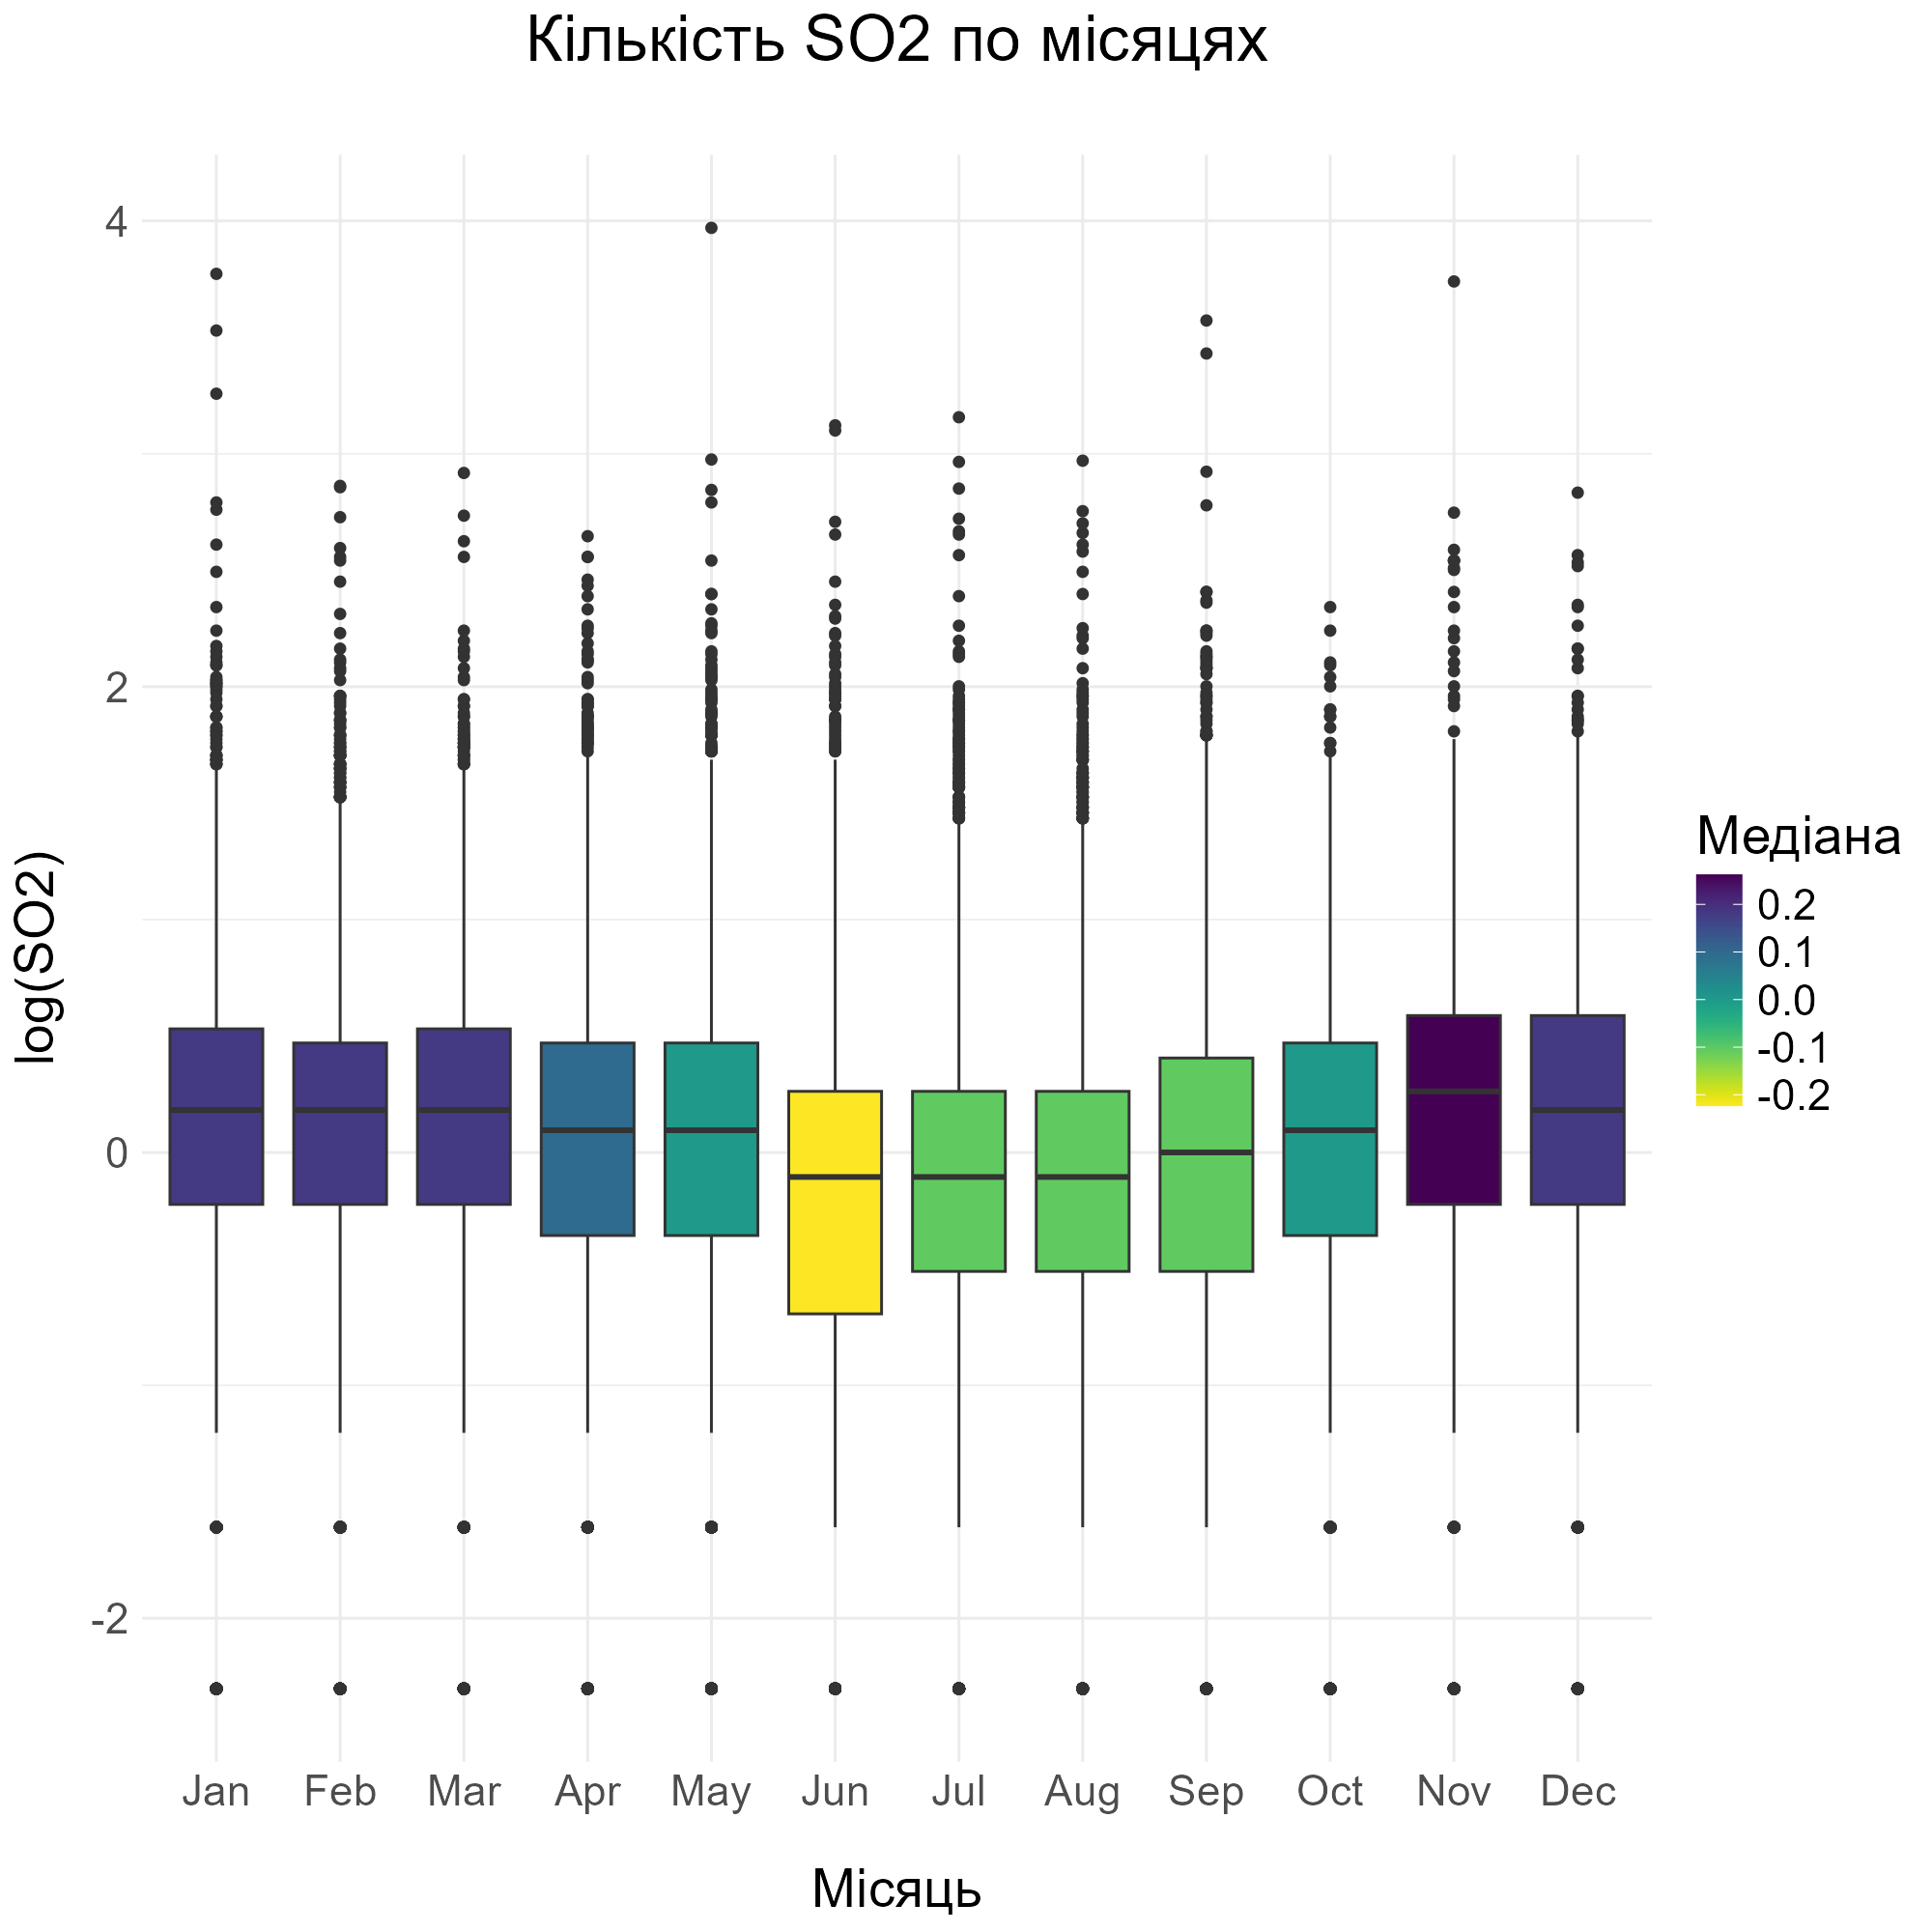
\includegraphics[height=2.8in]{plots/question2/seasonal_so2.png}
  \end{center}
\end{frame}

\begin{frame}
  \frametitle{Як зміни в концентрації $O_3$ та $SO_2$ впливають на загальний рівень забруднення повітря (AQI)?}

  \begin{center}
    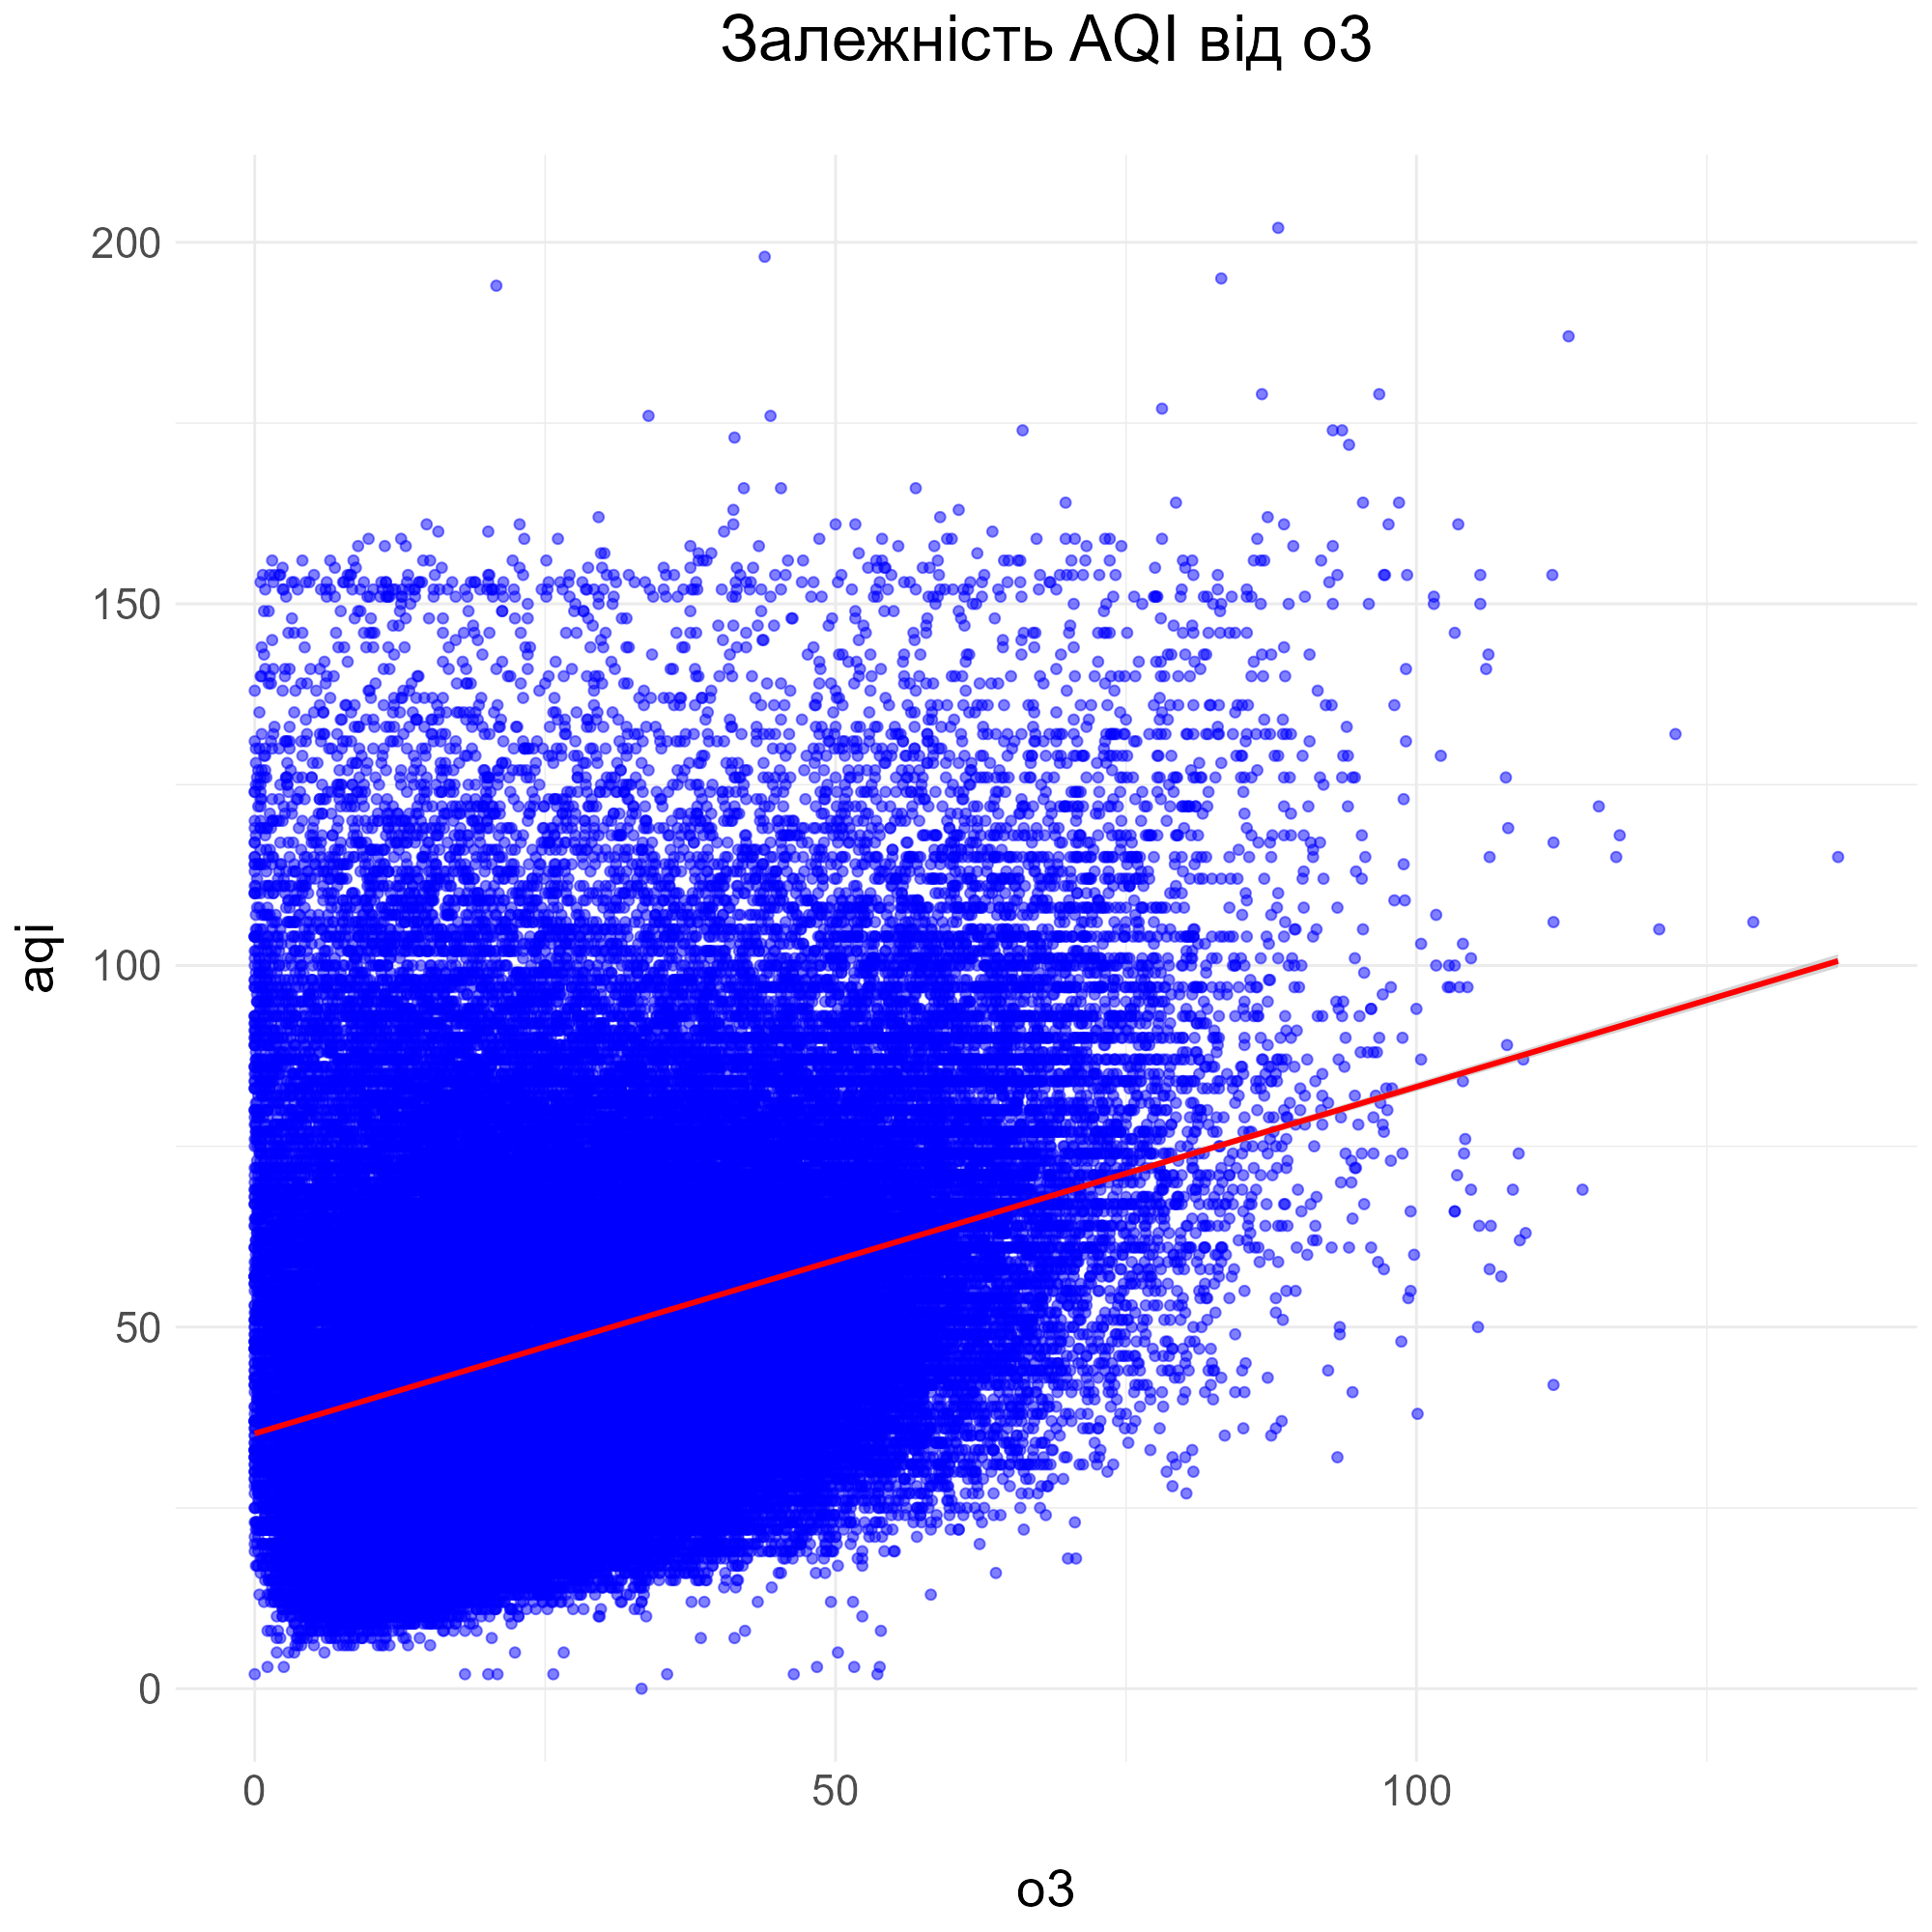
\includegraphics[height=2.8in]{plots/question2/scatter_plot_o3.png}
  \end{center}
\end{frame}

\begin{frame}
  \frametitle{Як зміни в концентрації $O_3$ та $SO_2$ впливають на загальний рівень забруднення повітря (AQI)?}

  \begin{center}
    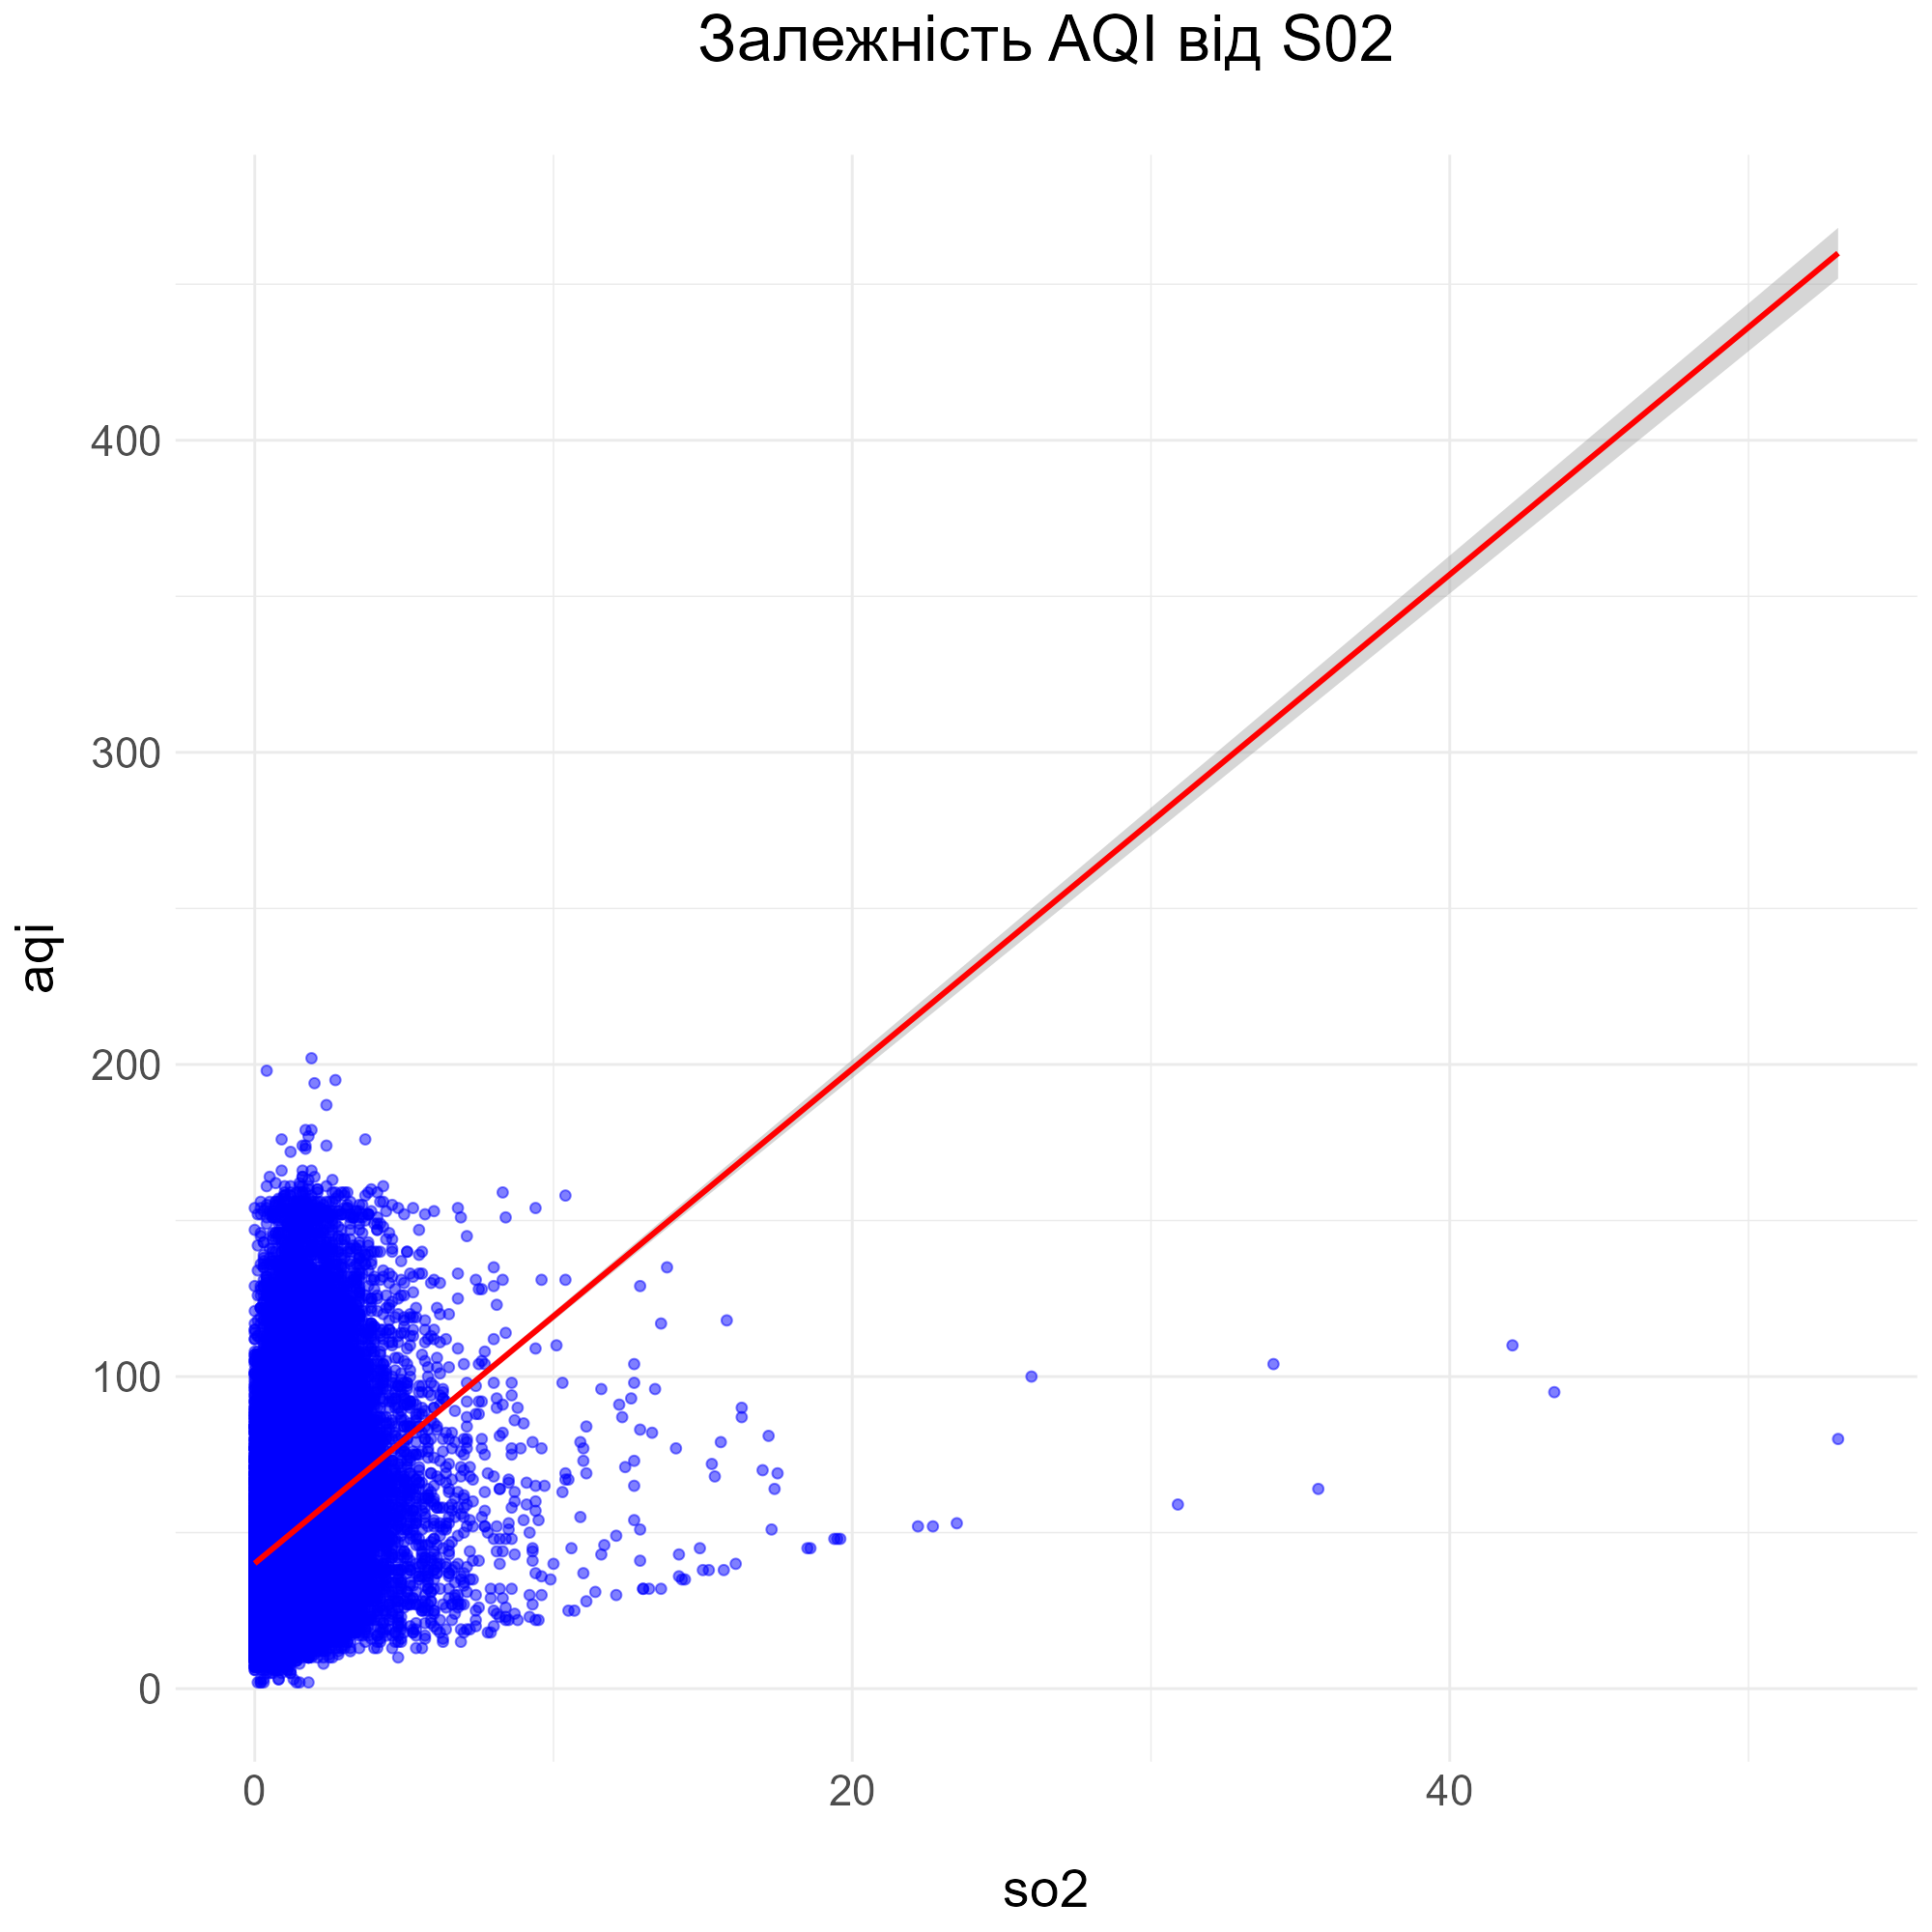
\includegraphics[height=2.8in]{plots/question2/scatter_plot_so2.png}
  \end{center}
\end{frame}

\begin{frame}
  \frametitle{Як зміни в концентрації $O_3$ та $SO_2$ впливають на загальний рівень забруднення повітря (AQI)?}

  \begin{enumerate}
    \item Спостерігається позитивна залежність між концентрацією $O_3$ та AQI: зростання озону супроводжується збільшенням індексу забруднення.
    \item Спостерігається підвищена концентрація $O_3$ та відповідно відносно не значна $SO_2$.
  \end{enumerate}
\end{frame}

%% Question 3

\begin{frame}
  \frametitle{Як змінюється якість повітря протягом доби в різних районах?}

  \begin{center}
    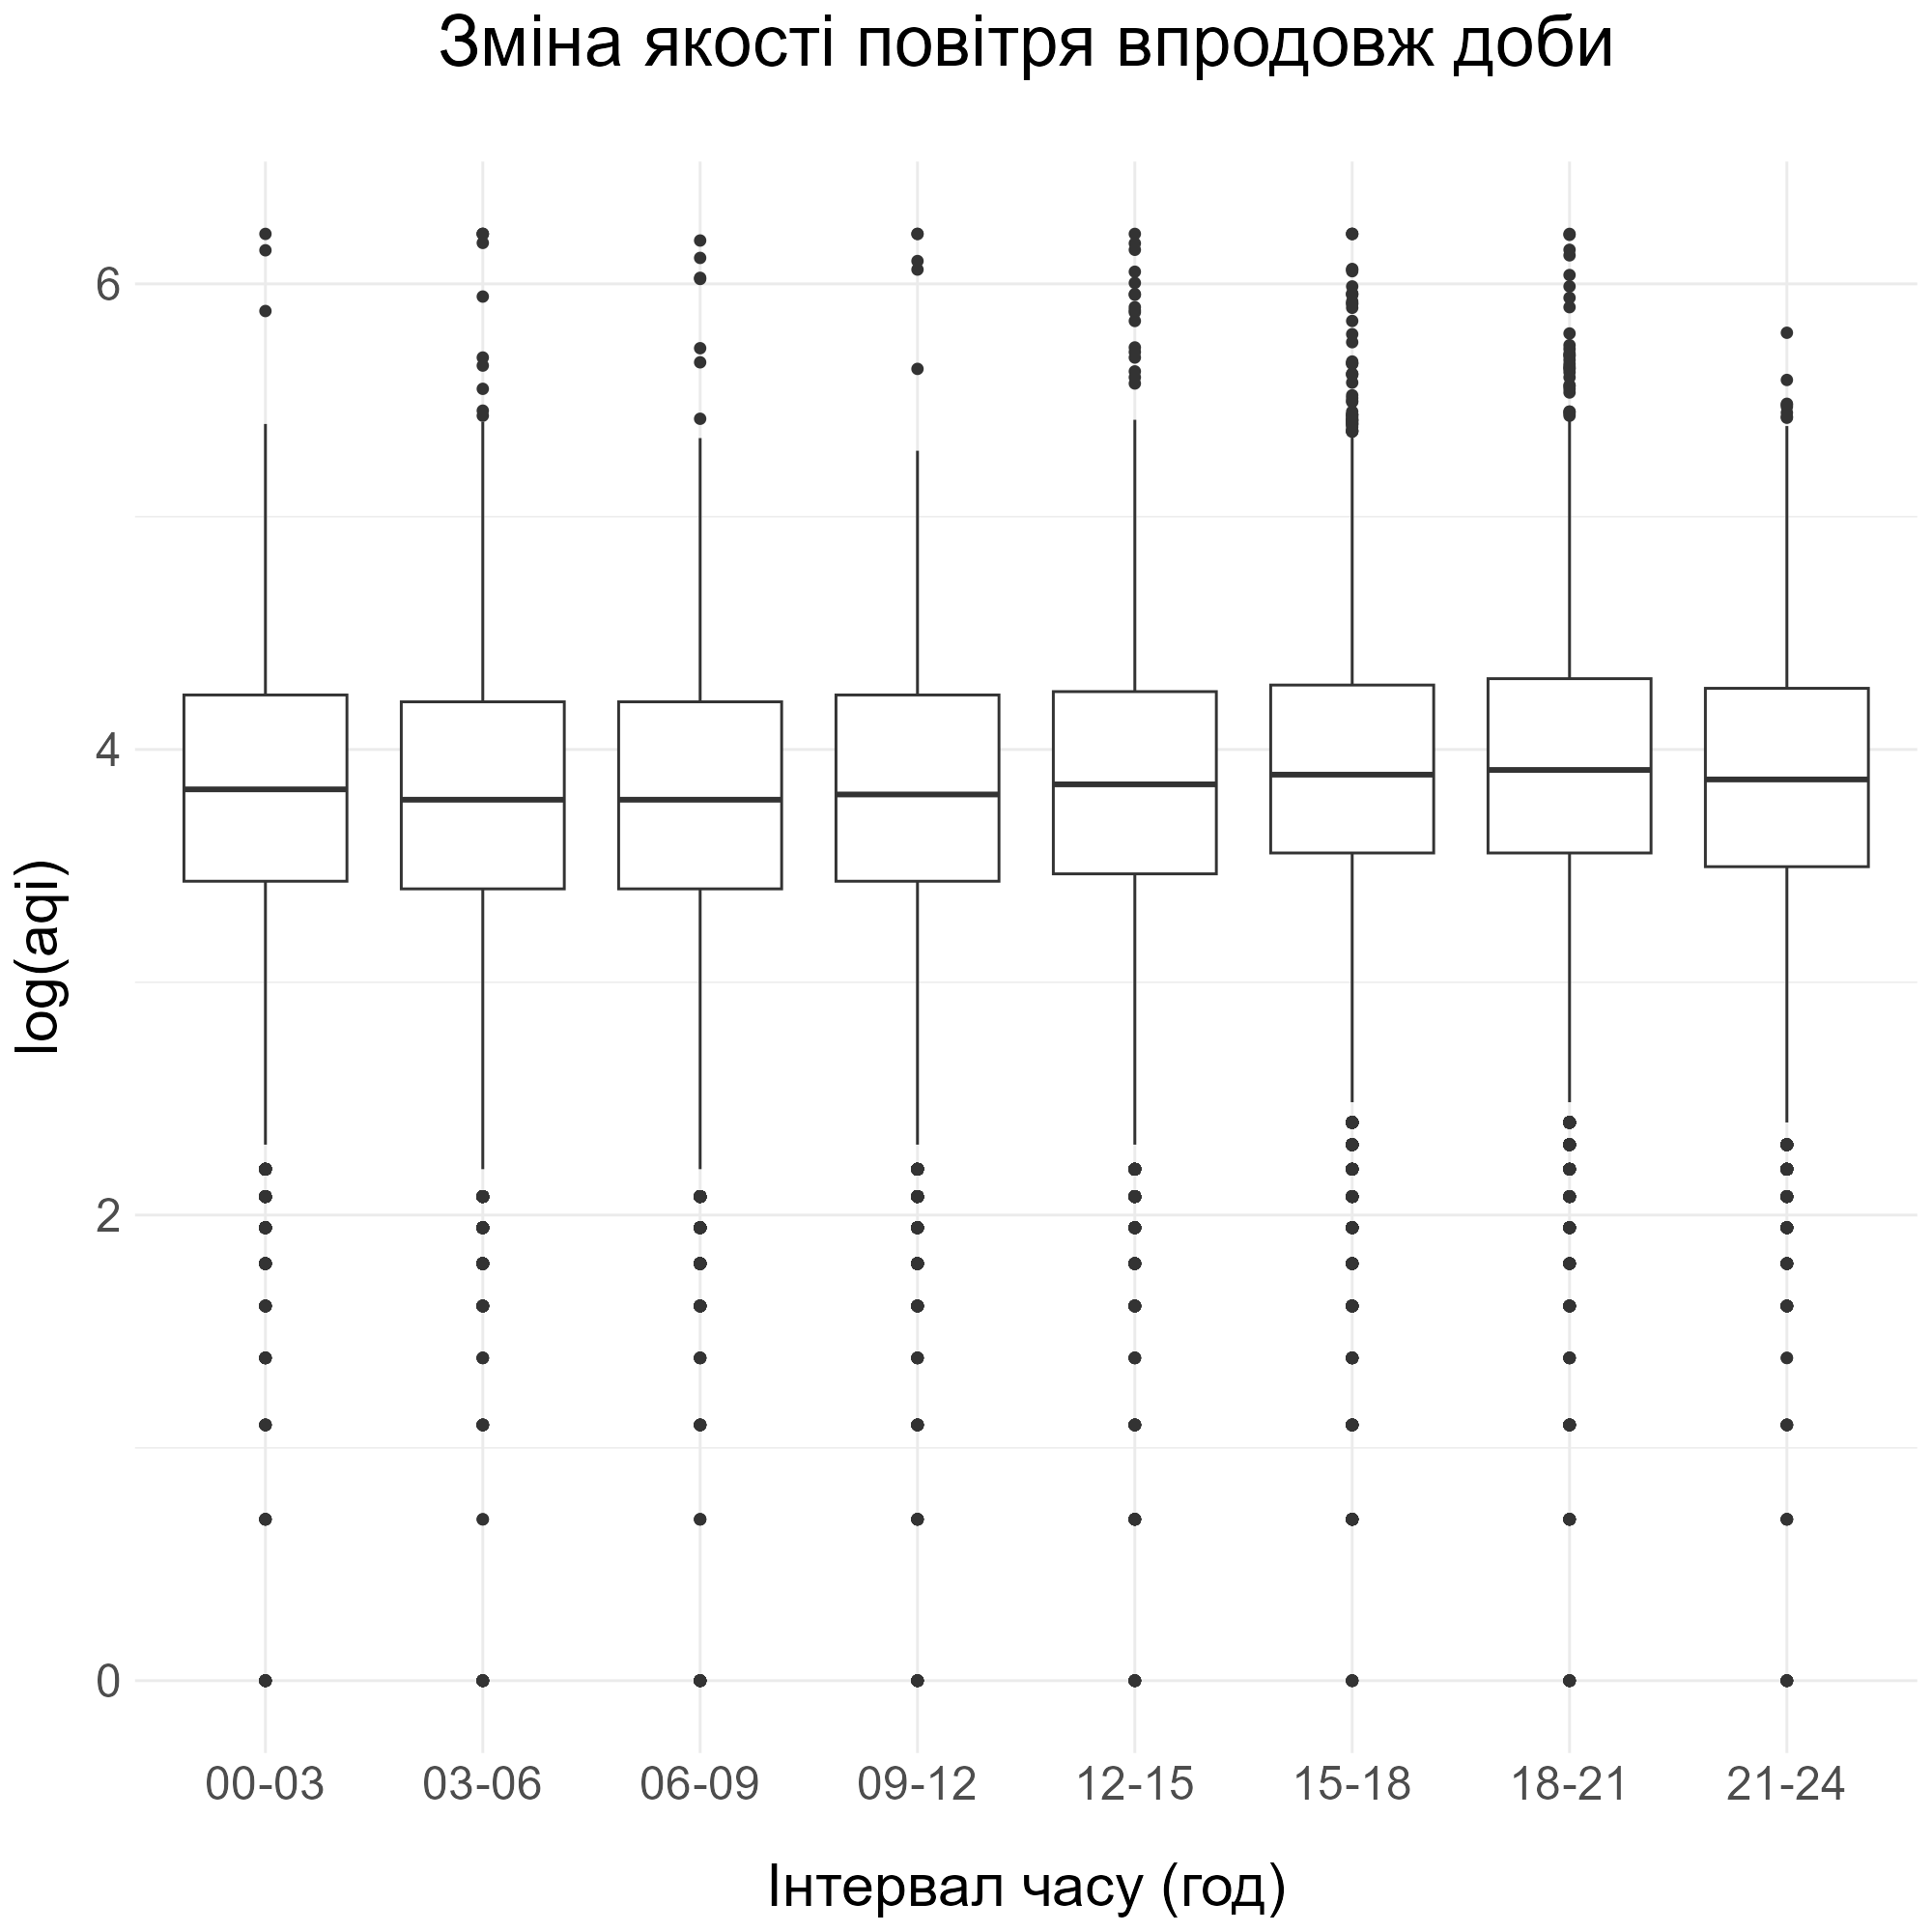
\includegraphics[height=2.8in]{plots/question3/box.png}
  \end{center}
\end{frame}

\begin{frame}
  \frametitle{Як змінюється якість повітря протягом доби в різних районах?}

  \begin{enumerate}
    \item Аналізуючи даний графік, можна стверджувати, що якість повітря трохи
    погіршується у другій половині дня.
    \item Те ж спостерігається і по окремих районах.
  \end{enumerate}
\end{frame}

\begin{frame}
  \frametitle{Як змінюється якість повітря протягом доби в різних районах?}

  \begin{center}
    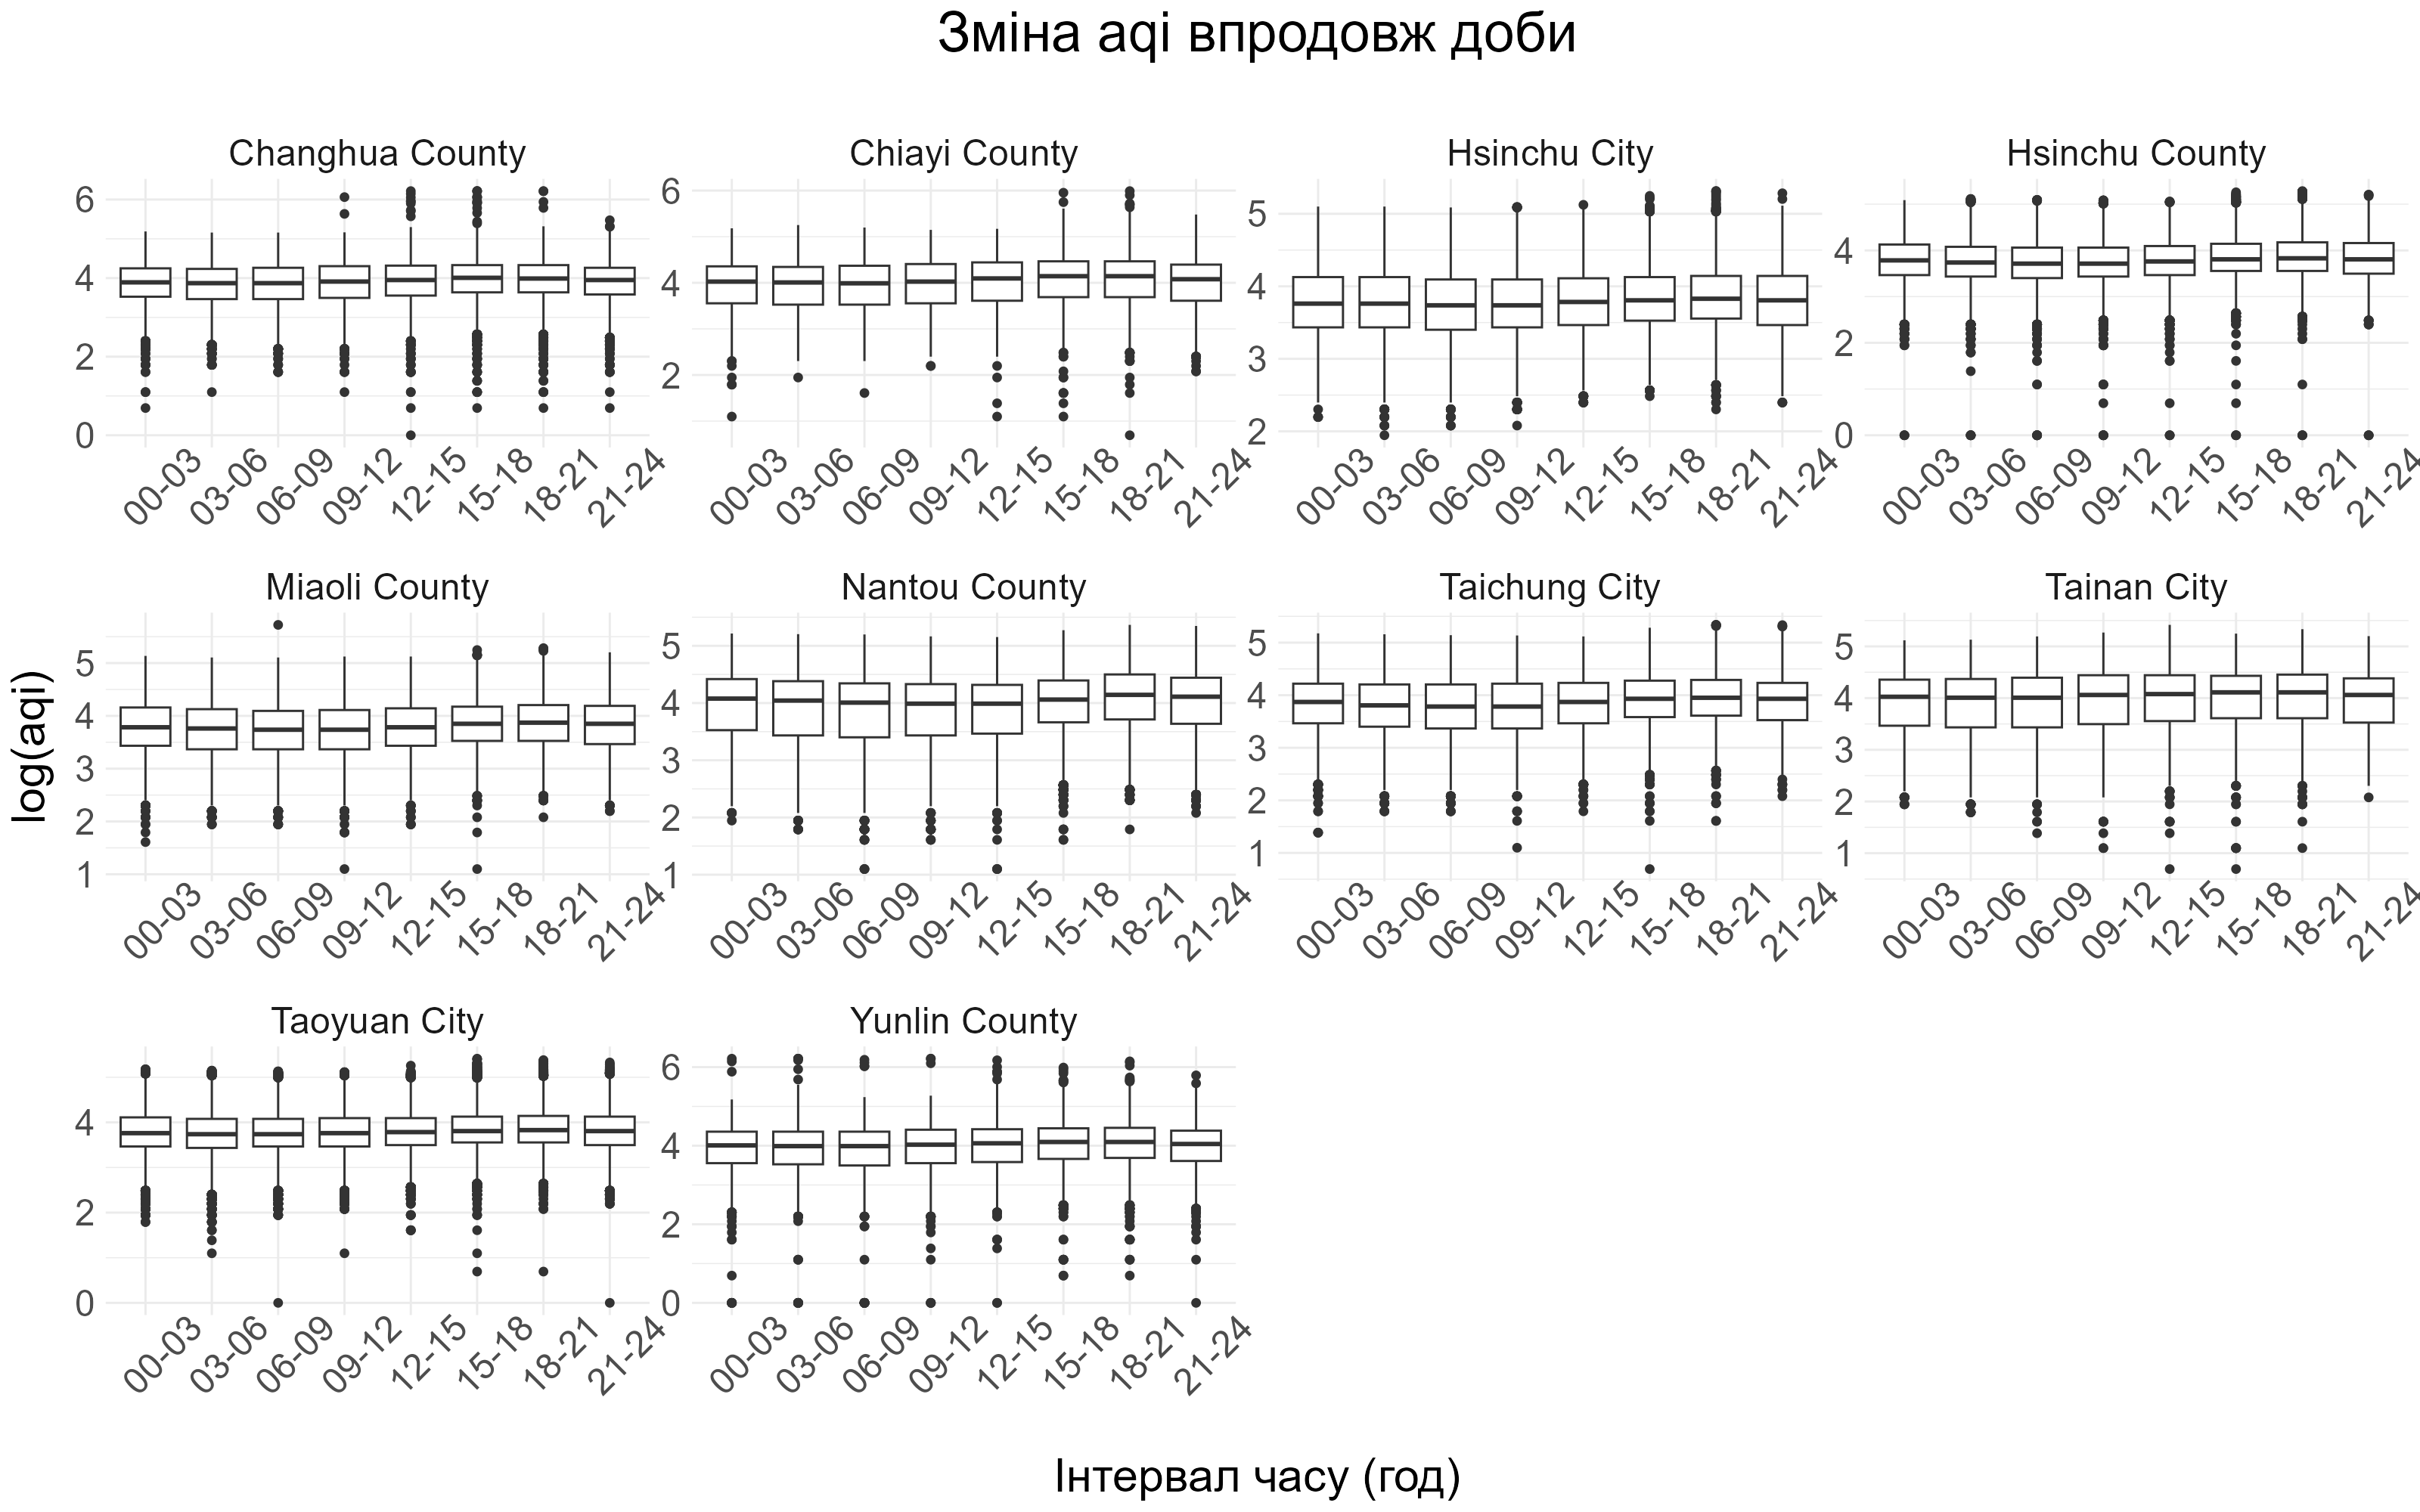
\includegraphics[height=2.8in]{plots/question3/county-box-p1.png}
  \end{center}
\end{frame}

\begin{frame}
  \frametitle{Як змінюється якість повітря протягом доби в різних районах?}

  \begin{center}
    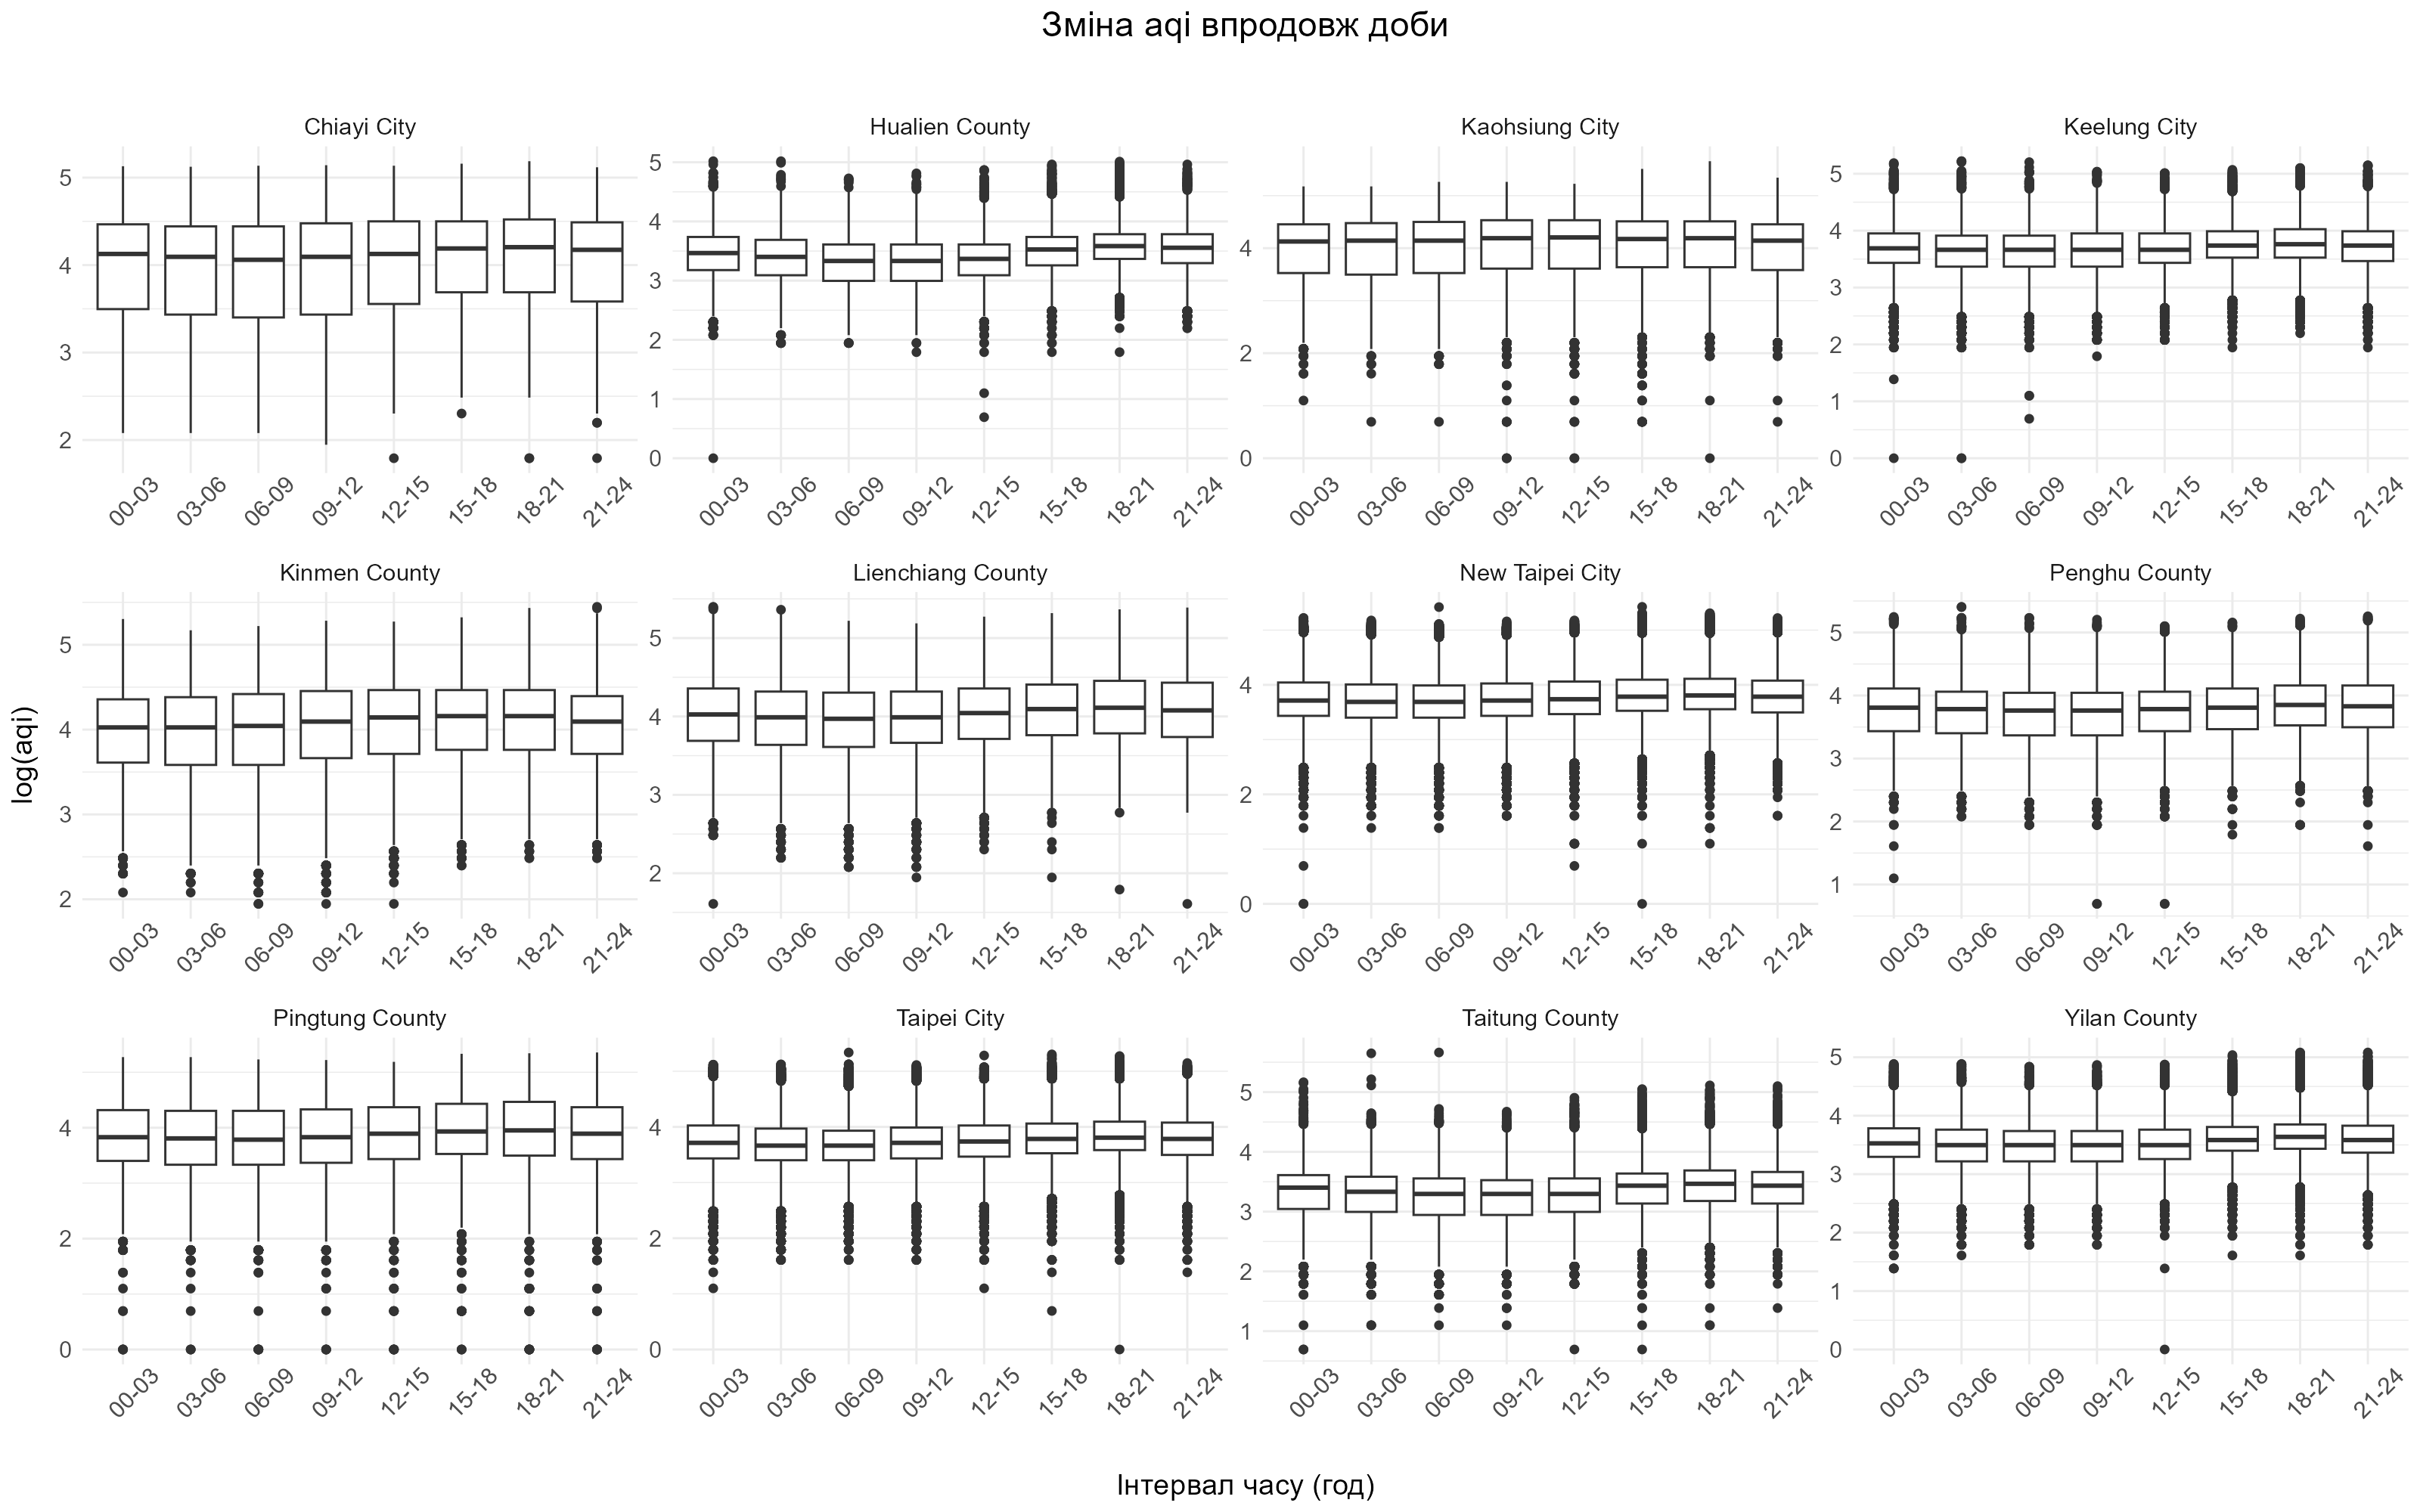
\includegraphics[height=2.8in]{plots/question3/county-box-p2.png}
  \end{center}
\end{frame}

\begin{frame}
  \frametitle{Як змінюється якість повітря протягом доби в різних районах?}

  \begin{enumerate}
    \item Бачимо, що зміни впродовж дня є, проте вони не суттєві.
  \end{enumerate}
\end{frame}

%% Question 4

\begin{frame}
  \frametitle{Які регіони мають найвищий середній рівень забруднення повітря (AQI) протягом року?}

  \textit{Був використаний trimmed набір даних}

  \begin{enumerate}
    \item Всі наступні графіки, будуть будуватися на основі даних за
    2016, 2017, 2023 та 2024 роки.
    \item  Для розуміння числових даних, розглянемо 10 регіонів з
    найвищим рівнем AQI за відповідні роки.
  \end{enumerate}
\end{frame}

\begin{frame}
  \frametitle{Які регіони мають найвищий середній рівень забруднення повітря (AQI) протягом року?}

  \begin{center}
    \begin{tabular}{clc}
      \textbf{Year} & \textbf{Сounty} & \textbf{Average AQI} \\
      2016 & Chiayi City     & 120.31 \\
      2016 & Kaohsiung City  & 112.10 \\
      2016 & Tainan City     & 99.60  \\
      2016 & Pingtung County & 97.15  \\
      2016 & Yunlin County   & 91.23  \\
      2016 & Chiayi County   & 88.83  \\
      2016 & Nantou County   & 83.34  \\
      2016 & Changhua County & 81.68  \\
      2016 & Kinmen County   & 81.60  \\
      2016 & Taichung City   & 77.96  \\
    \end{tabular}
  \end{center}
\end{frame}

\begin{frame}
  \frametitle{Які регіони мають найвищий середній рівень забруднення повітря (AQI) протягом року?}

  \begin{center}
    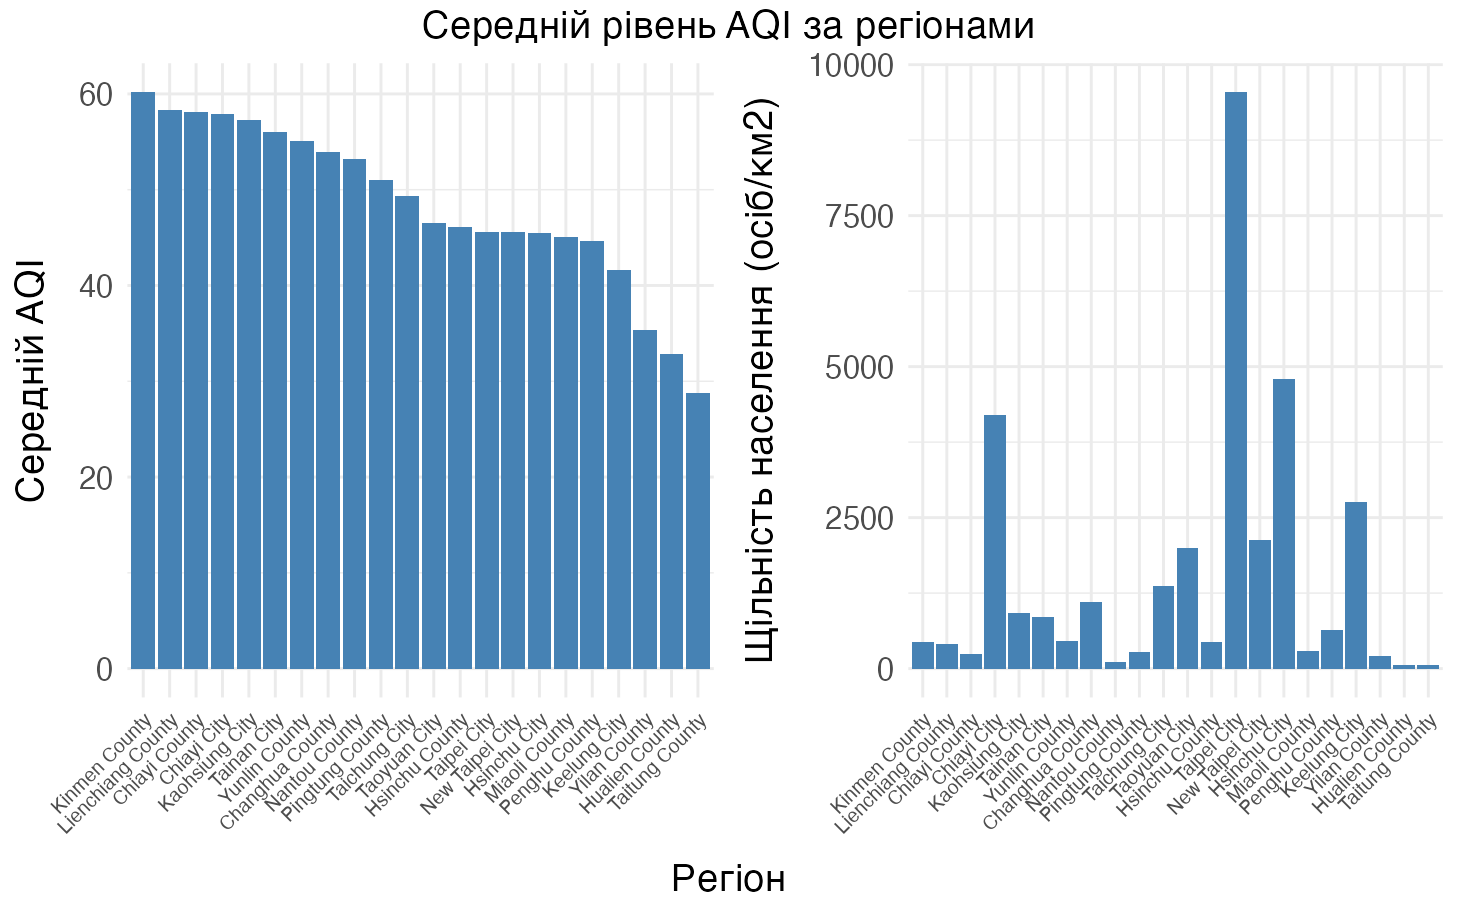
\includegraphics[height=2.8in]{plots/question4/avg_aqi_by_county_w_dens.png}
  \end{center}
\end{frame}

\begin{frame}
  \frametitle{Які регіони мають найвищий середній рівень забруднення повітря (AQI) протягом року?}

  \begin{center}
    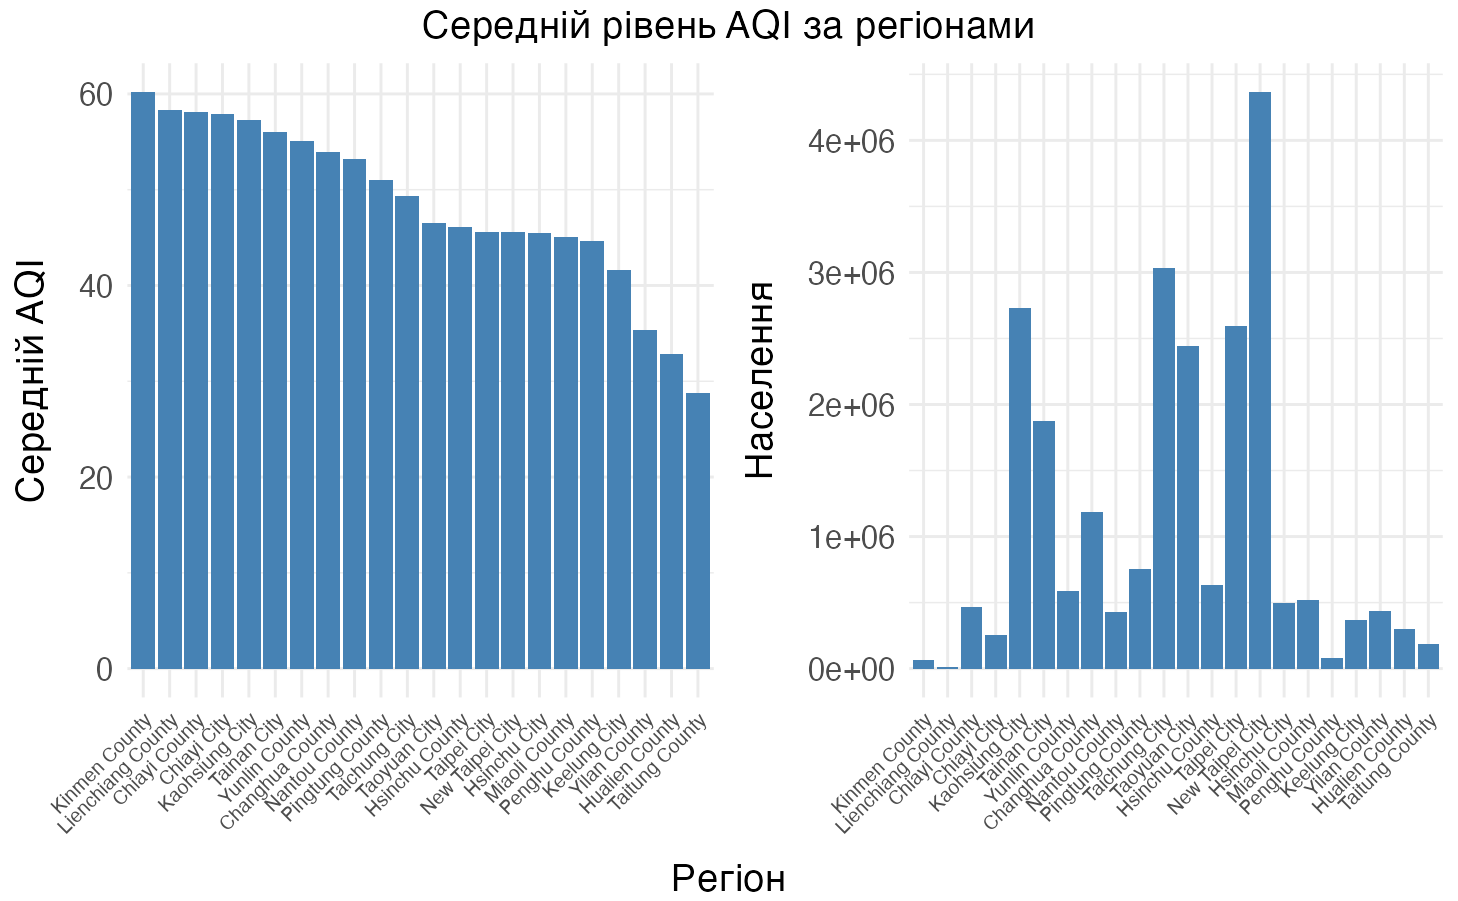
\includegraphics[height=2.8in]{plots/question4/avg_aqi_by_county_w_pop.png}
  \end{center}
\end{frame}

\begin{frame}
  \frametitle{Які регіони мають найвищий середній рівень забруднення повітря (AQI) протягом року?}

  \begin{center}
    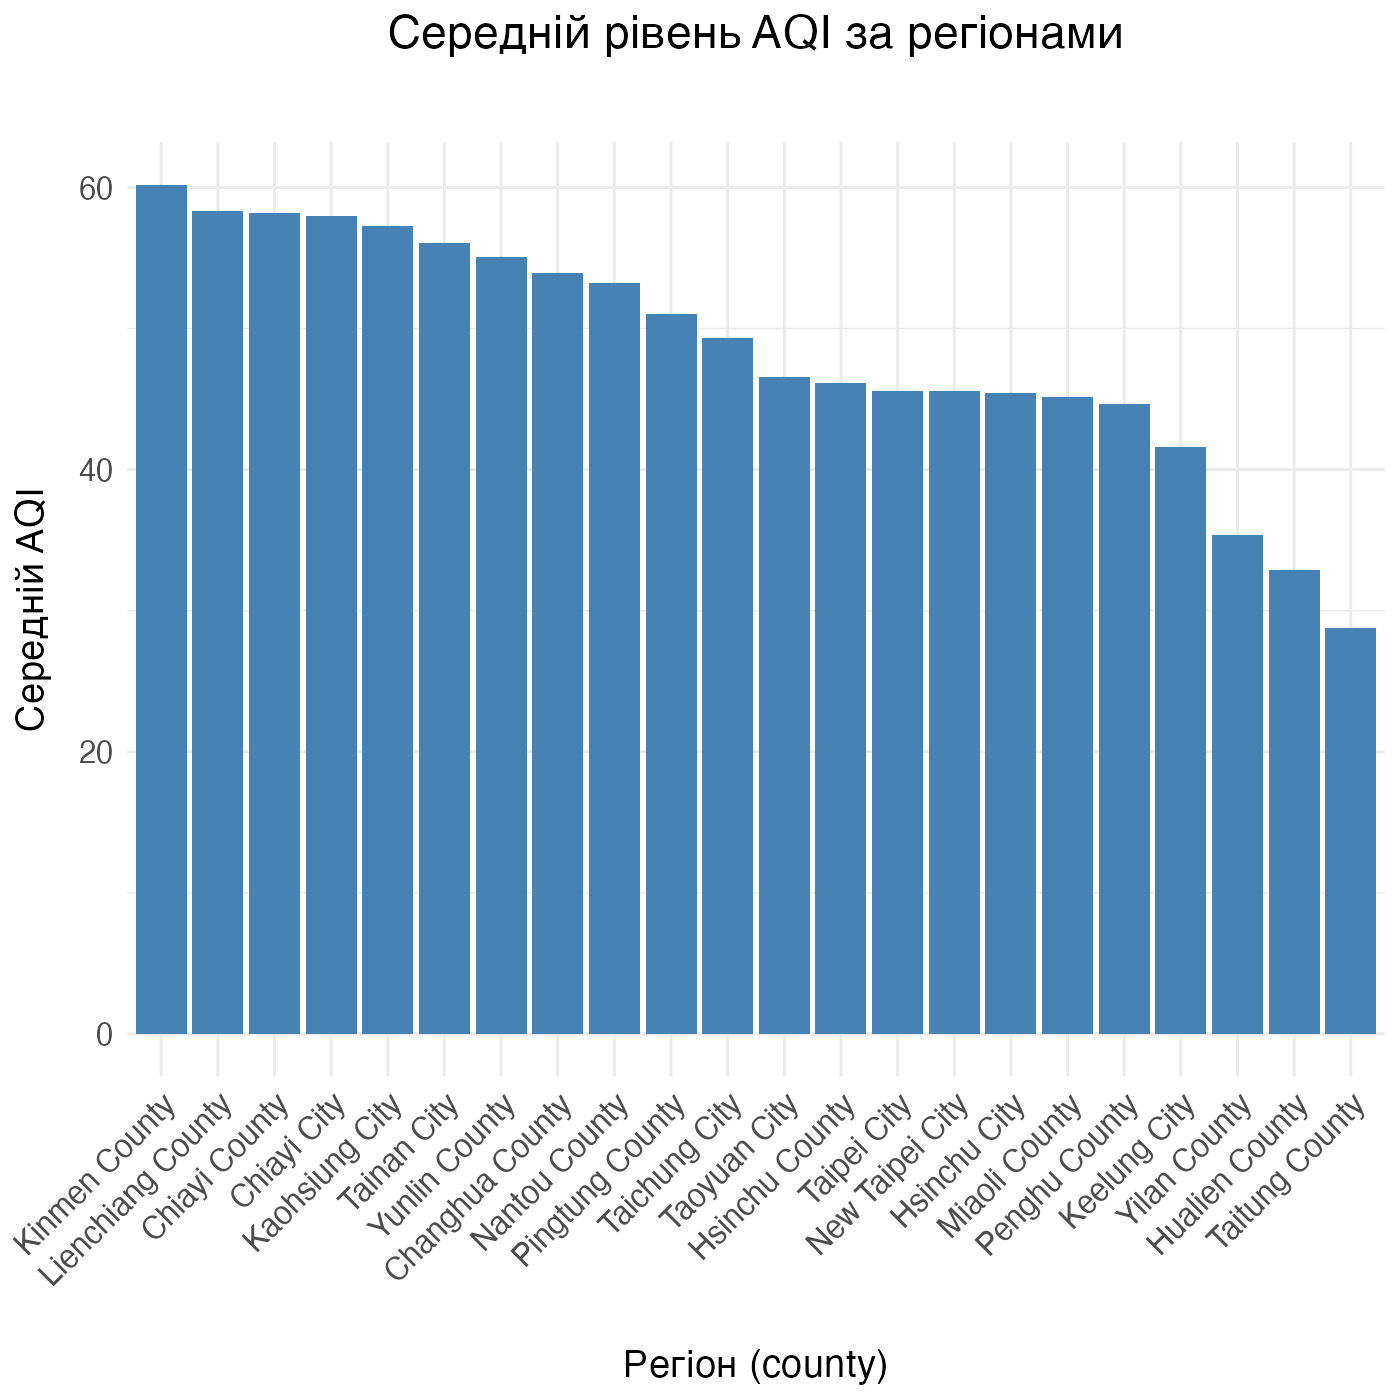
\includegraphics[height=2.8in]{plots/question4/avg_aqi_by_county.png}
  \end{center}
\end{frame}

\begin{frame}
  \frametitle{Які регіони мають найвищий середній рівень забруднення повітря (AQI) протягом року?}

  \begin{center}
    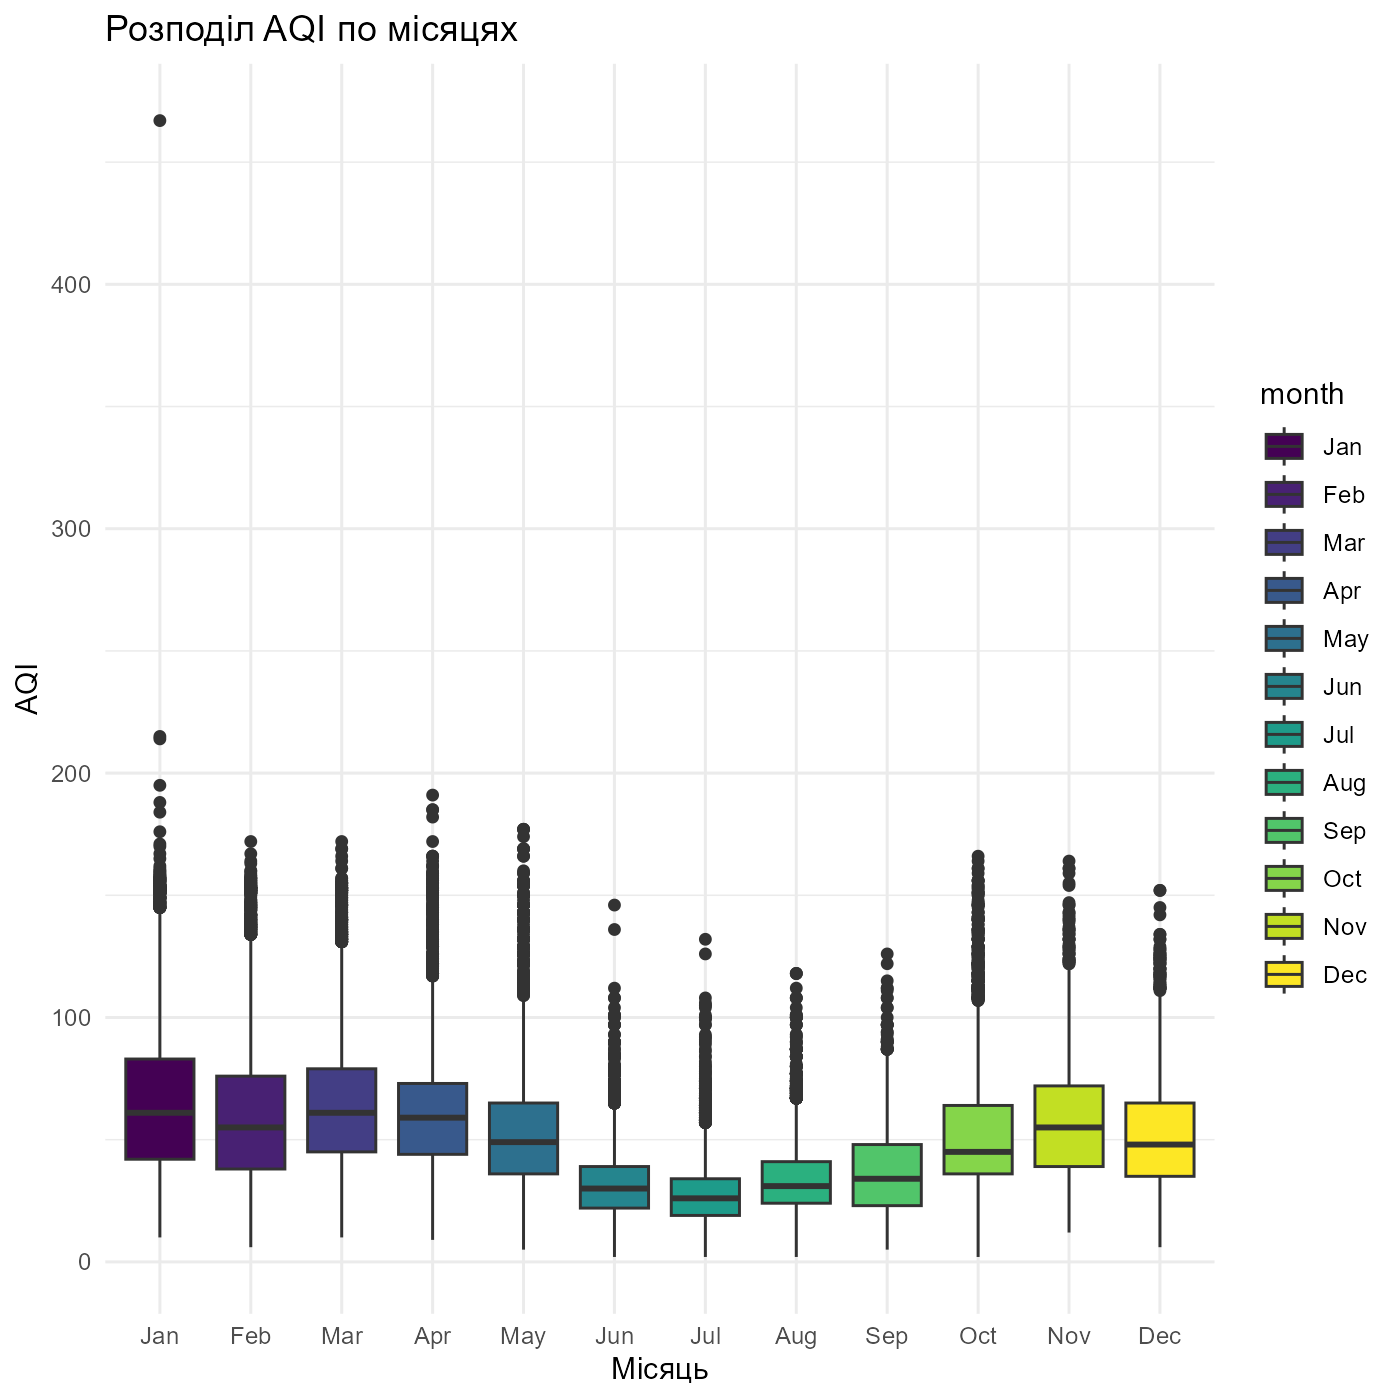
\includegraphics[height=2.8in]{plots/question4/seasonal_change.png}
  \end{center}
\end{frame}

\begin{frame}
  \frametitle{Які регіони мають найвищий середній рівень забруднення повітря (AQI) протягом року?}

  \begin{center}
    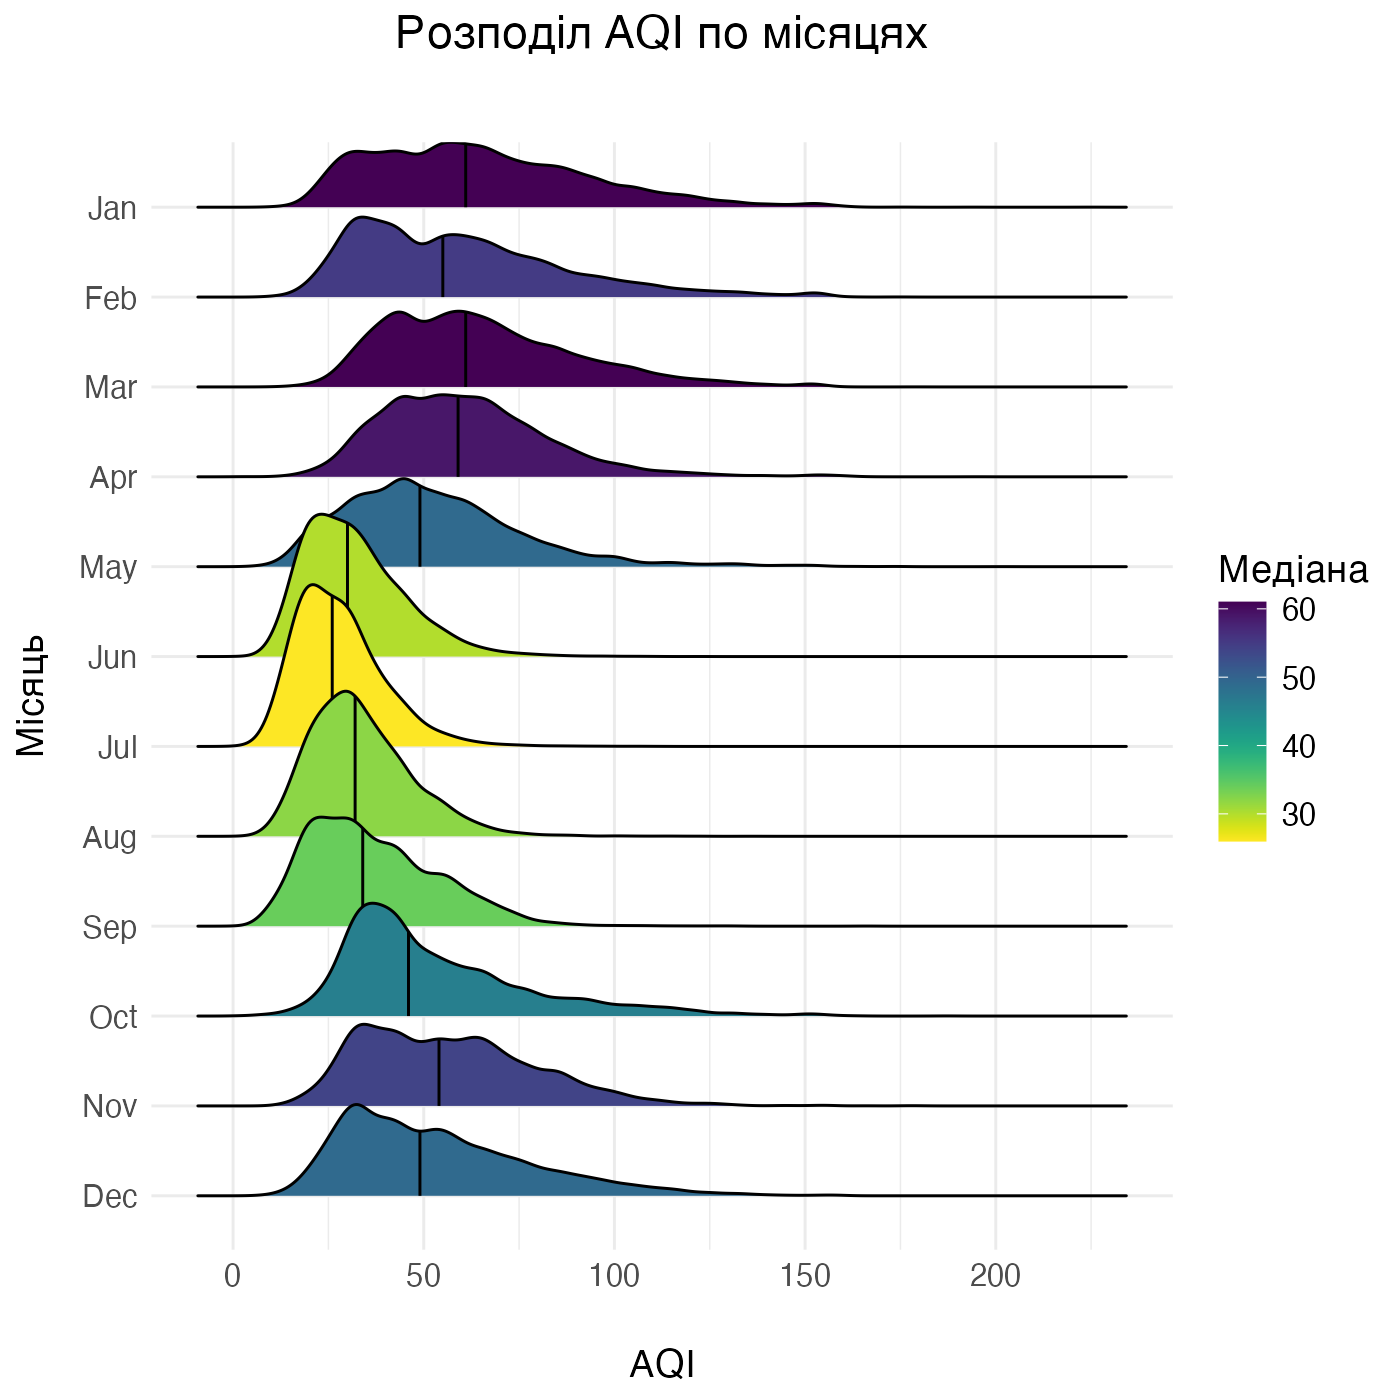
\includegraphics[height=2.8in]{plots/question4/seasonal_change_ridgeline.png}
  \end{center}
\end{frame}

%% Question 5

\begin{frame}
  \frametitle{Як змінився загальний рівень забруднення по регіонам після початку реформи?}

  \textit{Був використаний tidy набір даних}

  \begin{center}
    \begin{tabular}{cc}
      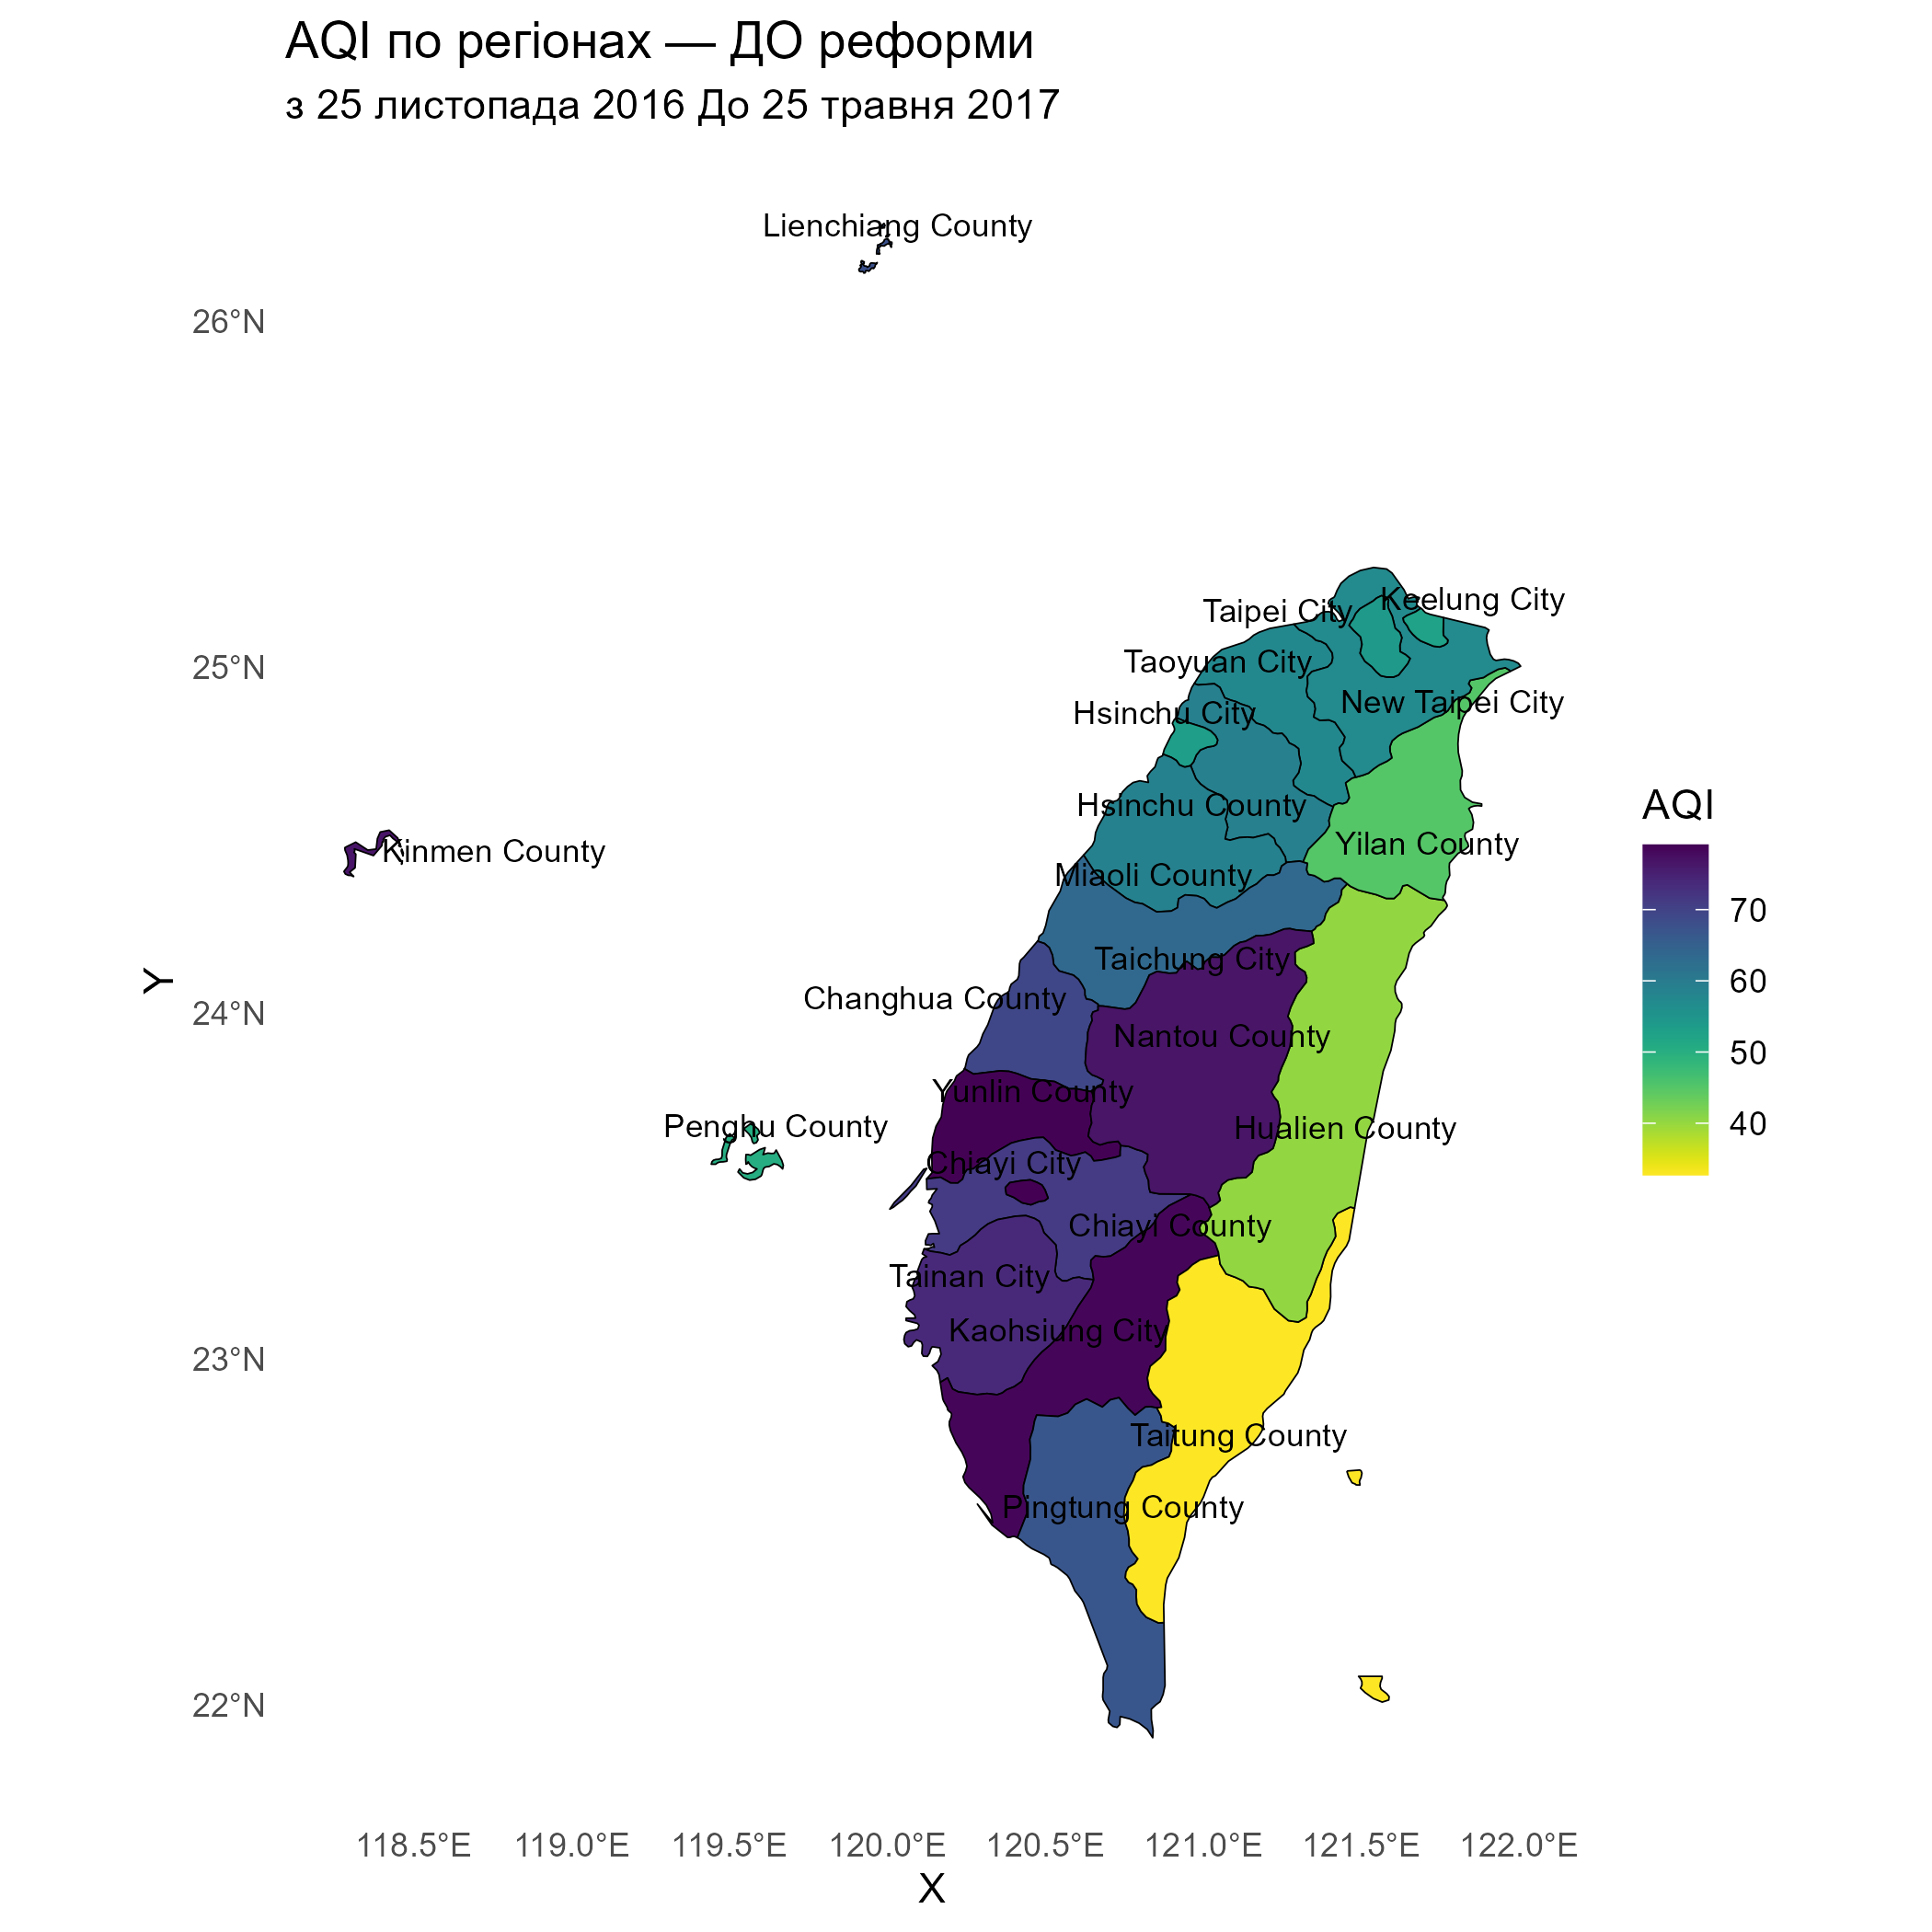
\includegraphics[height=2in]{plots/question5/map_before_reform.png} &
      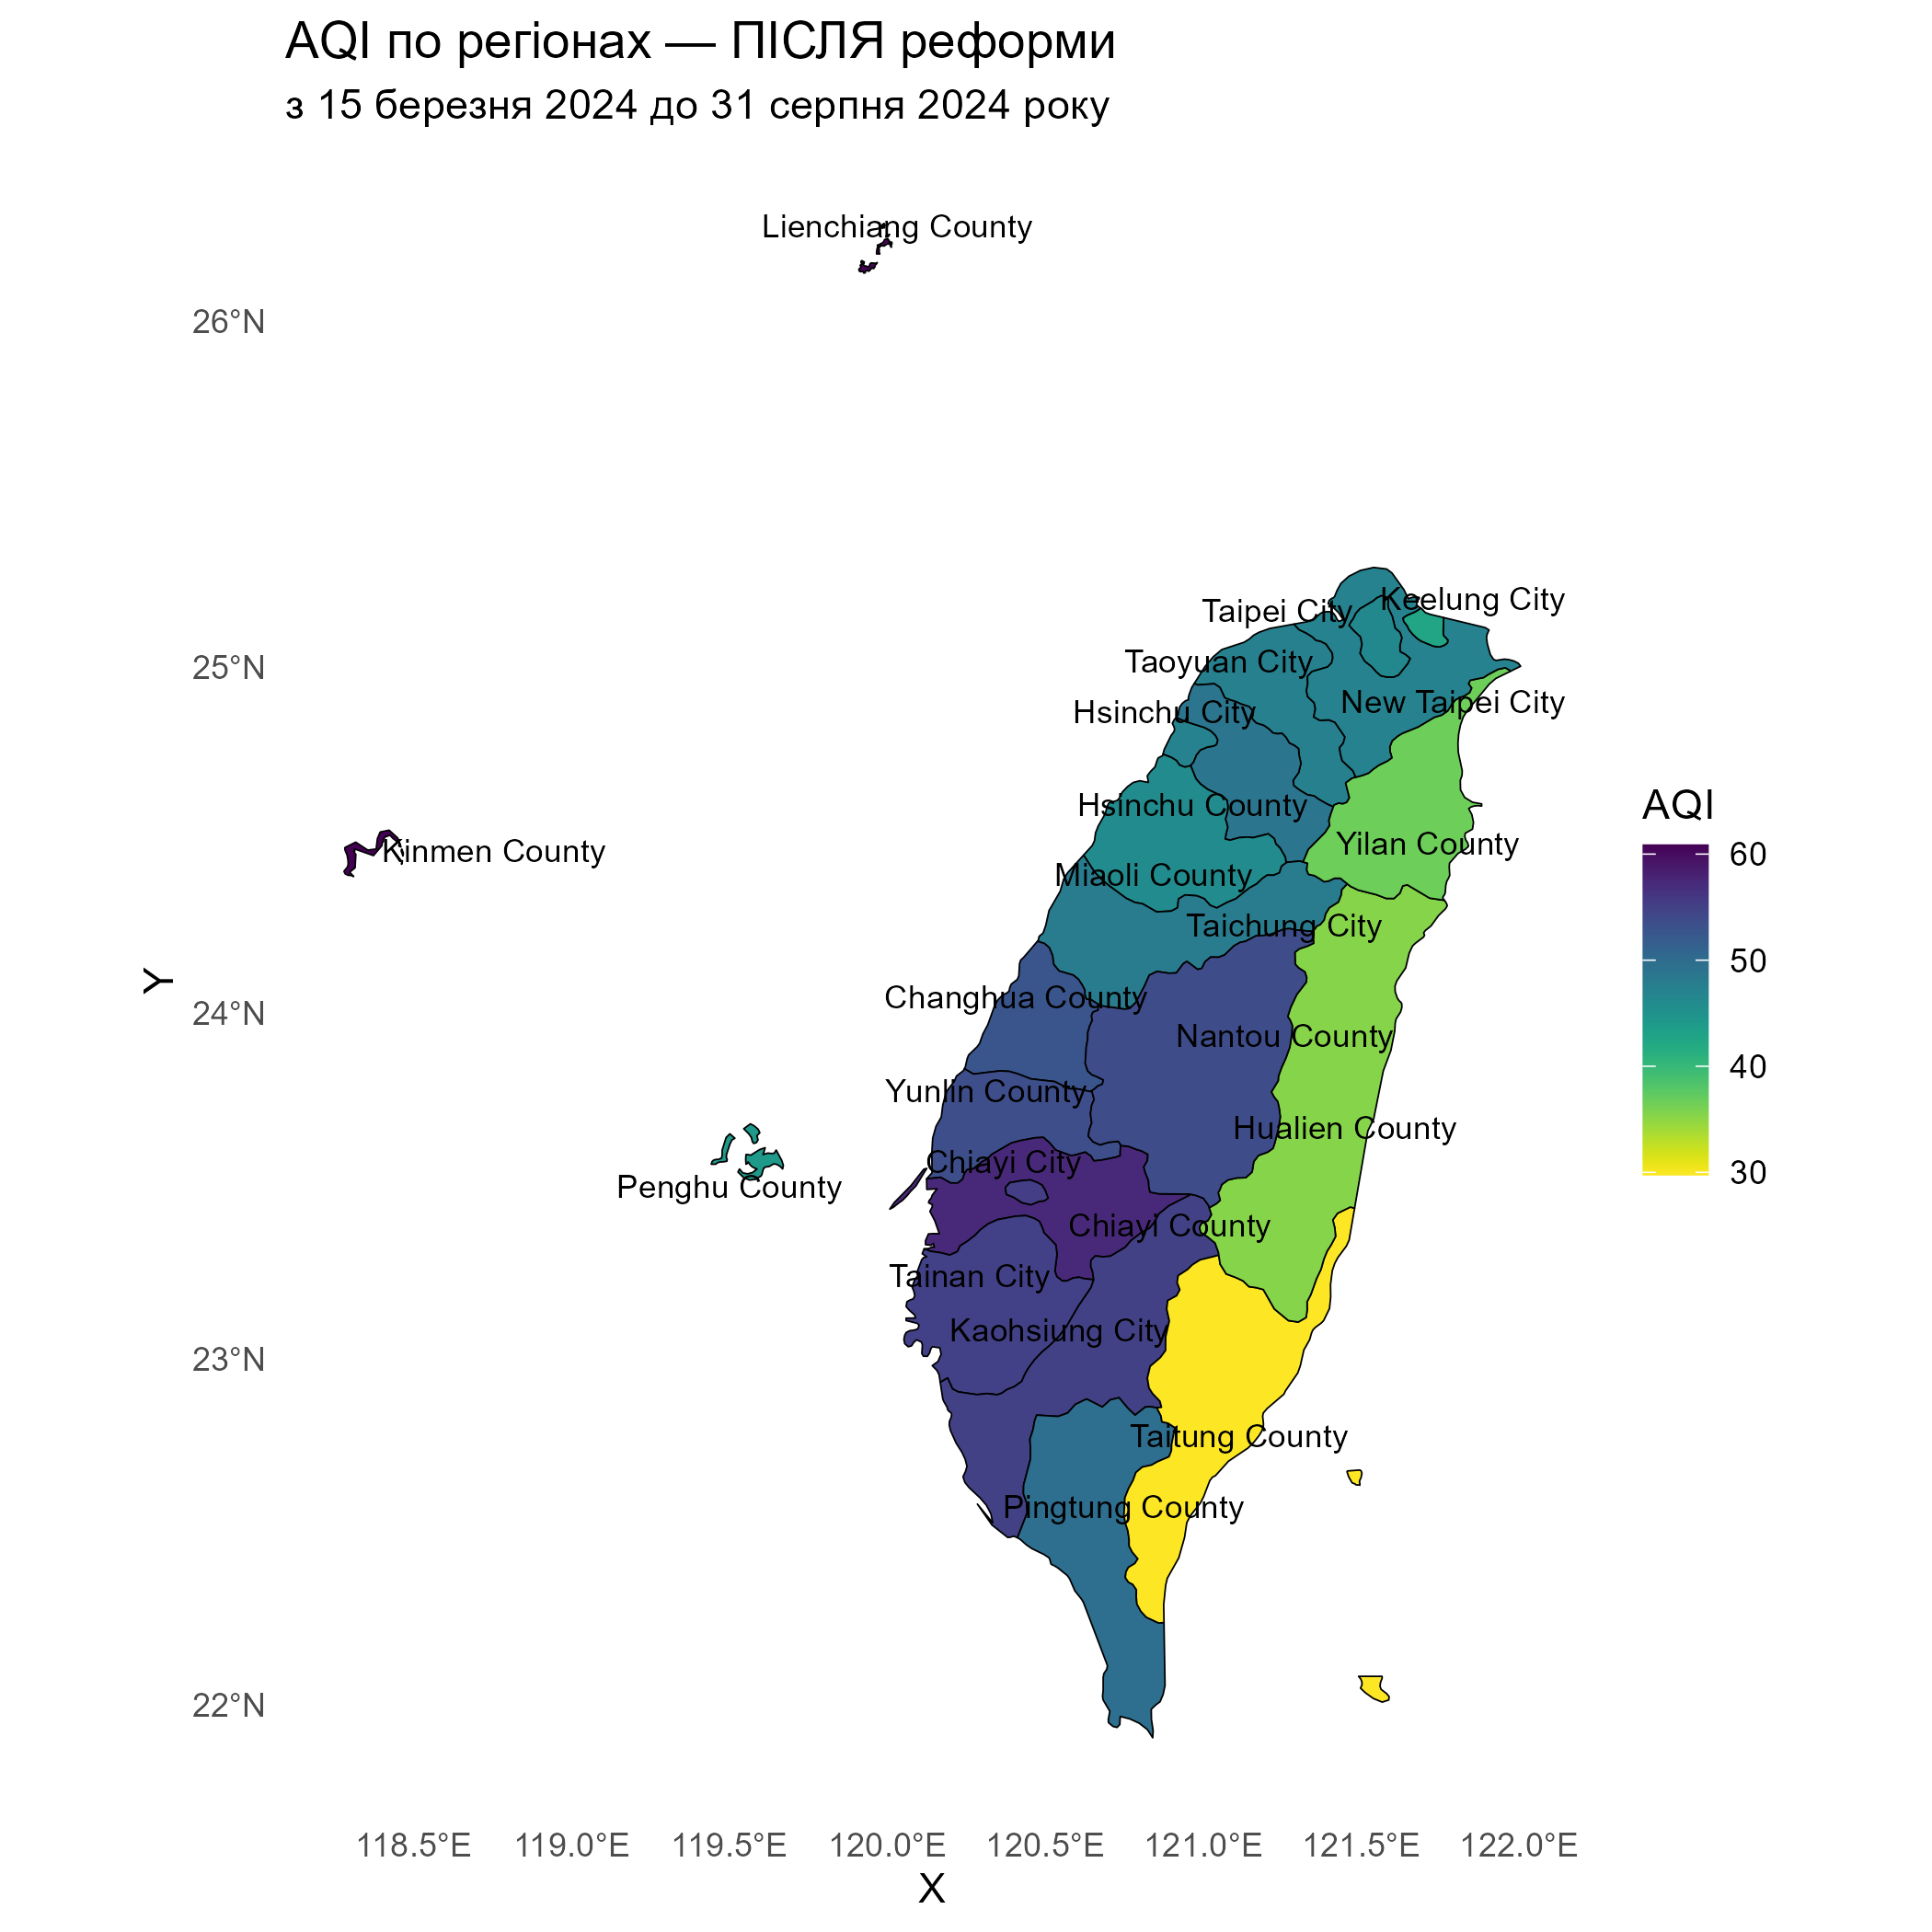
\includegraphics[height=2in]{plots/question5/map_after_reform.png}
    \end{tabular}
  \end{center}
\end{frame}

\begin{frame}
  \frametitle{Як змінився загальний рівень забруднення по регіонам після початку реформи?}

  \begin{center}
    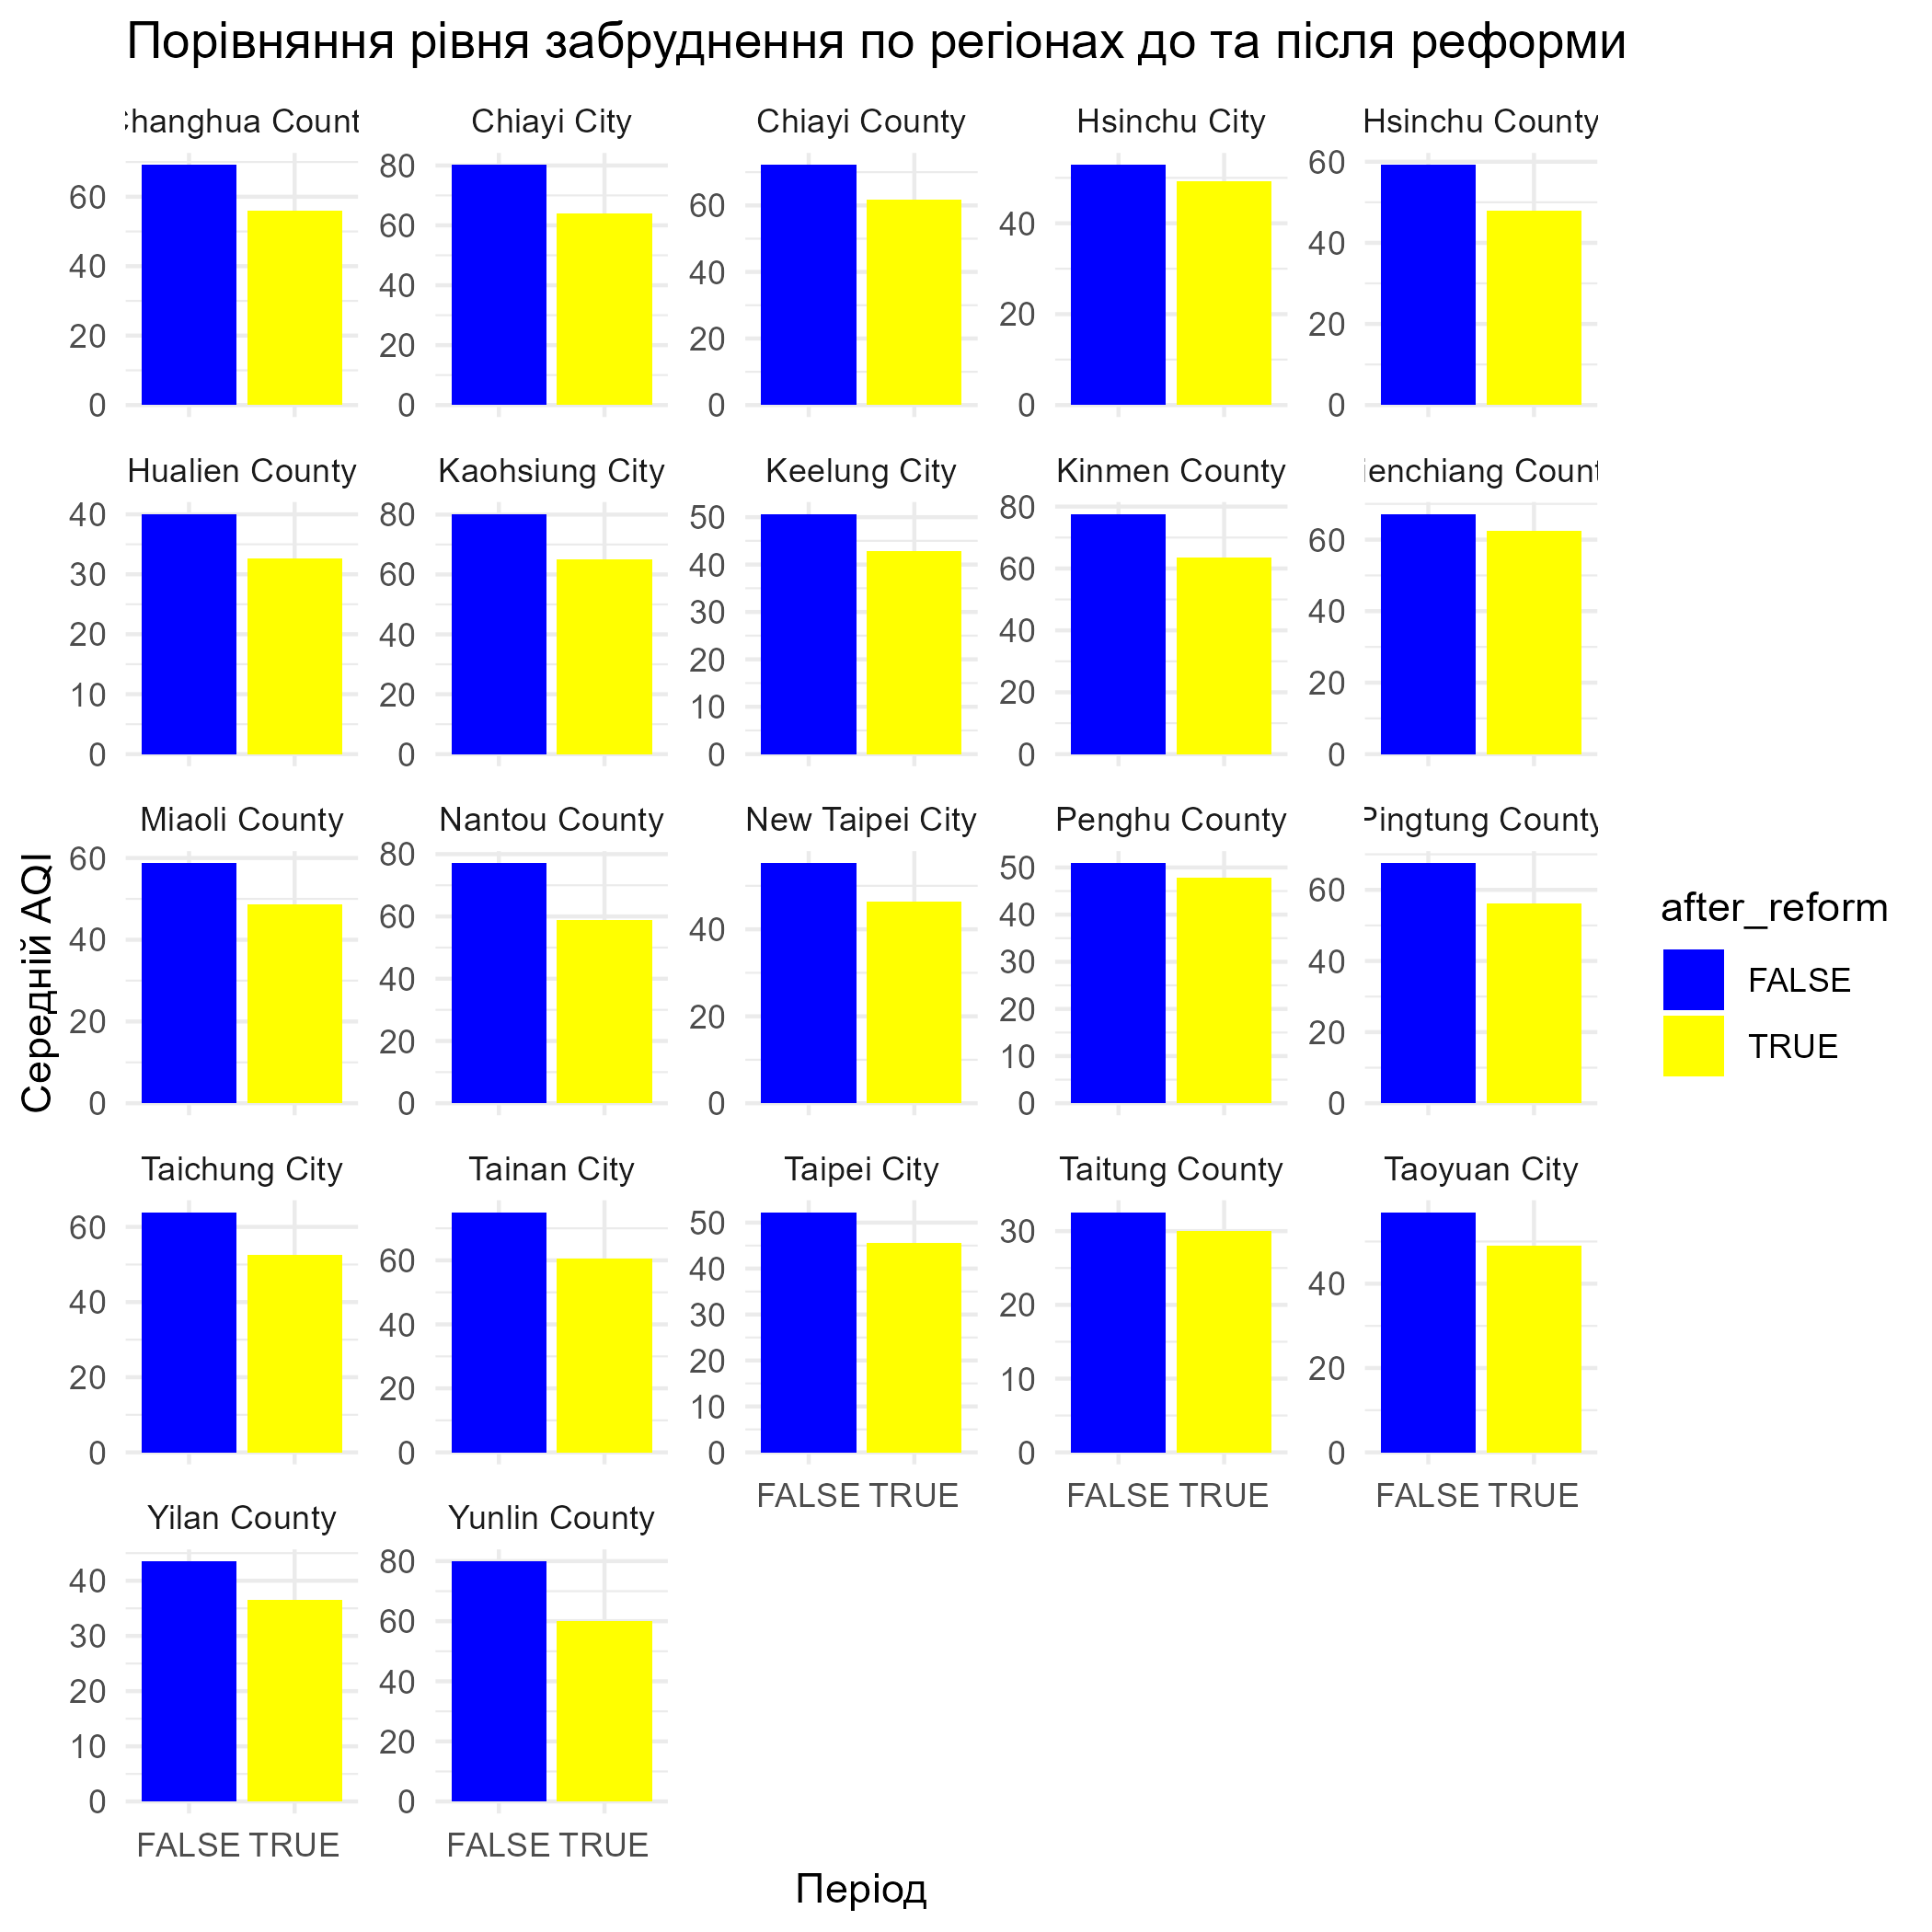
\includegraphics[height=2.8in]{plots/question5/region_comparison_aqi.png}
  \end{center}
\end{frame}

%% Question 6

\begin{frame}
  \frametitle{Чи існує залежність між початком реформ та показниками забруднення?}

  \textit{Був використаний tidy набір даних}

  \begin{center}
    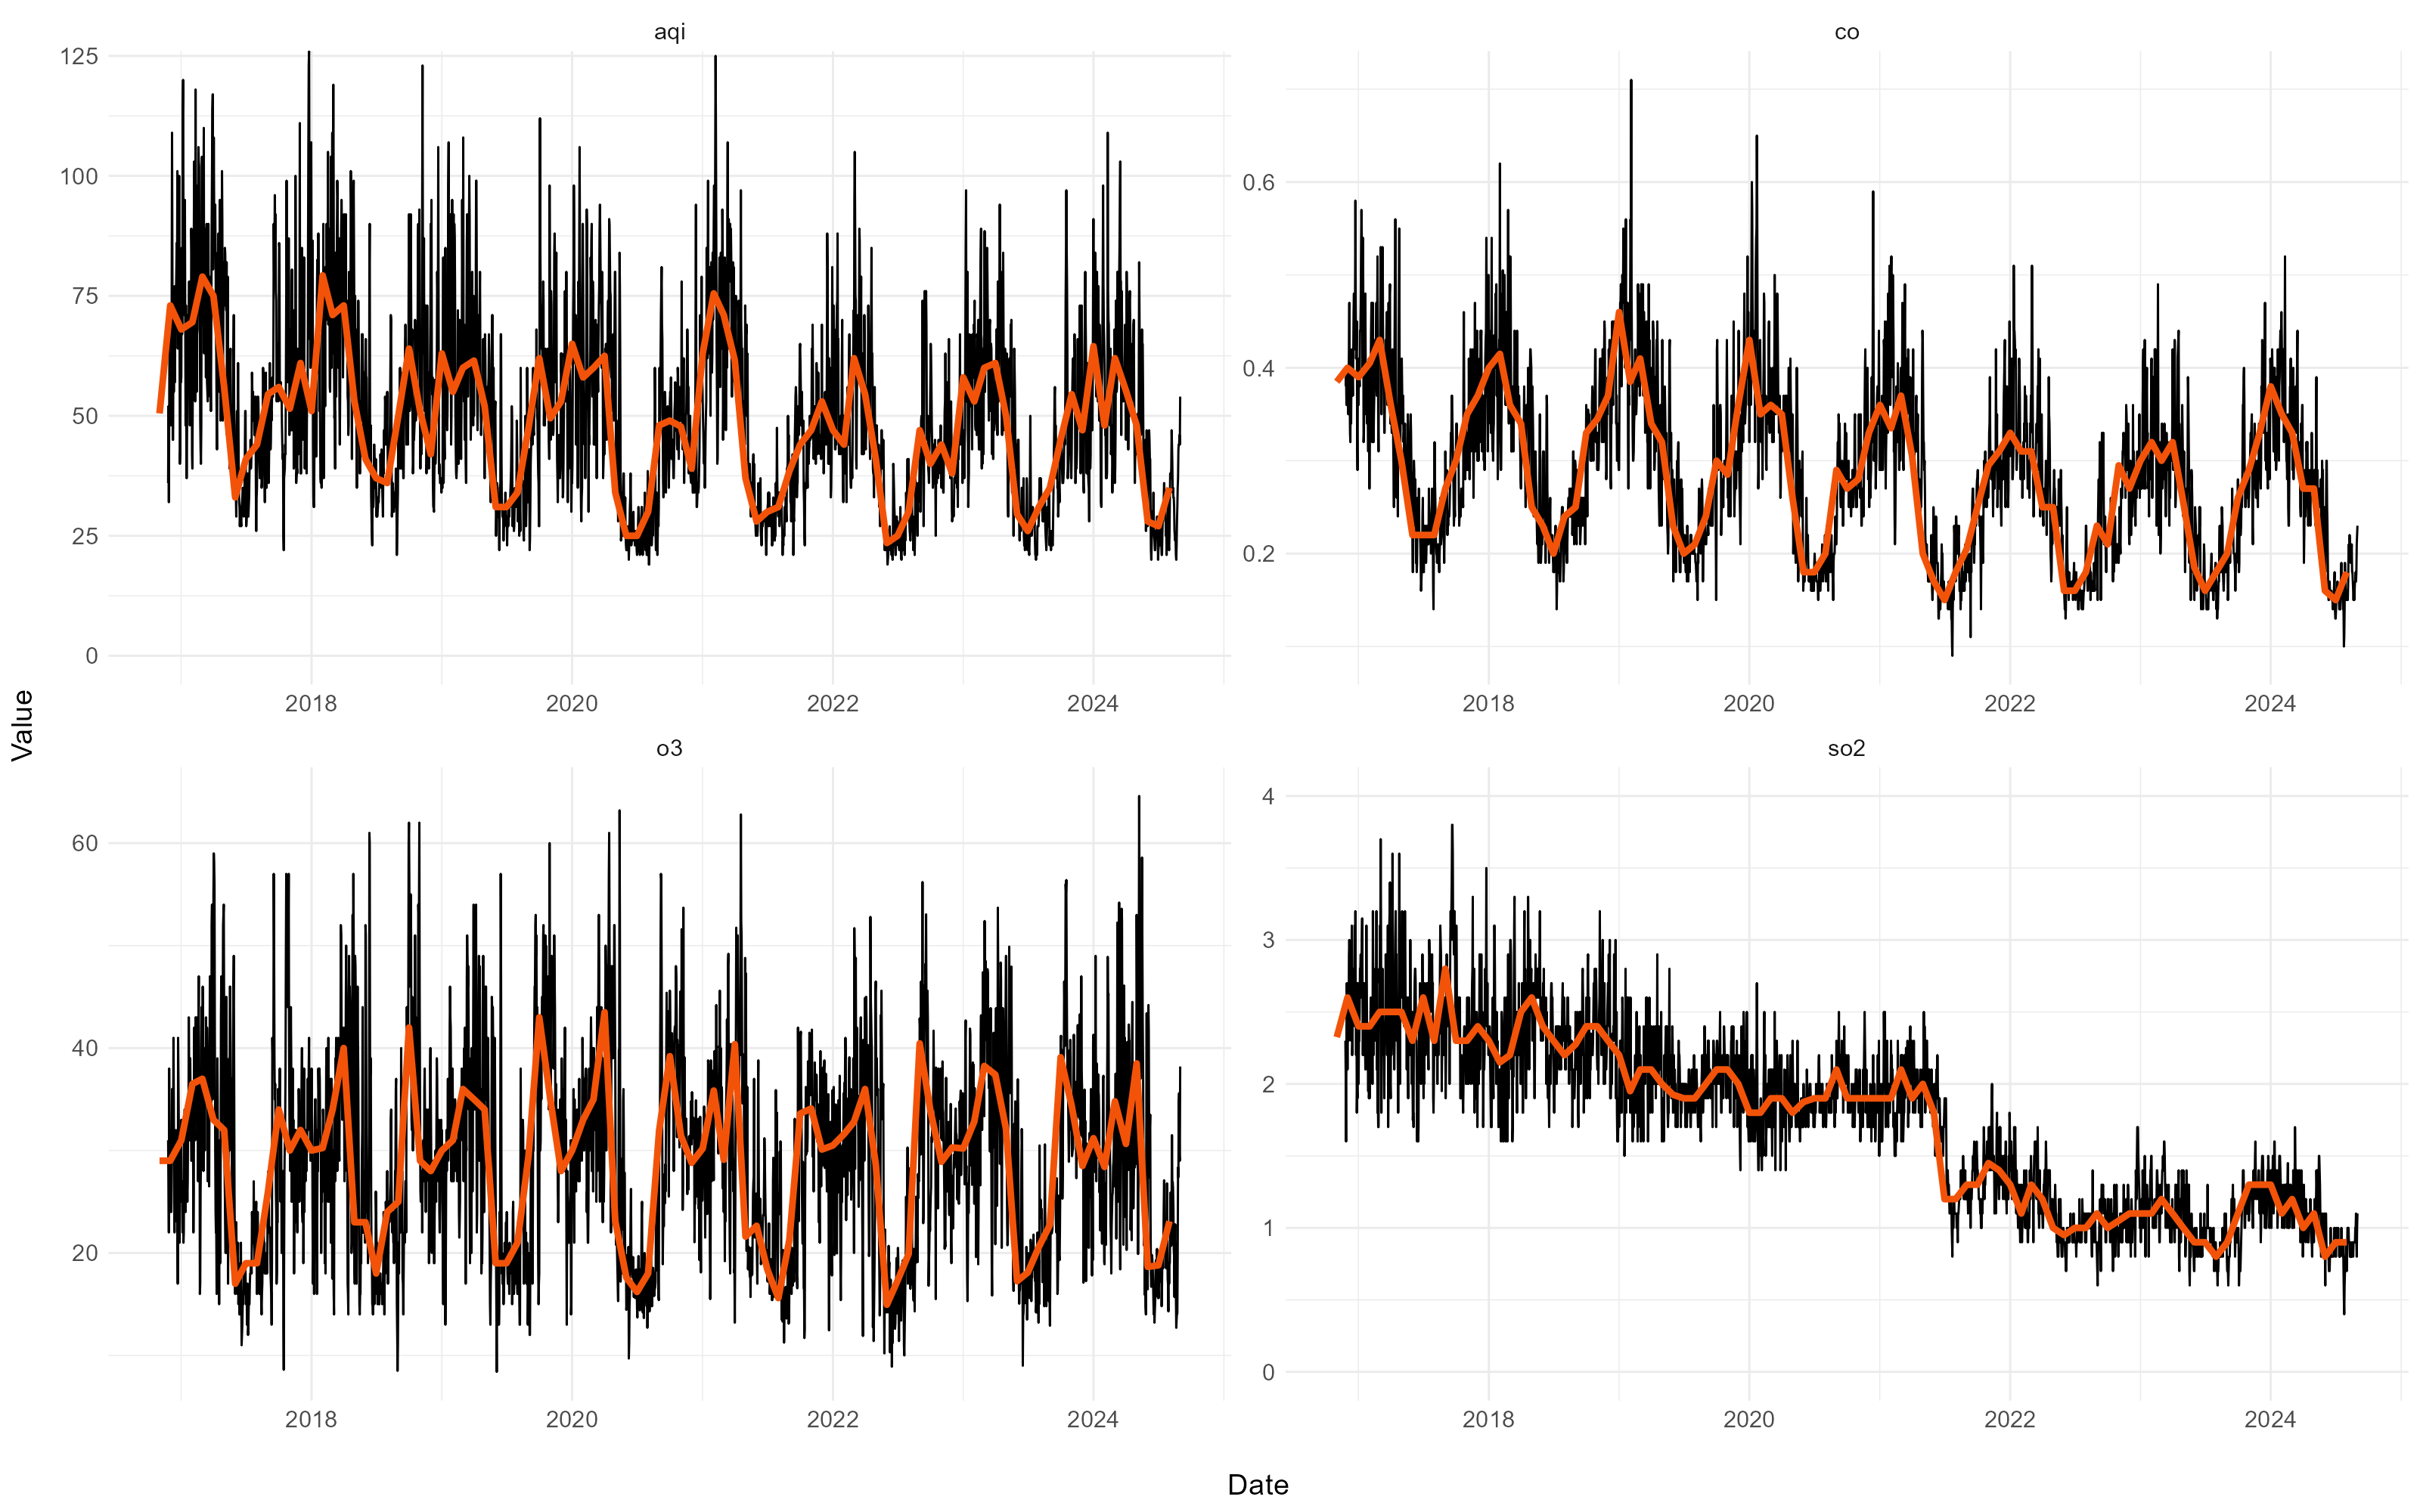
\includegraphics[height=2.5in]{plots/question6/line-p1.png}
  \end{center}
\end{frame}

\begin{frame}
  \frametitle{Чи існує залежність між початком реформ та показниками забруднення?}

  \begin{center}
    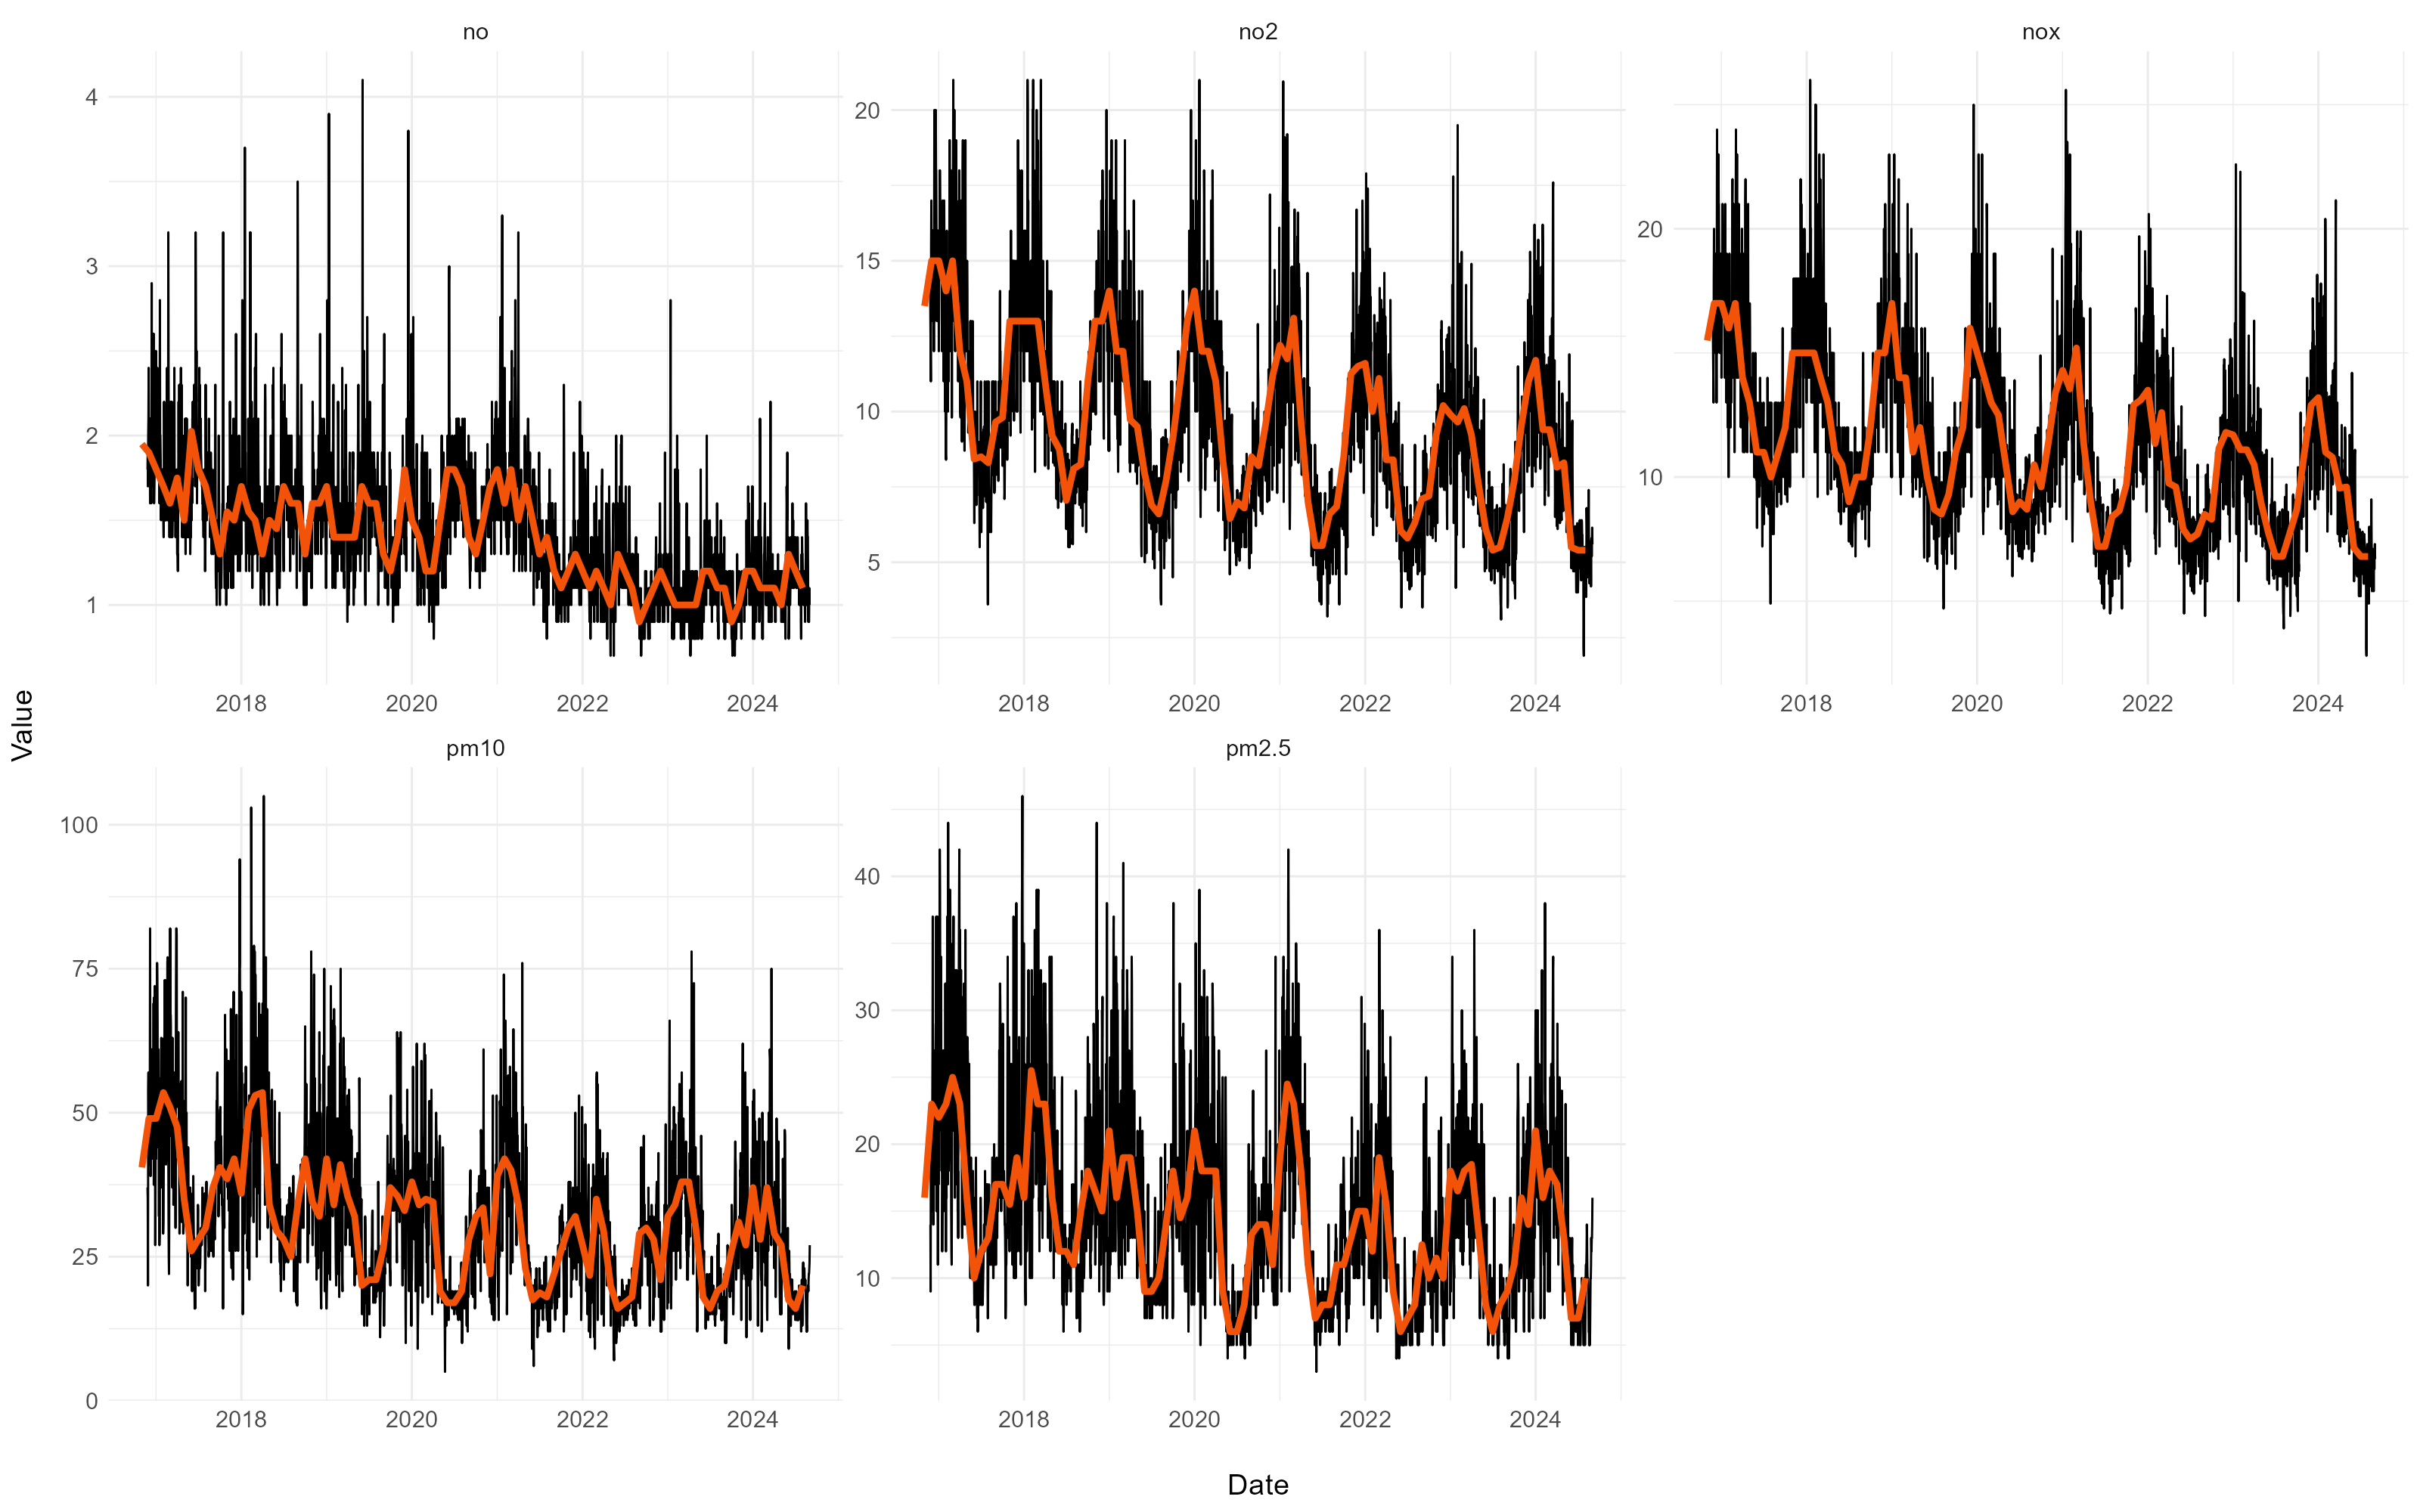
\includegraphics[height=2.8in]{plots/question6/line-p2.png}
  \end{center}
\end{frame}

%% Question 7

\begin{frame}
  \frametitle{Як змінюється якість повітря залежно від станції виміру у містах?}

  \textit{Був використаний trimmed набір даних}

  \begin{enumerate}
    \item Будемо розглядати зміни в показниках якості повітря в певній точці в часі (наприклад, 2023-06-28 11:00:00) в
    конкретному регіоні (наприклад, Tainan).
    \item Таким чином, будемо розглядати датасет згрупований за парою \textit{(date; county)}, так як тільки $sitename$ різний в групі.
  \end{enumerate}
\end{frame}

\begin{frame}
  \frametitle{Як змінюється якість повітря залежно від станції виміру у містах?}

  Порахуємо узагальнену статистику по кількості рядків в кожній групі:

  \begin{center}
    \begin{tabular}{lc}
      \textbf{Min.}    & 1     \\
      \textbf{1st Qu.} & 1     \\
      \textbf{Median}  & 3     \\
      \textbf{Mean}    & 3.864 \\
      \textbf{3rd Qu.} & 5     \\
      \textbf{Max.}    & 26    \\
    \end{tabular}
  \end{center}
\end{frame}

\begin{frame}
  \frametitle{Як змінюється якість повітря залежно від станції виміру у містах?}

  \begin{center}
    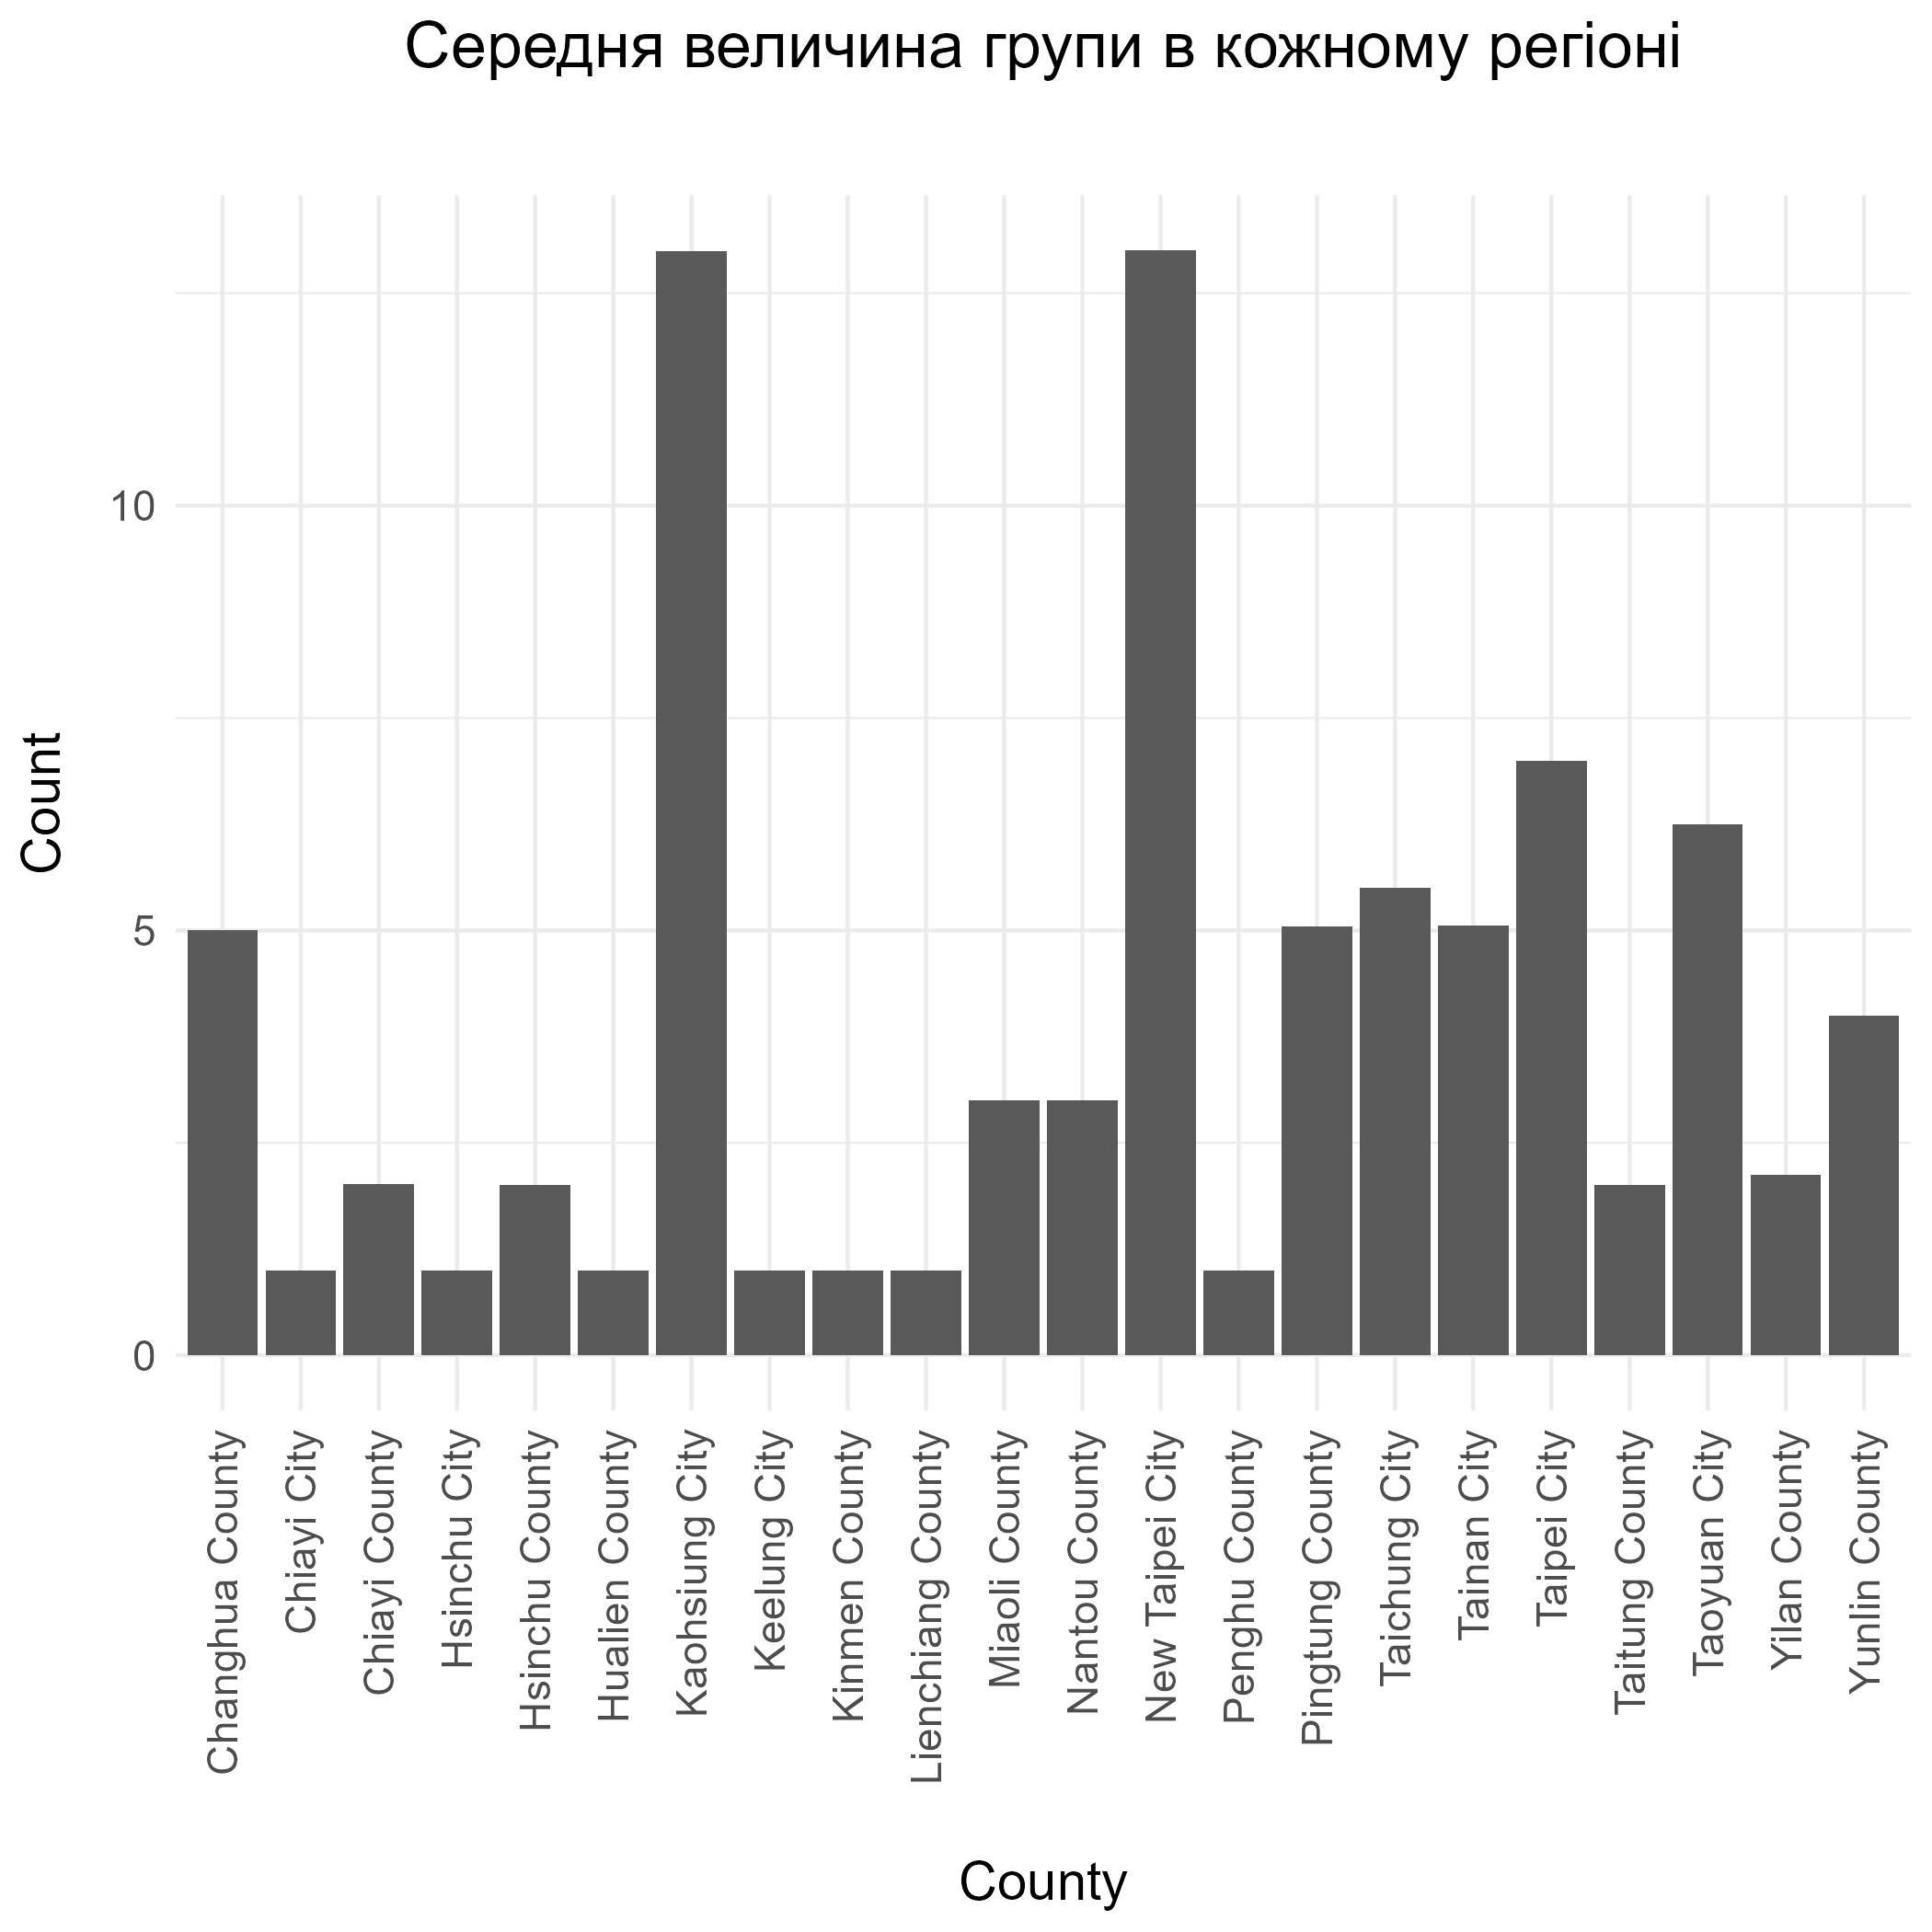
\includegraphics[height=2.8in]{plots/question7/bar-count.png}
  \end{center}
\end{frame}

\begin{frame}
  \frametitle{Як змінюється якість повітря залежно від станції виміру у містах?}

  Для аналізу змін в групі, будемо використовувати \textit{Median absolute difference}.

  \begin{center}
    \begin{tabular}{lcccccc}
      \hline
      \textbf{Variable} & \textbf{Min.} & \textbf{1st Qu.}  & \textbf{Median} & \textbf{Mean} & \textbf{3rd Qu.} & \textbf{Max.} \\
      \hline
      \textbf{aqi}      & 0             & 0                 & 2.965           & 4.597         & 6.672            & 109.712       \\
      \textbf{so2}      & 0             & 0                 & 0.2224          & 0.2989        & 0.4448           & 58.8592       \\
      \textbf{co}       & 0             & 0                 & 0.0222          & 0.0405        & 0.0593           & 4.0846        \\
      \textbf{o3}       & 0             & 0                 & 2.076           & 3.268         & 5.041            & 56.191        \\
      \textbf{pm10}     & 0             & 0                 & 2.965           & 4.265         & 5.930            & 254.266       \\
      \textbf{pm2.5}    & 0             & 0                 & 1.483           & 2.424         & 3.707            & 137.141       \\
      \textbf{no2}      & 0             & 0                 & 1.038           & 2.026         & 2.965            & 36.472        \\
      \textbf{nox}      & 0             & 0                 & 1.26            & 2.57          & 3.558            & 71.61         \\
      \textbf{no}       & 0             & 0                 & 0.2965          & 0.6151        & 0.593            & 62.2692       \\
    \end{tabular}
  \end{center}
\end{frame}

\begin{frame}
  \frametitle{Як змінюється якість повітря залежно від станції виміру у містах?}

  \begin{center}
    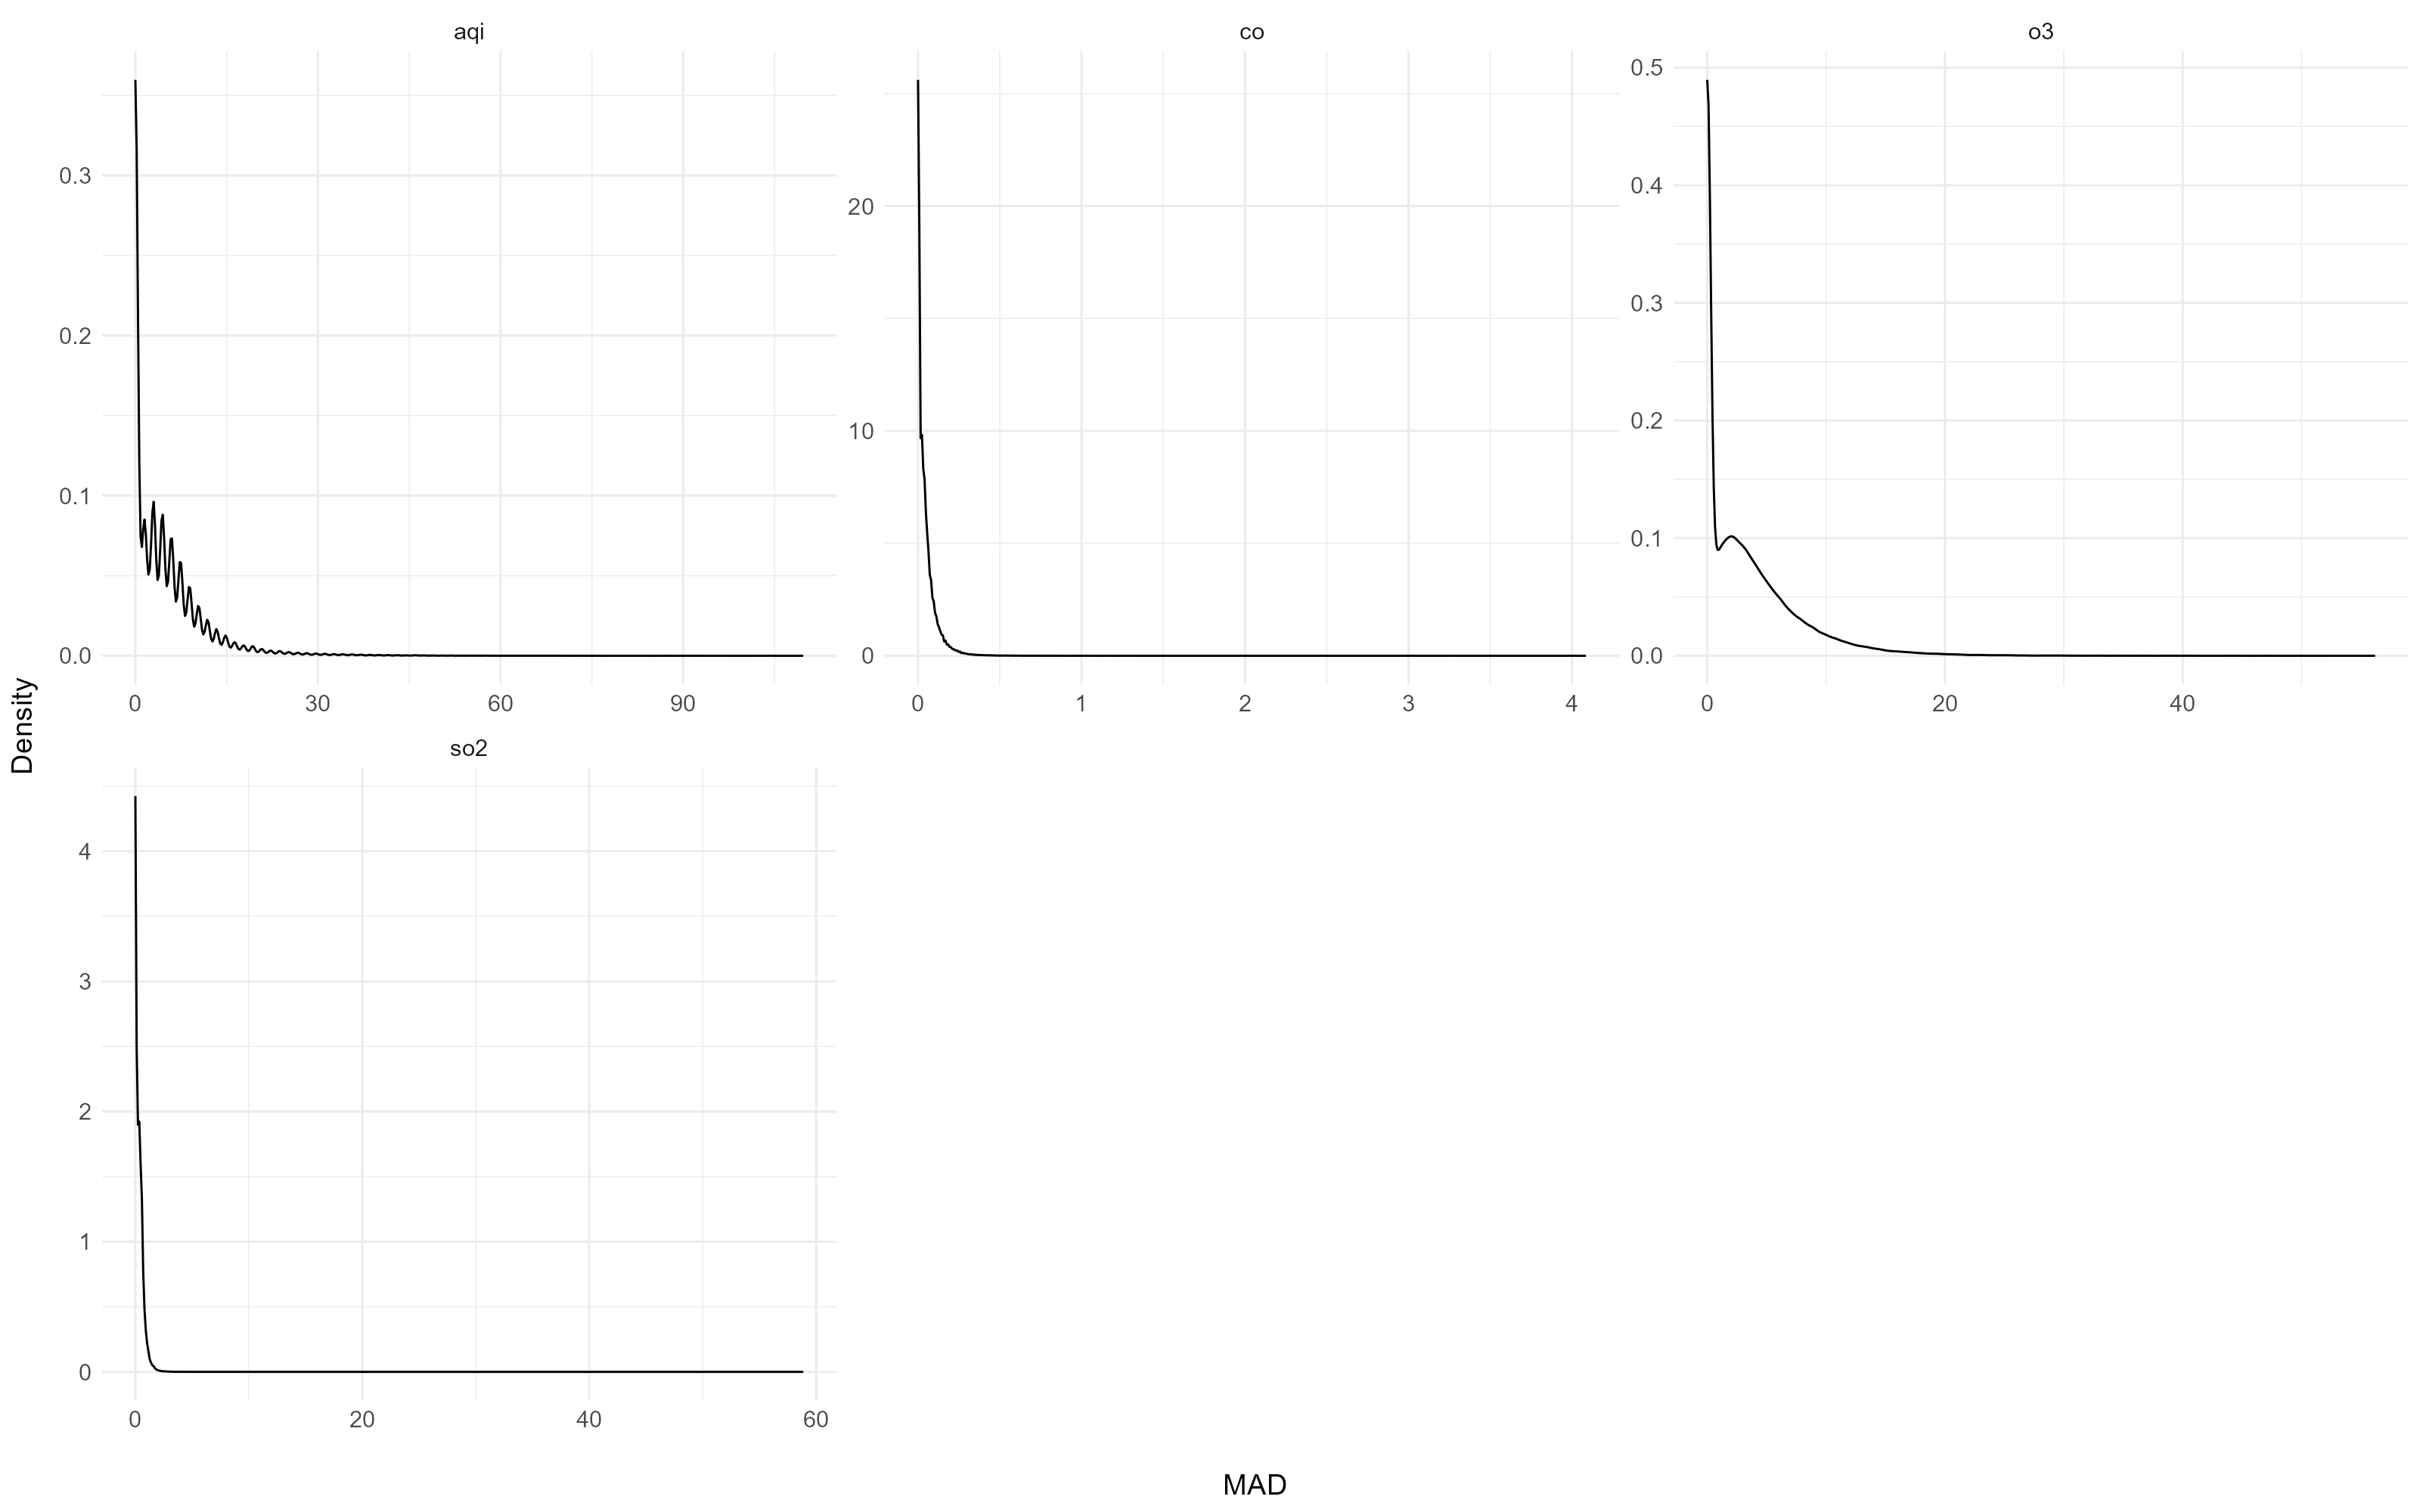
\includegraphics[height=2.8in]{plots/question7/density-p1.png}
  \end{center}
\end{frame}

\begin{frame}
  \frametitle{Як змінюється якість повітря залежно від станції виміру у містах?}

  \begin{center}
    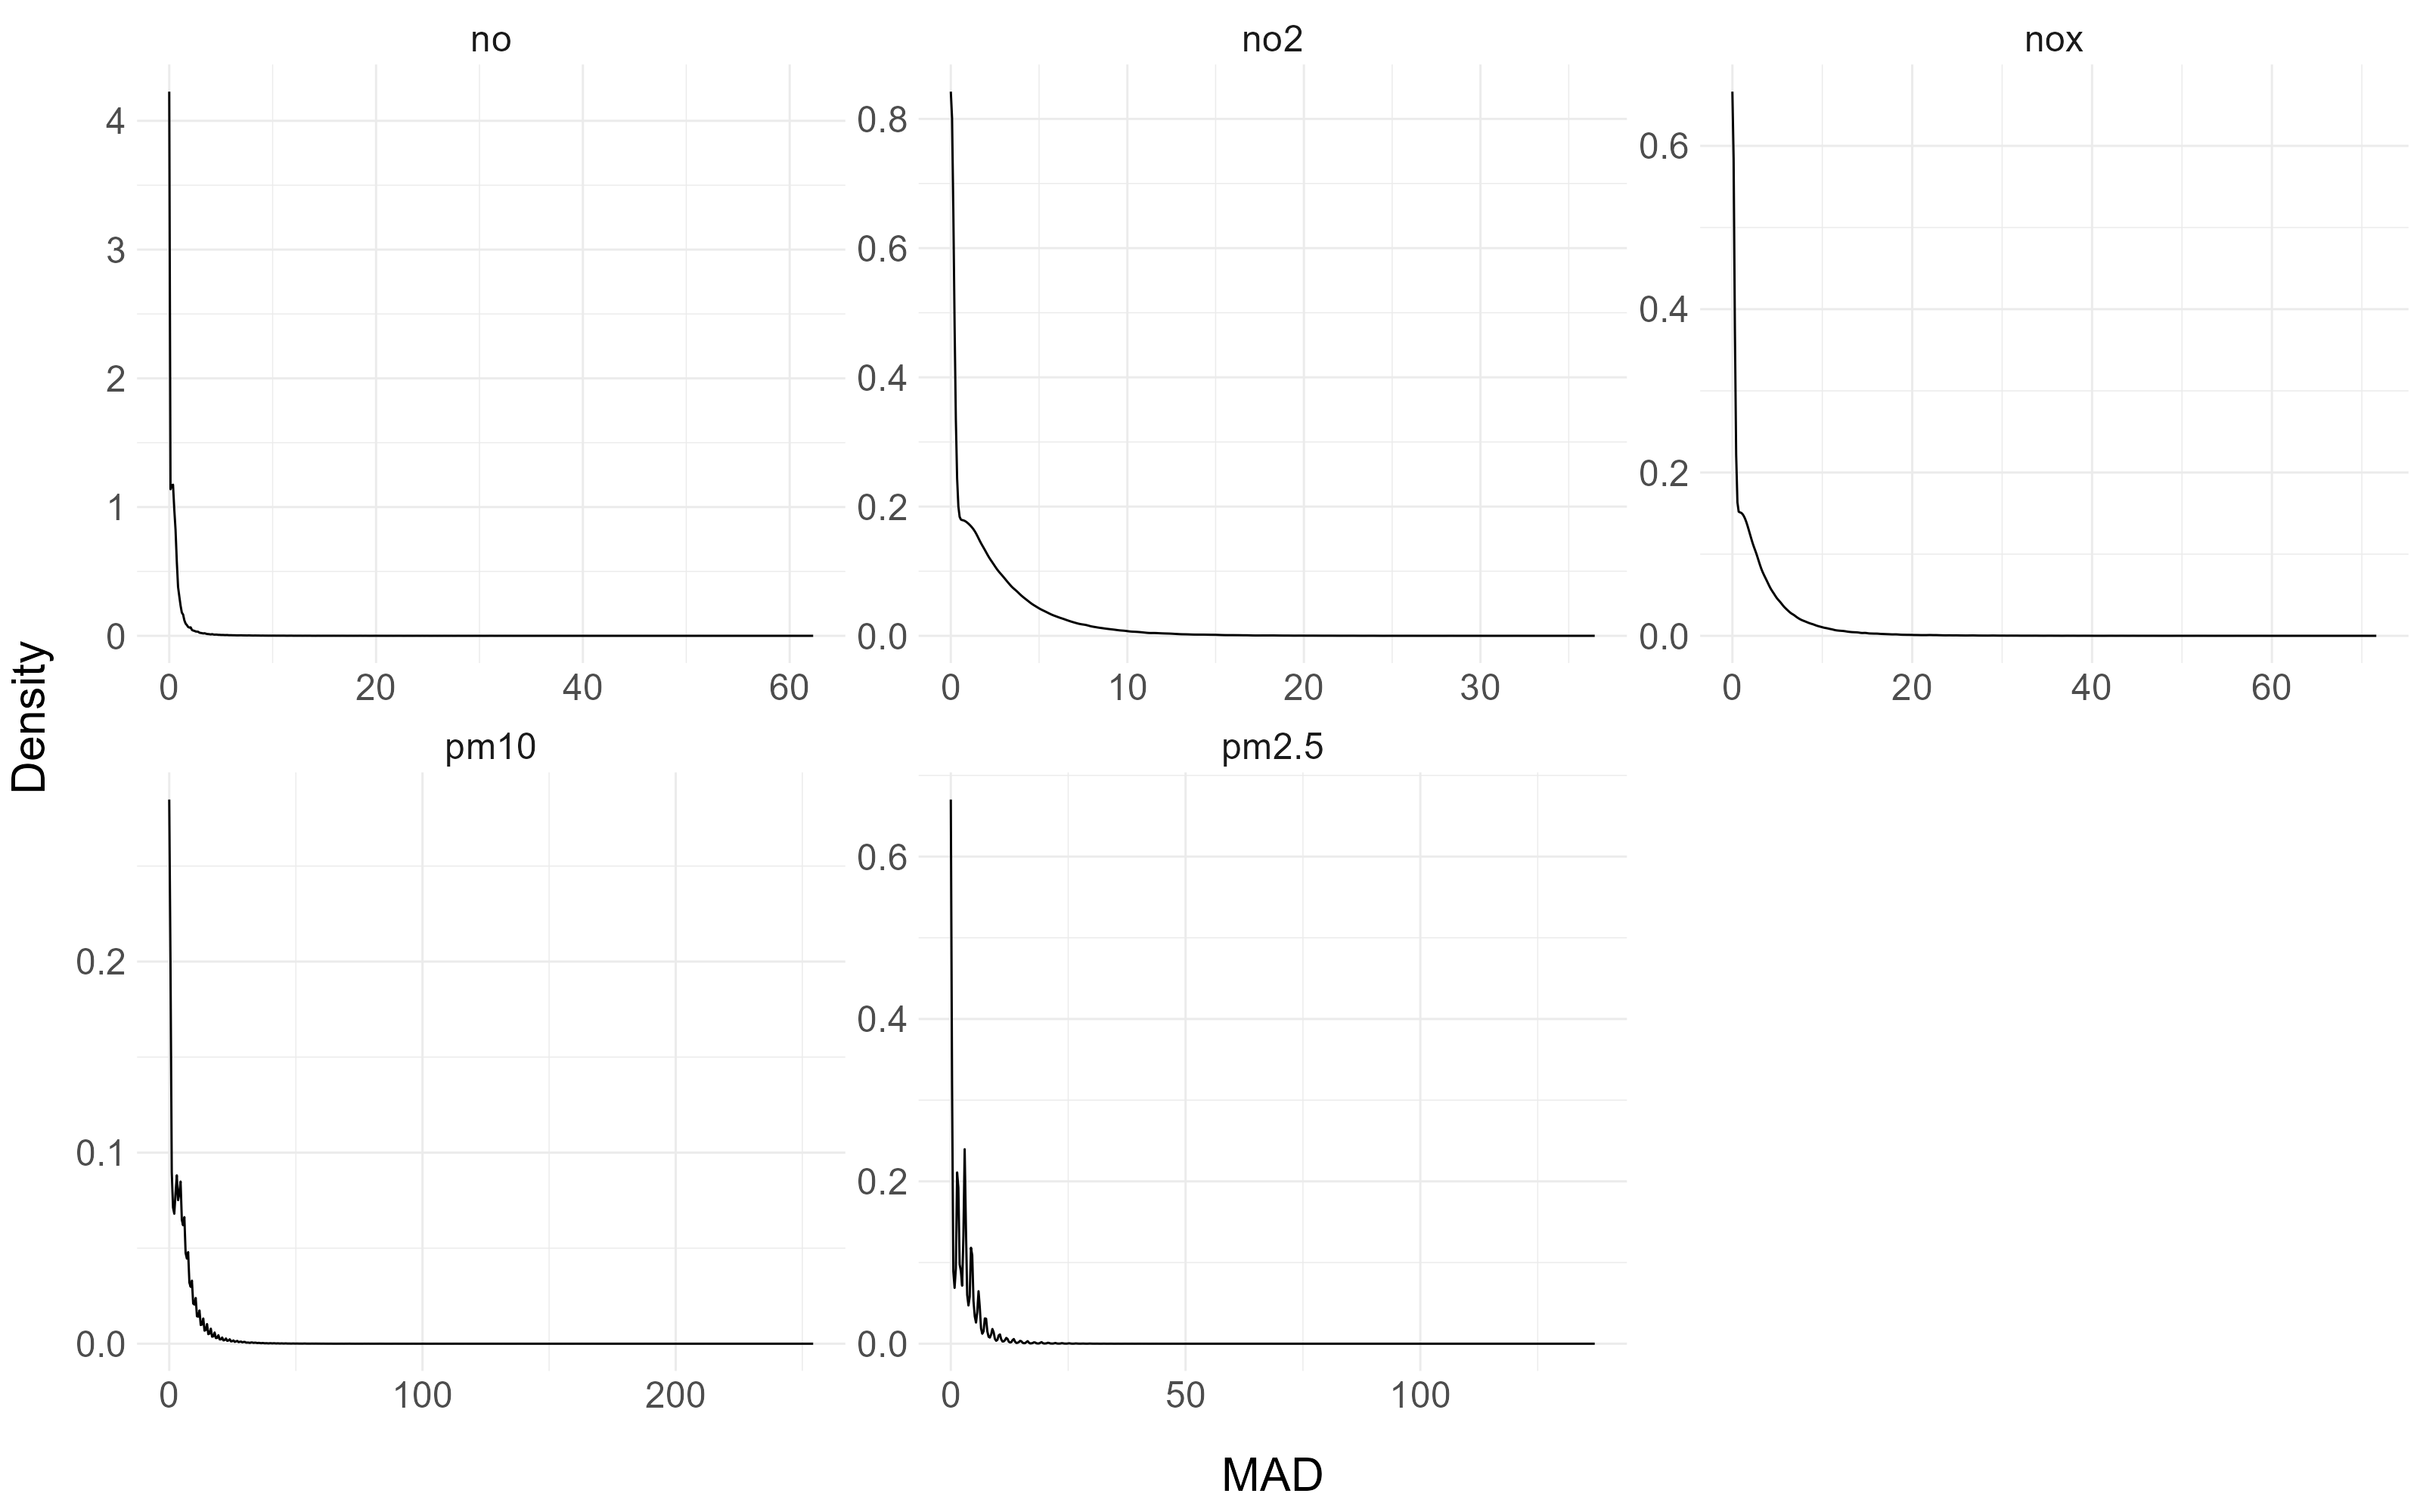
\includegraphics[height=2.8in]{plots/question7/density-p2.png}
  \end{center}
\end{frame}

\begin{frame}
  \frametitle{Як змінюється якість повітря залежно від станції виміру у містах?}

  \begin{center}
    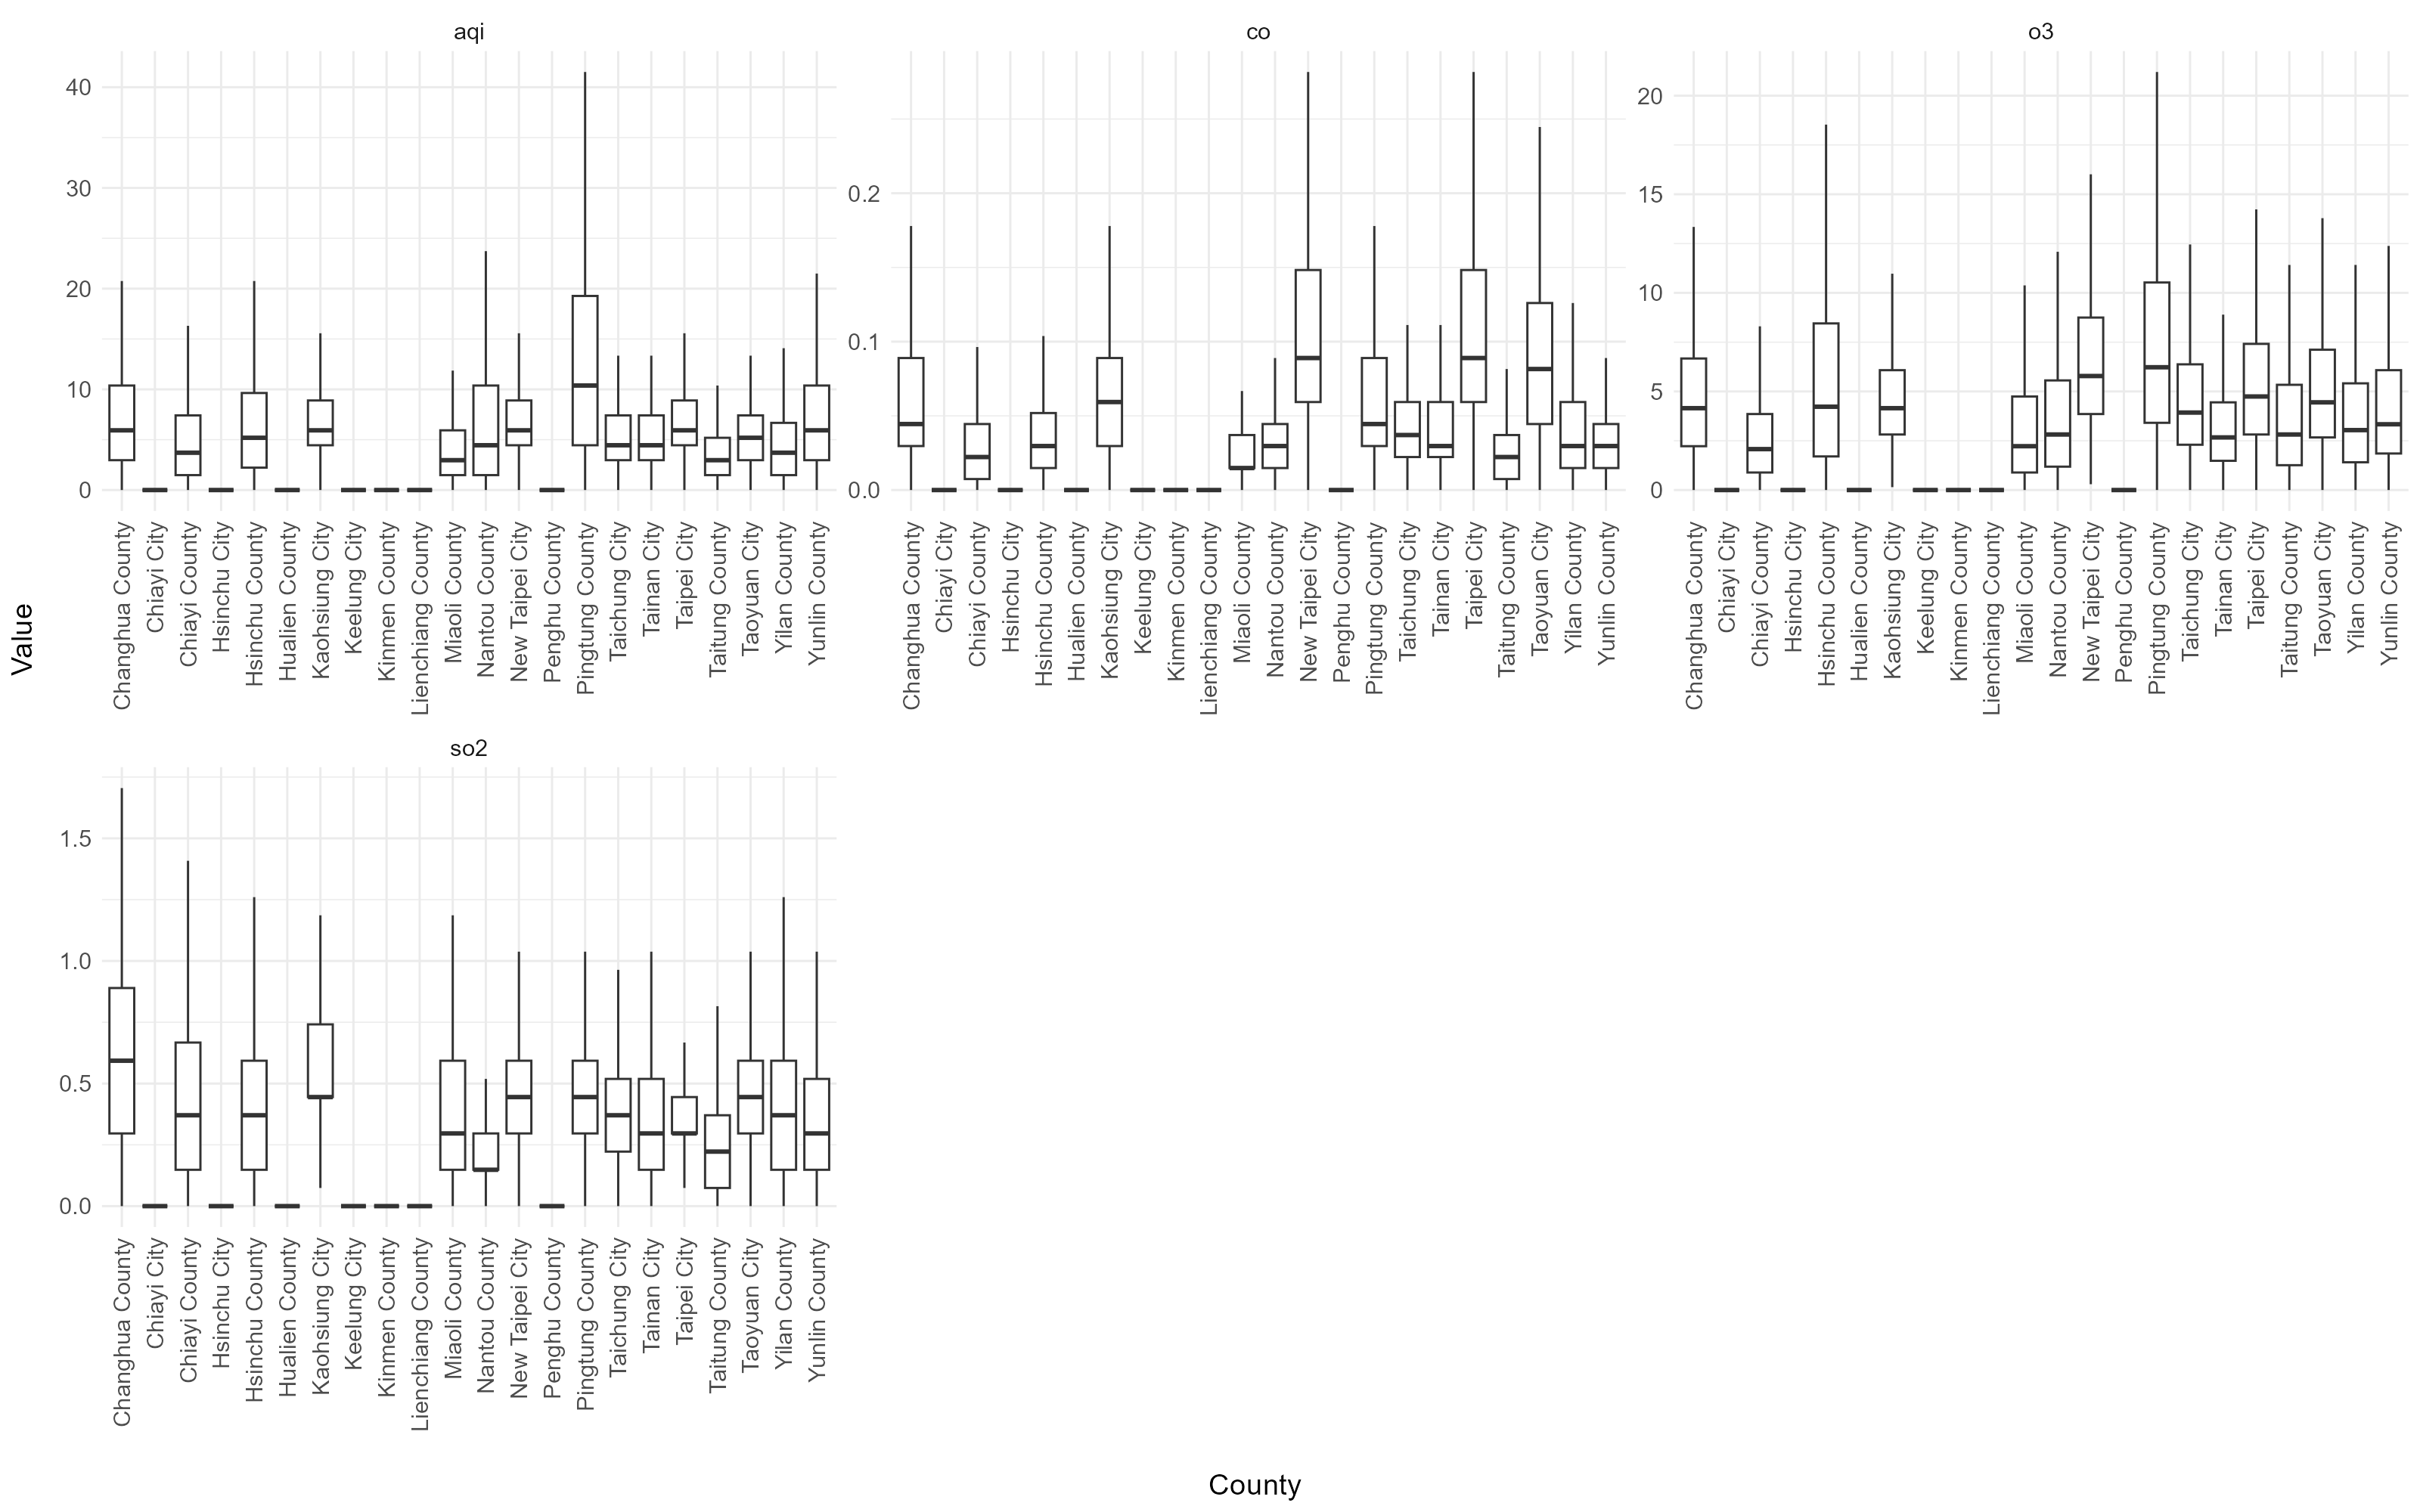
\includegraphics[height=2.8in]{plots/question7/box-county-p1.png}
  \end{center}
\end{frame}

\begin{frame}
  \frametitle{Як змінюється якість повітря залежно від станції виміру у містах?}

  \begin{center}
    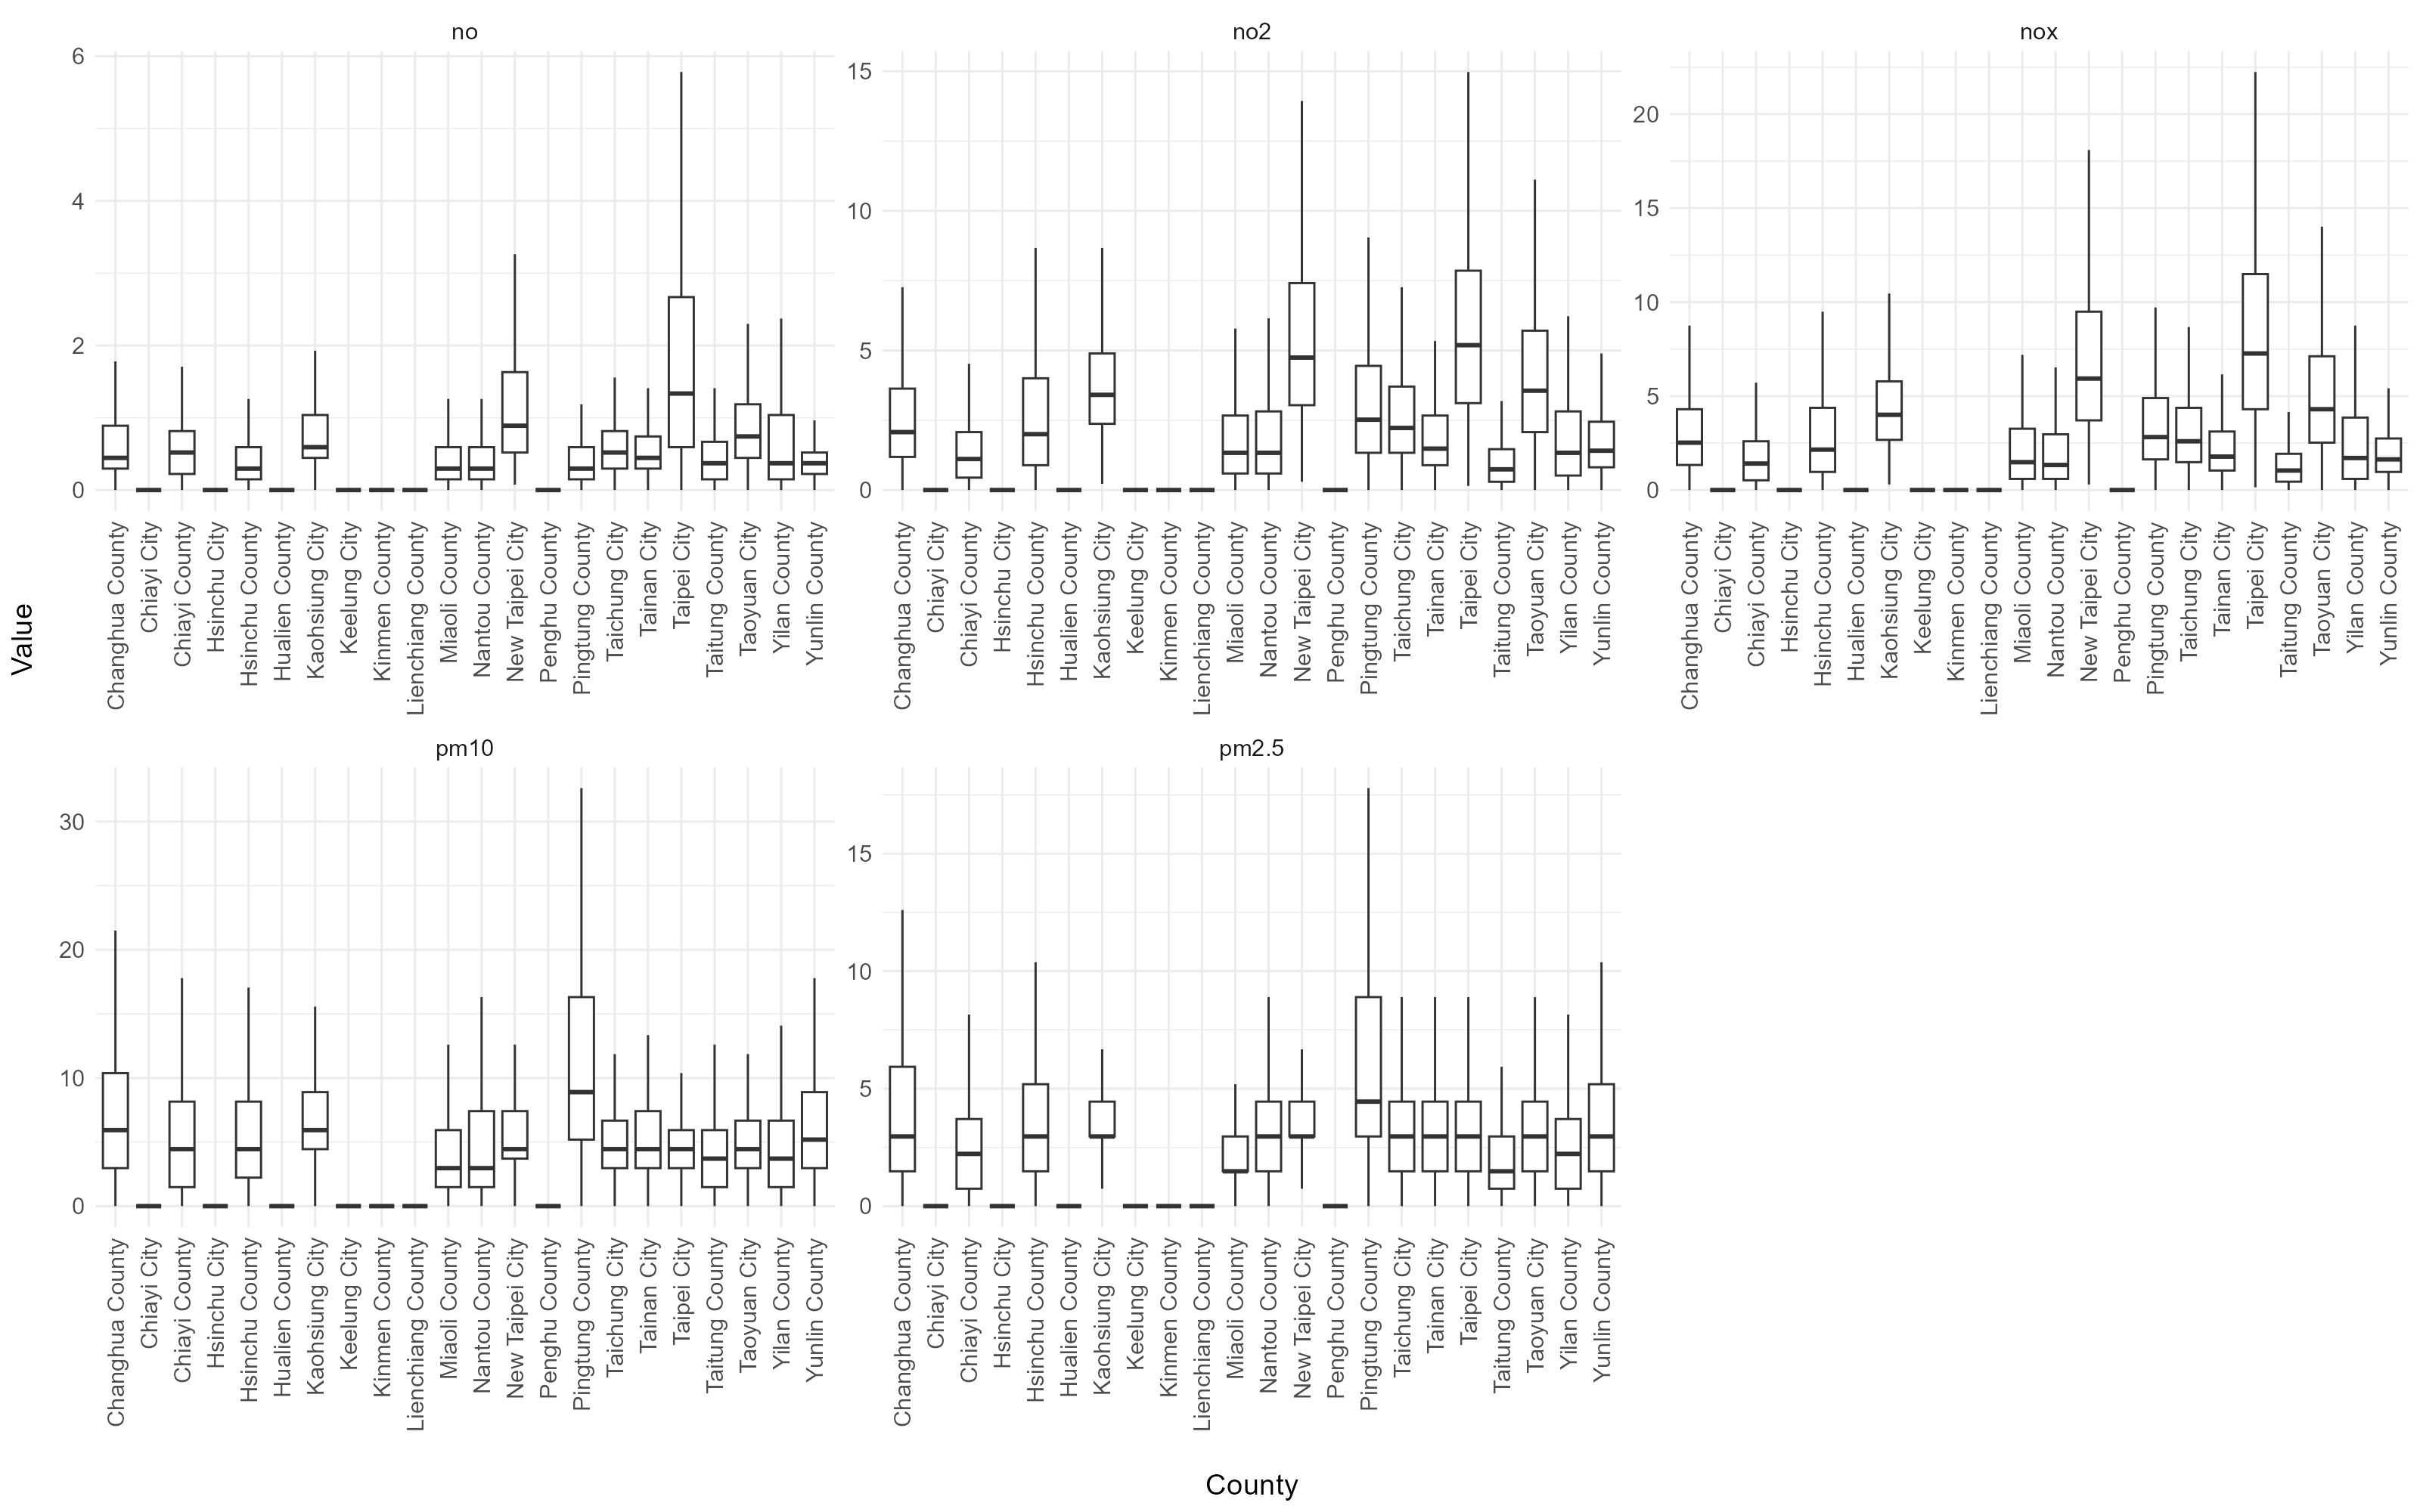
\includegraphics[height=2.8in]{plots/question7/box-county-p2.png}
  \end{center}
\end{frame}

\end{document}